% **************************************************************************************************************
% A Classic Thesis Style
% An Homage to The Elements of Typographic Style
%
% Copyright (C) 2015 André Miede http://www.miede.de
%
% If you like the style then I would appreciate a postcard. My address 
% can be found in the file ClassicThesis.pdf. A collection of the 
% postcards I received so far is available online at 
% http://postcards.miede.de
%
% License:
% This program is free software; you can redistribute it and/or modify
% it under the terms of the GNU General Public License as published by
% the Free Software Foundation; either version 2 of the License, or
% (at your option) any later version.
%
% This program is distributed in the hope that it will be useful,
% but WITHOUT ANY WARRANTY; without even the implied warranty of
% MERCHANTABILITY or FITNESS FOR A PARTICULAR PURPOSE.  See the
% GNU General Public License for more details.
%
% You should have received a copy of the GNU General Public License
% along with this program; see the file COPYING.  If not, write to
% the Free Software Foundation, Inc., 59 Temple Place - Suite 330,
% Boston, MA 02111-1307, USA.   
%
% **************************************************************************************************************
\RequirePackage{fix-cm} % fix some latex issues see: http://texdoc.net/texmf-dist/doc/latex/base/fixltx2e.pdf
\documentclass[ oneside,openany,titlepage,numbers=noenddot,headinclude,%1headlines,% letterpaper a4paper
                footinclude=true,cleardoublepage=empty,abstractoff, % <--- obsolete, remove (todo)
                BCOR=5mm,paper=a4,fontsize=11pt,%11pt,a4paper,%
                spanish,american%
                ]{scrreprt}

%********************************************************************
% Note: Make all your adjustments in here
%*******************************************************
% ****************************************************************************************************
% classicthesis-config.tex 
% formerly known as loadpackages.sty, classicthesis-ldpkg.sty, and classicthesis-preamble.sty 
% Use it at the beginning of your ClassicThesis.tex, or as a LaTeX Preamble 
% in your ClassicThesis.{tex,lyx} with % ****************************************************************************************************
% classicthesis-config.tex 
% formerly known as loadpackages.sty, classicthesis-ldpkg.sty, and classicthesis-preamble.sty 
% Use it at the beginning of your ClassicThesis.tex, or as a LaTeX Preamble 
% in your ClassicThesis.{tex,lyx} with % ****************************************************************************************************
% classicthesis-config.tex 
% formerly known as loadpackages.sty, classicthesis-ldpkg.sty, and classicthesis-preamble.sty 
% Use it at the beginning of your ClassicThesis.tex, or as a LaTeX Preamble 
% in your ClassicThesis.{tex,lyx} with \input{classicthesis-config}
% ****************************************************************************************************  
% If you like the classicthesis, then I would appreciate a postcard. 
% My address can be found in the file ClassicThesis.pdf. A collection 
% of the postcards I received so far is available online at 
% http://postcards.miede.de
% ****************************************************************************************************


% ****************************************************************************************************
% 0. Set the encoding of your files. UTF-8 is the only sensible encoding nowadays. If you can't read
% äöüßáéçèê∂åëæƒÏ€ then change the encoding setting in your editor, not the line below. If your editor
% does not support utf8 use another editor!
% ****************************************************************************************************
\PassOptionsToPackage{utf8}{inputenc}
	\usepackage{inputenc}

% ****************************************************************************************************
% 1. Configure classicthesis for your needs here, e.g., remove "drafting" below 
% in order to deactivate the time-stamp on the pages
% ****************************************************************************************************
\PassOptionsToPackage{listings,eulerchapternumbers,%eulermath,%drafting,%
                      pdfspacing,floatperchapter,%linedheaders,%
                      beramono,
                      subfig,parts,dottedtoc}{classicthesis}                                        
% ********************************************************************
% Available options for classicthesis.sty 
% (see ClassicThesis.pdf for more information):
% drafting
% parts nochapters linedheaders
% eulerchapternumbers beramono eulermath pdfspacing minionprospacing
% tocaligned dottedtoc manychapters
% listings floatperchapter subfig
% ********************************************************************


% ****************************************************************************************************
% 2. Personal data and user ad-hoc commands
% ****************************************************************************************************
\newcommand{\myTitle}{Problema isoperimétrico en el espacio euclídeo. Representación de información imprecisa en base de datos NoSQL\xspace}
\newcommand{\mySubtitle}{ \xspace}
%\newcommand{\mySubtitle}{Resolución problema isoperimétrico y propuesta MongoDB\xspace}
\newcommand{\myWork}{Trabajo Fin de Grado}
\newcommand{\myDegree}{Doble Grado en Ingeniería Informática y Matemáticas\xspace}
\newcommand{\myName}{Sergio Padilla López\xspace}
\newcommand{\myProf}{César Rosales Lombardo\xspace}
\newcommand{\myOtherProf}{Juan Miguel Medina Rodríguez\xspace}
%\newcommand{\mySupervisor}{Put name here\xspace}
\newcommand{\myFaculty}{Facultad de Ciencias\xspace}
\newcommand{\myOtherFaculty}{Escuela Técnica Superior de Ingenierías Informática y de Telecomunicación\xspace}
\newcommand{\myOtherFacultyA}{Escuela Técnica Superior de Ingenierías\xspace}
\newcommand{\myOtherFacultyB}{Informática y de Telecomunicación\xspace}
%\newcommand{\myDepartment}{Put data here\xspace}
\newcommand{\myUni}{Universidad de Granada\xspace}
\newcommand{\myLocation}{Granada\xspace}
\newcommand{\myTime}{Junio de 2018\xspace}
%\newcommand{\myVersion}{version 4.2\xspace}

% ********************************************************************
% Setup, finetuning, and useful commands
% ********************************************************************
\newcounter{dummy} % necessary for correct hyperlinks (to index, bib, etc.)
\newlength{\abcd} % for ab..z string length calculation
\providecommand{\mLyX}{L\kern-.1667em\lower.25em\hbox{Y}\kern-.125emX\@}
\newcommand{\ie}{i.\,e.}
\newcommand{\Ie}{I.\,e.}
\newcommand{\eg}{e.\,g.}
\newcommand{\Eg}{E.\,g.} 
% ****************************************************************************************************


% ****************************************************************************************************
% 3. Loading some handy packages
% ****************************************************************************************************
% ******************************************************************** 
% Packages with options that might require adjustments
% ******************************************************************** 
%\PassOptionsToPackage{ngerman,american}{babel}   % change this to your language(s)
% Spanish languages need extra options in order to work with this template
\PassOptionsToPackage{spanish,es-lcroman}{babel}
	\usepackage{babel}                  

\usepackage{csquotes}
\PassOptionsToPackage{%
    backend=biber, %instead of bibtex
	%backend=bibtex8,
	bibencoding=ascii,%
	language=auto,%
	style=numeric-comp,%
    %style=authoryear, % Author 1999, 2010
    %bibstyle=authoryear,dashed=false, % dashed: substitute rep. author with ---
    sorting=nyt, % name, year, title
    maxbibnames=3, % default: 3, et al.
    %backref=true,%
    natbib=true % natbib compatibility mode (\citep and \citet still work)
}{biblatex}
    \usepackage{biblatex}

%\PassOptionsToPackage{fleqn}{amsmath}       % math environments and more by the AMS 
    \usepackage{amsmath}
    
\usepackage{amssymb}

% ******************************************************************** 
% General useful packages
% ******************************************************************** 
\PassOptionsToPackage{T1}{fontenc} % T2A for cyrillics
    \usepackage{fontenc}     
\usepackage{textcomp} % fix warning with missing font shapes
\usepackage{scrhack} % fix warnings when using KOMA with listings package          
\usepackage{xspace} % to get the spacing after macros right  
\usepackage{mparhack} % get marginpar right
\usepackage{fixltx2e} % fixes some LaTeX stuff --> since 2015 in the LaTeX kernel (see below)
%\usepackage[latest]{latexrelease} % will be used once available in more distributions (ISSUE #107)
\PassOptionsToPackage{printonlyused,smaller}{acronym} 
    \usepackage{acronym} % nice macros for handling all acronyms in the thesis
    %\renewcommand{\bflabel}[1]{{#1}\hfill} % fix the list of acronyms --> no longer working
    %\renewcommand*{\acsfont}[1]{\textsc{#1}} 
    \renewcommand*{\aclabelfont}[1]{\acsfont{#1}}
 
    
% *********************************************
% Paquete todonotes. Paquete para intrducir notas en texto pdf generado
%**********************************************
% Para activar las notas descomentar la linea siguiente y comentar la segunda
% Para desactivar las notas descomentar la linea segunda y comentar la primera
%\usepackage[textwidth=2.2cm]{todonotes}
%\usepackage[disable]{todonotes}
%\listoftodos
% Copiar y modificar los ejemplos de notas de abajo y ubicarlos donde queramos que 
% aparezca la nota

%\todo[author=JM,color=blue!40,inline,caption={Texto para el indice}]{Entre llaves introduces el texto de la anotación}
%\todo[author=Sergio,color=green!40,inline,caption={Carlos: Anotaciones de Sergio}]{Entre llaves introduces el texto de la anotacion}

% ****************************************************************************************************


% ****************************************************************************************************
% 4. Setup floats: tables, (sub)figures, and captions
% ****************************************************************************************************
\usepackage{tabularx} % better tables
    \setlength{\extrarowheight}{3pt} % increase table row height
\newcommand{\tableheadline}[1]{\multicolumn{1}{c}{\spacedlowsmallcaps{#1}}}
\newcommand{\myfloatalign}{\centering} % to be used with each float for alignment
\usepackage{caption}
% Thanks to cgnieder and Claus Lahiri
% http://tex.stackexchange.com/questions/69349/spacedlowsmallcaps-in-caption-label
% [REMOVED DUE TO OTHER PROBLEMS, SEE ISSUE #82]    
%\DeclareCaptionLabelFormat{smallcaps}{\bothIfFirst{#1}{~}\MakeTextLowercase{\textsc{#2}}}
%\captionsetup{font=small,labelformat=smallcaps} % format=hang,
\captionsetup{font=small} % format=hang,
\usepackage{subfig}  
% ****************************************************************************************************

%\PassOptionsToPackage{usenames,dvipsnames}{xcolor}

% ****************************************************************************************************
% 5. Setup code listings
% ****************************************************************************************************
\usepackage{listings} 
%\lstset{emph={trueIndex,root},emphstyle=\color{BlueViolet}}%\underbar} % for special keywords
\lstset{language=bash,%
    morekeywords={PassOptionsToPackage,selectlanguage},
    keywordstyle=\color{black},%\bfseries,
    basicstyle=\small\color{Periwinkle}\ttfamily,
    identifierstyle=\color{black},
    commentstyle=\itshape\color{OliveGreen},
    stringstyle=\color{Thistle},
    numbers=left,%none,%left,%
    numberstyle=\color{Gray}\scriptsize,%\tiny
    stepnumber=1,
    numbersep=8pt,
    showstringspaces=false,
    breaklines=true,
    %frameround=ftff,
    %frame=single,
    belowcaptionskip=.75\baselineskip
    %frame=L
} 
% ****************************************************************************************************             


% ****************************************************************************************************
% 6. PDFLaTeX, hyperreferences and citation backreferences
% ****************************************************************************************************
% ********************************************************************
% Using PDFLaTeX
% ********************************************************************
\PassOptionsToPackage{pdftex,hyperfootnotes=false,pdfpagelabels}{hyperref}
    \usepackage{hyperref}  % backref linktocpage pagebackref
\pdfcompresslevel=9
\pdfadjustspacing=1 
\PassOptionsToPackage{pdftex}{graphicx}
    \usepackage{graphicx} 
 

% ********************************************************************
% Hyperreferences
% ********************************************************************
\hypersetup{%
    %draft, % = no hyperlinking at all (useful in b/w printouts)
    colorlinks=true, linktocpage=true, pdfstartpage=3, pdfstartview=FitV,%
    % uncomment the following line if you want to have black links (e.g., for printing)
    %colorlinks=false, linktocpage=false, pdfstartpage=3, pdfstartview=FitV, pdfborder={0 0 0},%
    breaklinks=true, pdfpagemode=UseNone, pageanchor=true, pdfpagemode=UseOutlines,%
    plainpages=false, bookmarksnumbered, bookmarksopen=true, bookmarksopenlevel=1,%
    hypertexnames=true, pdfhighlight=/O,%nesting=true,%frenchlinks,%
    urlcolor=RoyalBlue, linkcolor=NavyBlue, citecolor=Plum, %pagecolor=RoyalBlue,%
    %urlcolor=Black, linkcolor=Black, citecolor=Black, %pagecolor=Black,%
    pdftitle={\myTitle},%
    pdfauthor={\textcopyright\ \myName, \myUni, \myFaculty},%
    pdfsubject={},%
    pdfkeywords={},%
    pdfcreator={pdfLaTeX},%
    pdfproducer={LaTeX with hyperref and classicthesis}%
}   

% ********************************************************************
% Setup autoreferences
% ********************************************************************
% There are some issues regarding autorefnames
% http://www.ureader.de/msg/136221647.aspx
% http://www.tex.ac.uk/cgi-bin/texfaq2html?label=latexwords
% you have to redefine the makros for the 
% language you use, e.g., american, ngerman
% (as chosen when loading babel/AtBeginDocument)
% ********************************************************************
\makeatletter
\@ifpackageloaded{babel}%
    {%
       \addto\extrasspanish{%
			\renewcommand*{\figureautorefname}{Figura}%
			\renewcommand*{\tableautorefname}{Tabla}%
			\renewcommand*{\partautorefname}{Parte}%
			\renewcommand*{\chapterautorefname}{Capítulo}%
			\renewcommand*{\sectionautorefname}{Sección}%
			\renewcommand*{\subsectionautorefname}{Sección}%
			\renewcommand*{\subsubsectionautorefname}{Sección}%     
                }%
       \addto\extrasamerican{%
			\renewcommand*{\figureautorefname}{Figure}%
			\renewcommand*{\tableautorefname}{Table}%
			\renewcommand*{\partautorefname}{Part}%
			\renewcommand*{\chapterautorefname}{Chapter}%
			\renewcommand*{\sectionautorefname}{Section}%
			\renewcommand*{\subsectionautorefname}{Section}%
			\renewcommand*{\subsubsectionautorefname}{Section}%     
                }%
       \addto\extrasngerman{% 
			\renewcommand*{\paragraphautorefname}{Absatz}%
			\renewcommand*{\subparagraphautorefname}{Unterabsatz}%
			\renewcommand*{\footnoteautorefname}{Fu\"snote}%
			\renewcommand*{\FancyVerbLineautorefname}{Zeile}%
			\renewcommand*{\theoremautorefname}{Theorem}%
			\renewcommand*{\appendixautorefname}{Anhang}%
			\renewcommand*{\equationautorefname}{Gleichung}%        
			\renewcommand*{\itemautorefname}{Punkt}%
                }%  
            % Fix to getting autorefs for subfigures right (thanks to Belinda Vogt for changing the definition)
            \providecommand{\subfigureautorefname}{\figureautorefname}%             
    }{\relax}
\makeatother


% ****************************************************************************************************
% 7. Last calls before the bar closes
% ****************************************************************************************************
% ********************************************************************
% Development Stuff
% ********************************************************************
\listfiles
%\PassOptionsToPackage{l2tabu,orthodox,abort}{nag}
%   \usepackage{nag}
%\PassOptionsToPackage{warning, all}{onlyamsmath}
%   \usepackage{onlyamsmath}

% ********************************************************************
% Last, but not least...
% ********************************************************************
\usepackage{classicthesis} 
% ****************************************************************************************************


% ****************************************************************************************************
% 8. Further adjustments (experimental)
% ****************************************************************************************************
% ********************************************************************
% Changing the text area
% ********************************************************************
%\linespread{1.05} % a bit more for Palatino
%\areaset[current]{312pt}{761pt} % 686 (factor 2.2) + 33 head + 42 head \the\footskip
%\setlength{\marginparwidth}{7em}%
%\setlength{\marginparsep}{2em}%

% ********************************************************************
% Using different fonts
% ********************************************************************
%\usepackage[oldstylenums]{kpfonts} % oldstyle notextcomp
%\usepackage[osf]{libertine}
%\usepackage[light,condensed,math]{iwona}
%\renewcommand{\sfdefault}{iwona}
%\usepackage{lmodern} % <-- no osf support :-(
%\usepackage{cfr-lm} % 
%\usepackage[urw-garamond]{mathdesign} <-- no osf support :-(
%\usepackage[default,osfigures]{opensans} % scale=0.95 
%\usepackage[sfdefault]{FiraSans}
% ****************************************************************************************************

\usepackage{diffcoeff}
% ****************************************************************************************************  
% If you like the classicthesis, then I would appreciate a postcard. 
% My address can be found in the file ClassicThesis.pdf. A collection 
% of the postcards I received so far is available online at 
% http://postcards.miede.de
% ****************************************************************************************************


% ****************************************************************************************************
% 0. Set the encoding of your files. UTF-8 is the only sensible encoding nowadays. If you can't read
% äöüßáéçèê∂åëæƒÏ€ then change the encoding setting in your editor, not the line below. If your editor
% does not support utf8 use another editor!
% ****************************************************************************************************
\PassOptionsToPackage{utf8}{inputenc}
	\usepackage{inputenc}

% ****************************************************************************************************
% 1. Configure classicthesis for your needs here, e.g., remove "drafting" below 
% in order to deactivate the time-stamp on the pages
% ****************************************************************************************************
\PassOptionsToPackage{listings,eulerchapternumbers,%eulermath,%drafting,%
                      pdfspacing,floatperchapter,%linedheaders,%
                      beramono,
                      subfig,parts,dottedtoc}{classicthesis}                                        
% ********************************************************************
% Available options for classicthesis.sty 
% (see ClassicThesis.pdf for more information):
% drafting
% parts nochapters linedheaders
% eulerchapternumbers beramono eulermath pdfspacing minionprospacing
% tocaligned dottedtoc manychapters
% listings floatperchapter subfig
% ********************************************************************


% ****************************************************************************************************
% 2. Personal data and user ad-hoc commands
% ****************************************************************************************************
\newcommand{\myTitle}{Problema isoperimétrico en el espacio euclídeo. Representación de información imprecisa en base de datos NoSQL\xspace}
\newcommand{\mySubtitle}{ \xspace}
%\newcommand{\mySubtitle}{Resolución problema isoperimétrico y propuesta MongoDB\xspace}
\newcommand{\myWork}{Trabajo Fin de Grado}
\newcommand{\myDegree}{Doble Grado en Ingeniería Informática y Matemáticas\xspace}
\newcommand{\myName}{Sergio Padilla López\xspace}
\newcommand{\myProf}{César Rosales Lombardo\xspace}
\newcommand{\myOtherProf}{Juan Miguel Medina Rodríguez\xspace}
%\newcommand{\mySupervisor}{Put name here\xspace}
\newcommand{\myFaculty}{Facultad de Ciencias\xspace}
\newcommand{\myOtherFaculty}{Escuela Técnica Superior de Ingenierías Informática y de Telecomunicación\xspace}
\newcommand{\myOtherFacultyA}{Escuela Técnica Superior de Ingenierías\xspace}
\newcommand{\myOtherFacultyB}{Informática y de Telecomunicación\xspace}
%\newcommand{\myDepartment}{Put data here\xspace}
\newcommand{\myUni}{Universidad de Granada\xspace}
\newcommand{\myLocation}{Granada\xspace}
\newcommand{\myTime}{Junio de 2018\xspace}
%\newcommand{\myVersion}{version 4.2\xspace}

% ********************************************************************
% Setup, finetuning, and useful commands
% ********************************************************************
\newcounter{dummy} % necessary for correct hyperlinks (to index, bib, etc.)
\newlength{\abcd} % for ab..z string length calculation
\providecommand{\mLyX}{L\kern-.1667em\lower.25em\hbox{Y}\kern-.125emX\@}
\newcommand{\ie}{i.\,e.}
\newcommand{\Ie}{I.\,e.}
\newcommand{\eg}{e.\,g.}
\newcommand{\Eg}{E.\,g.} 
% ****************************************************************************************************


% ****************************************************************************************************
% 3. Loading some handy packages
% ****************************************************************************************************
% ******************************************************************** 
% Packages with options that might require adjustments
% ******************************************************************** 
%\PassOptionsToPackage{ngerman,american}{babel}   % change this to your language(s)
% Spanish languages need extra options in order to work with this template
\PassOptionsToPackage{spanish,es-lcroman}{babel}
	\usepackage{babel}                  

\usepackage{csquotes}
\PassOptionsToPackage{%
    backend=biber, %instead of bibtex
	%backend=bibtex8,
	bibencoding=ascii,%
	language=auto,%
	style=numeric-comp,%
    %style=authoryear, % Author 1999, 2010
    %bibstyle=authoryear,dashed=false, % dashed: substitute rep. author with ---
    sorting=nyt, % name, year, title
    maxbibnames=3, % default: 3, et al.
    %backref=true,%
    natbib=true % natbib compatibility mode (\citep and \citet still work)
}{biblatex}
    \usepackage{biblatex}

%\PassOptionsToPackage{fleqn}{amsmath}       % math environments and more by the AMS 
    \usepackage{amsmath}
    
\usepackage{amssymb}

% ******************************************************************** 
% General useful packages
% ******************************************************************** 
\PassOptionsToPackage{T1}{fontenc} % T2A for cyrillics
    \usepackage{fontenc}     
\usepackage{textcomp} % fix warning with missing font shapes
\usepackage{scrhack} % fix warnings when using KOMA with listings package          
\usepackage{xspace} % to get the spacing after macros right  
\usepackage{mparhack} % get marginpar right
\usepackage{fixltx2e} % fixes some LaTeX stuff --> since 2015 in the LaTeX kernel (see below)
%\usepackage[latest]{latexrelease} % will be used once available in more distributions (ISSUE #107)
\PassOptionsToPackage{printonlyused,smaller}{acronym} 
    \usepackage{acronym} % nice macros for handling all acronyms in the thesis
    %\renewcommand{\bflabel}[1]{{#1}\hfill} % fix the list of acronyms --> no longer working
    %\renewcommand*{\acsfont}[1]{\textsc{#1}} 
    \renewcommand*{\aclabelfont}[1]{\acsfont{#1}}
 
    
% *********************************************
% Paquete todonotes. Paquete para intrducir notas en texto pdf generado
%**********************************************
% Para activar las notas descomentar la linea siguiente y comentar la segunda
% Para desactivar las notas descomentar la linea segunda y comentar la primera
%\usepackage[textwidth=2.2cm]{todonotes}
%\usepackage[disable]{todonotes}
%\listoftodos
% Copiar y modificar los ejemplos de notas de abajo y ubicarlos donde queramos que 
% aparezca la nota

%\todo[author=JM,color=blue!40,inline,caption={Texto para el indice}]{Entre llaves introduces el texto de la anotación}
%\todo[author=Sergio,color=green!40,inline,caption={Carlos: Anotaciones de Sergio}]{Entre llaves introduces el texto de la anotacion}

% ****************************************************************************************************


% ****************************************************************************************************
% 4. Setup floats: tables, (sub)figures, and captions
% ****************************************************************************************************
\usepackage{tabularx} % better tables
    \setlength{\extrarowheight}{3pt} % increase table row height
\newcommand{\tableheadline}[1]{\multicolumn{1}{c}{\spacedlowsmallcaps{#1}}}
\newcommand{\myfloatalign}{\centering} % to be used with each float for alignment
\usepackage{caption}
% Thanks to cgnieder and Claus Lahiri
% http://tex.stackexchange.com/questions/69349/spacedlowsmallcaps-in-caption-label
% [REMOVED DUE TO OTHER PROBLEMS, SEE ISSUE #82]    
%\DeclareCaptionLabelFormat{smallcaps}{\bothIfFirst{#1}{~}\MakeTextLowercase{\textsc{#2}}}
%\captionsetup{font=small,labelformat=smallcaps} % format=hang,
\captionsetup{font=small} % format=hang,
\usepackage{subfig}  
% ****************************************************************************************************

%\PassOptionsToPackage{usenames,dvipsnames}{xcolor}

% ****************************************************************************************************
% 5. Setup code listings
% ****************************************************************************************************
\usepackage{listings} 
%\lstset{emph={trueIndex,root},emphstyle=\color{BlueViolet}}%\underbar} % for special keywords
\lstset{language=bash,%
    morekeywords={PassOptionsToPackage,selectlanguage},
    keywordstyle=\color{black},%\bfseries,
    basicstyle=\small\color{Periwinkle}\ttfamily,
    identifierstyle=\color{black},
    commentstyle=\itshape\color{OliveGreen},
    stringstyle=\color{Thistle},
    numbers=left,%none,%left,%
    numberstyle=\color{Gray}\scriptsize,%\tiny
    stepnumber=1,
    numbersep=8pt,
    showstringspaces=false,
    breaklines=true,
    %frameround=ftff,
    %frame=single,
    belowcaptionskip=.75\baselineskip
    %frame=L
} 
% ****************************************************************************************************             


% ****************************************************************************************************
% 6. PDFLaTeX, hyperreferences and citation backreferences
% ****************************************************************************************************
% ********************************************************************
% Using PDFLaTeX
% ********************************************************************
\PassOptionsToPackage{pdftex,hyperfootnotes=false,pdfpagelabels}{hyperref}
    \usepackage{hyperref}  % backref linktocpage pagebackref
\pdfcompresslevel=9
\pdfadjustspacing=1 
\PassOptionsToPackage{pdftex}{graphicx}
    \usepackage{graphicx} 
 

% ********************************************************************
% Hyperreferences
% ********************************************************************
\hypersetup{%
    %draft, % = no hyperlinking at all (useful in b/w printouts)
    colorlinks=true, linktocpage=true, pdfstartpage=3, pdfstartview=FitV,%
    % uncomment the following line if you want to have black links (e.g., for printing)
    %colorlinks=false, linktocpage=false, pdfstartpage=3, pdfstartview=FitV, pdfborder={0 0 0},%
    breaklinks=true, pdfpagemode=UseNone, pageanchor=true, pdfpagemode=UseOutlines,%
    plainpages=false, bookmarksnumbered, bookmarksopen=true, bookmarksopenlevel=1,%
    hypertexnames=true, pdfhighlight=/O,%nesting=true,%frenchlinks,%
    urlcolor=RoyalBlue, linkcolor=NavyBlue, citecolor=Plum, %pagecolor=RoyalBlue,%
    %urlcolor=Black, linkcolor=Black, citecolor=Black, %pagecolor=Black,%
    pdftitle={\myTitle},%
    pdfauthor={\textcopyright\ \myName, \myUni, \myFaculty},%
    pdfsubject={},%
    pdfkeywords={},%
    pdfcreator={pdfLaTeX},%
    pdfproducer={LaTeX with hyperref and classicthesis}%
}   

% ********************************************************************
% Setup autoreferences
% ********************************************************************
% There are some issues regarding autorefnames
% http://www.ureader.de/msg/136221647.aspx
% http://www.tex.ac.uk/cgi-bin/texfaq2html?label=latexwords
% you have to redefine the makros for the 
% language you use, e.g., american, ngerman
% (as chosen when loading babel/AtBeginDocument)
% ********************************************************************
\makeatletter
\@ifpackageloaded{babel}%
    {%
       \addto\extrasspanish{%
			\renewcommand*{\figureautorefname}{Figura}%
			\renewcommand*{\tableautorefname}{Tabla}%
			\renewcommand*{\partautorefname}{Parte}%
			\renewcommand*{\chapterautorefname}{Capítulo}%
			\renewcommand*{\sectionautorefname}{Sección}%
			\renewcommand*{\subsectionautorefname}{Sección}%
			\renewcommand*{\subsubsectionautorefname}{Sección}%     
                }%
       \addto\extrasamerican{%
			\renewcommand*{\figureautorefname}{Figure}%
			\renewcommand*{\tableautorefname}{Table}%
			\renewcommand*{\partautorefname}{Part}%
			\renewcommand*{\chapterautorefname}{Chapter}%
			\renewcommand*{\sectionautorefname}{Section}%
			\renewcommand*{\subsectionautorefname}{Section}%
			\renewcommand*{\subsubsectionautorefname}{Section}%     
                }%
       \addto\extrasngerman{% 
			\renewcommand*{\paragraphautorefname}{Absatz}%
			\renewcommand*{\subparagraphautorefname}{Unterabsatz}%
			\renewcommand*{\footnoteautorefname}{Fu\"snote}%
			\renewcommand*{\FancyVerbLineautorefname}{Zeile}%
			\renewcommand*{\theoremautorefname}{Theorem}%
			\renewcommand*{\appendixautorefname}{Anhang}%
			\renewcommand*{\equationautorefname}{Gleichung}%        
			\renewcommand*{\itemautorefname}{Punkt}%
                }%  
            % Fix to getting autorefs for subfigures right (thanks to Belinda Vogt for changing the definition)
            \providecommand{\subfigureautorefname}{\figureautorefname}%             
    }{\relax}
\makeatother


% ****************************************************************************************************
% 7. Last calls before the bar closes
% ****************************************************************************************************
% ********************************************************************
% Development Stuff
% ********************************************************************
\listfiles
%\PassOptionsToPackage{l2tabu,orthodox,abort}{nag}
%   \usepackage{nag}
%\PassOptionsToPackage{warning, all}{onlyamsmath}
%   \usepackage{onlyamsmath}

% ********************************************************************
% Last, but not least...
% ********************************************************************
\usepackage{classicthesis} 
% ****************************************************************************************************


% ****************************************************************************************************
% 8. Further adjustments (experimental)
% ****************************************************************************************************
% ********************************************************************
% Changing the text area
% ********************************************************************
%\linespread{1.05} % a bit more for Palatino
%\areaset[current]{312pt}{761pt} % 686 (factor 2.2) + 33 head + 42 head \the\footskip
%\setlength{\marginparwidth}{7em}%
%\setlength{\marginparsep}{2em}%

% ********************************************************************
% Using different fonts
% ********************************************************************
%\usepackage[oldstylenums]{kpfonts} % oldstyle notextcomp
%\usepackage[osf]{libertine}
%\usepackage[light,condensed,math]{iwona}
%\renewcommand{\sfdefault}{iwona}
%\usepackage{lmodern} % <-- no osf support :-(
%\usepackage{cfr-lm} % 
%\usepackage[urw-garamond]{mathdesign} <-- no osf support :-(
%\usepackage[default,osfigures]{opensans} % scale=0.95 
%\usepackage[sfdefault]{FiraSans}
% ****************************************************************************************************

\usepackage{diffcoeff}
% ****************************************************************************************************  
% If you like the classicthesis, then I would appreciate a postcard. 
% My address can be found in the file ClassicThesis.pdf. A collection 
% of the postcards I received so far is available online at 
% http://postcards.miede.de
% ****************************************************************************************************


% ****************************************************************************************************
% 0. Set the encoding of your files. UTF-8 is the only sensible encoding nowadays. If you can't read
% äöüßáéçèê∂åëæƒÏ€ then change the encoding setting in your editor, not the line below. If your editor
% does not support utf8 use another editor!
% ****************************************************************************************************
\PassOptionsToPackage{utf8}{inputenc}
	\usepackage{inputenc}

% ****************************************************************************************************
% 1. Configure classicthesis for your needs here, e.g., remove "drafting" below 
% in order to deactivate the time-stamp on the pages
% ****************************************************************************************************
\PassOptionsToPackage{listings,eulerchapternumbers,%eulermath,%drafting,%
                      pdfspacing,floatperchapter,%linedheaders,%
                      beramono,
                      subfig,parts,dottedtoc}{classicthesis}                                        
% ********************************************************************
% Available options for classicthesis.sty 
% (see ClassicThesis.pdf for more information):
% drafting
% parts nochapters linedheaders
% eulerchapternumbers beramono eulermath pdfspacing minionprospacing
% tocaligned dottedtoc manychapters
% listings floatperchapter subfig
% ********************************************************************


% ****************************************************************************************************
% 2. Personal data and user ad-hoc commands
% ****************************************************************************************************
\newcommand{\myTitle}{Problema isoperimétrico en el espacio euclídeo. Representación de información imprecisa en base de datos NoSQL\xspace}
\newcommand{\mySubtitle}{ \xspace}
%\newcommand{\mySubtitle}{Resolución problema isoperimétrico y propuesta MongoDB\xspace}
\newcommand{\myWork}{Trabajo Fin de Grado}
\newcommand{\myDegree}{Doble Grado en Ingeniería Informática y Matemáticas\xspace}
\newcommand{\myName}{Sergio Padilla López\xspace}
\newcommand{\myProf}{César Rosales Lombardo\xspace}
\newcommand{\myOtherProf}{Juan Miguel Medina Rodríguez\xspace}
%\newcommand{\mySupervisor}{Put name here\xspace}
\newcommand{\myFaculty}{Facultad de Ciencias\xspace}
\newcommand{\myOtherFaculty}{Escuela Técnica Superior de Ingenierías Informática y de Telecomunicación\xspace}
\newcommand{\myOtherFacultyA}{Escuela Técnica Superior de Ingenierías\xspace}
\newcommand{\myOtherFacultyB}{Informática y de Telecomunicación\xspace}
%\newcommand{\myDepartment}{Put data here\xspace}
\newcommand{\myUni}{Universidad de Granada\xspace}
\newcommand{\myLocation}{Granada\xspace}
\newcommand{\myTime}{Junio de 2018\xspace}
%\newcommand{\myVersion}{version 4.2\xspace}

% ********************************************************************
% Setup, finetuning, and useful commands
% ********************************************************************
\newcounter{dummy} % necessary for correct hyperlinks (to index, bib, etc.)
\newlength{\abcd} % for ab..z string length calculation
\providecommand{\mLyX}{L\kern-.1667em\lower.25em\hbox{Y}\kern-.125emX\@}
\newcommand{\ie}{i.\,e.}
\newcommand{\Ie}{I.\,e.}
\newcommand{\eg}{e.\,g.}
\newcommand{\Eg}{E.\,g.} 
% ****************************************************************************************************


% ****************************************************************************************************
% 3. Loading some handy packages
% ****************************************************************************************************
% ******************************************************************** 
% Packages with options that might require adjustments
% ******************************************************************** 
%\PassOptionsToPackage{ngerman,american}{babel}   % change this to your language(s)
% Spanish languages need extra options in order to work with this template
\PassOptionsToPackage{spanish,es-lcroman}{babel}
	\usepackage{babel}                  

\usepackage{csquotes}
\PassOptionsToPackage{%
    backend=biber, %instead of bibtex
	%backend=bibtex8,
	bibencoding=ascii,%
	language=auto,%
	style=numeric-comp,%
    %style=authoryear, % Author 1999, 2010
    %bibstyle=authoryear,dashed=false, % dashed: substitute rep. author with ---
    sorting=nyt, % name, year, title
    maxbibnames=3, % default: 3, et al.
    %backref=true,%
    natbib=true % natbib compatibility mode (\citep and \citet still work)
}{biblatex}
    \usepackage{biblatex}

%\PassOptionsToPackage{fleqn}{amsmath}       % math environments and more by the AMS 
    \usepackage{amsmath}
    
\usepackage{amssymb}

% ******************************************************************** 
% General useful packages
% ******************************************************************** 
\PassOptionsToPackage{T1}{fontenc} % T2A for cyrillics
    \usepackage{fontenc}     
\usepackage{textcomp} % fix warning with missing font shapes
\usepackage{scrhack} % fix warnings when using KOMA with listings package          
\usepackage{xspace} % to get the spacing after macros right  
\usepackage{mparhack} % get marginpar right
\usepackage{fixltx2e} % fixes some LaTeX stuff --> since 2015 in the LaTeX kernel (see below)
%\usepackage[latest]{latexrelease} % will be used once available in more distributions (ISSUE #107)
\PassOptionsToPackage{printonlyused,smaller}{acronym} 
    \usepackage{acronym} % nice macros for handling all acronyms in the thesis
    %\renewcommand{\bflabel}[1]{{#1}\hfill} % fix the list of acronyms --> no longer working
    %\renewcommand*{\acsfont}[1]{\textsc{#1}} 
    \renewcommand*{\aclabelfont}[1]{\acsfont{#1}}
 
    
% *********************************************
% Paquete todonotes. Paquete para intrducir notas en texto pdf generado
%**********************************************
% Para activar las notas descomentar la linea siguiente y comentar la segunda
% Para desactivar las notas descomentar la linea segunda y comentar la primera
%\usepackage[textwidth=2.2cm]{todonotes}
%\usepackage[disable]{todonotes}
%\listoftodos
% Copiar y modificar los ejemplos de notas de abajo y ubicarlos donde queramos que 
% aparezca la nota

%\todo[author=JM,color=blue!40,inline,caption={Texto para el indice}]{Entre llaves introduces el texto de la anotación}
%\todo[author=Sergio,color=green!40,inline,caption={Carlos: Anotaciones de Sergio}]{Entre llaves introduces el texto de la anotacion}

% ****************************************************************************************************


% ****************************************************************************************************
% 4. Setup floats: tables, (sub)figures, and captions
% ****************************************************************************************************
\usepackage{tabularx} % better tables
    \setlength{\extrarowheight}{3pt} % increase table row height
\newcommand{\tableheadline}[1]{\multicolumn{1}{c}{\spacedlowsmallcaps{#1}}}
\newcommand{\myfloatalign}{\centering} % to be used with each float for alignment
\usepackage{caption}
% Thanks to cgnieder and Claus Lahiri
% http://tex.stackexchange.com/questions/69349/spacedlowsmallcaps-in-caption-label
% [REMOVED DUE TO OTHER PROBLEMS, SEE ISSUE #82]    
%\DeclareCaptionLabelFormat{smallcaps}{\bothIfFirst{#1}{~}\MakeTextLowercase{\textsc{#2}}}
%\captionsetup{font=small,labelformat=smallcaps} % format=hang,
\captionsetup{font=small} % format=hang,
\usepackage{subfig}  
% ****************************************************************************************************

%\PassOptionsToPackage{usenames,dvipsnames}{xcolor}

% ****************************************************************************************************
% 5. Setup code listings
% ****************************************************************************************************
\usepackage{listings} 
%\lstset{emph={trueIndex,root},emphstyle=\color{BlueViolet}}%\underbar} % for special keywords
\lstset{language=bash,%
    morekeywords={PassOptionsToPackage,selectlanguage},
    keywordstyle=\color{black},%\bfseries,
    basicstyle=\small\color{Periwinkle}\ttfamily,
    identifierstyle=\color{black},
    commentstyle=\itshape\color{OliveGreen},
    stringstyle=\color{Thistle},
    numbers=left,%none,%left,%
    numberstyle=\color{Gray}\scriptsize,%\tiny
    stepnumber=1,
    numbersep=8pt,
    showstringspaces=false,
    breaklines=true,
    %frameround=ftff,
    %frame=single,
    belowcaptionskip=.75\baselineskip
    %frame=L
} 
% ****************************************************************************************************             


% ****************************************************************************************************
% 6. PDFLaTeX, hyperreferences and citation backreferences
% ****************************************************************************************************
% ********************************************************************
% Using PDFLaTeX
% ********************************************************************
\PassOptionsToPackage{pdftex,hyperfootnotes=false,pdfpagelabels}{hyperref}
    \usepackage{hyperref}  % backref linktocpage pagebackref
\pdfcompresslevel=9
\pdfadjustspacing=1 
\PassOptionsToPackage{pdftex}{graphicx}
    \usepackage{graphicx} 
 

% ********************************************************************
% Hyperreferences
% ********************************************************************
\hypersetup{%
    %draft, % = no hyperlinking at all (useful in b/w printouts)
    colorlinks=true, linktocpage=true, pdfstartpage=3, pdfstartview=FitV,%
    % uncomment the following line if you want to have black links (e.g., for printing)
    %colorlinks=false, linktocpage=false, pdfstartpage=3, pdfstartview=FitV, pdfborder={0 0 0},%
    breaklinks=true, pdfpagemode=UseNone, pageanchor=true, pdfpagemode=UseOutlines,%
    plainpages=false, bookmarksnumbered, bookmarksopen=true, bookmarksopenlevel=1,%
    hypertexnames=true, pdfhighlight=/O,%nesting=true,%frenchlinks,%
    urlcolor=RoyalBlue, linkcolor=NavyBlue, citecolor=Plum, %pagecolor=RoyalBlue,%
    %urlcolor=Black, linkcolor=Black, citecolor=Black, %pagecolor=Black,%
    pdftitle={\myTitle},%
    pdfauthor={\textcopyright\ \myName, \myUni, \myFaculty},%
    pdfsubject={},%
    pdfkeywords={},%
    pdfcreator={pdfLaTeX},%
    pdfproducer={LaTeX with hyperref and classicthesis}%
}   

% ********************************************************************
% Setup autoreferences
% ********************************************************************
% There are some issues regarding autorefnames
% http://www.ureader.de/msg/136221647.aspx
% http://www.tex.ac.uk/cgi-bin/texfaq2html?label=latexwords
% you have to redefine the makros for the 
% language you use, e.g., american, ngerman
% (as chosen when loading babel/AtBeginDocument)
% ********************************************************************
\makeatletter
\@ifpackageloaded{babel}%
    {%
       \addto\extrasspanish{%
			\renewcommand*{\figureautorefname}{Figura}%
			\renewcommand*{\tableautorefname}{Tabla}%
			\renewcommand*{\partautorefname}{Parte}%
			\renewcommand*{\chapterautorefname}{Capítulo}%
			\renewcommand*{\sectionautorefname}{Sección}%
			\renewcommand*{\subsectionautorefname}{Sección}%
			\renewcommand*{\subsubsectionautorefname}{Sección}%     
                }%
       \addto\extrasamerican{%
			\renewcommand*{\figureautorefname}{Figure}%
			\renewcommand*{\tableautorefname}{Table}%
			\renewcommand*{\partautorefname}{Part}%
			\renewcommand*{\chapterautorefname}{Chapter}%
			\renewcommand*{\sectionautorefname}{Section}%
			\renewcommand*{\subsectionautorefname}{Section}%
			\renewcommand*{\subsubsectionautorefname}{Section}%     
                }%
       \addto\extrasngerman{% 
			\renewcommand*{\paragraphautorefname}{Absatz}%
			\renewcommand*{\subparagraphautorefname}{Unterabsatz}%
			\renewcommand*{\footnoteautorefname}{Fu\"snote}%
			\renewcommand*{\FancyVerbLineautorefname}{Zeile}%
			\renewcommand*{\theoremautorefname}{Theorem}%
			\renewcommand*{\appendixautorefname}{Anhang}%
			\renewcommand*{\equationautorefname}{Gleichung}%        
			\renewcommand*{\itemautorefname}{Punkt}%
                }%  
            % Fix to getting autorefs for subfigures right (thanks to Belinda Vogt for changing the definition)
            \providecommand{\subfigureautorefname}{\figureautorefname}%             
    }{\relax}
\makeatother


% ****************************************************************************************************
% 7. Last calls before the bar closes
% ****************************************************************************************************
% ********************************************************************
% Development Stuff
% ********************************************************************
\listfiles
%\PassOptionsToPackage{l2tabu,orthodox,abort}{nag}
%   \usepackage{nag}
%\PassOptionsToPackage{warning, all}{onlyamsmath}
%   \usepackage{onlyamsmath}

% ********************************************************************
% Last, but not least...
% ********************************************************************
\usepackage{classicthesis} 
% ****************************************************************************************************


% ****************************************************************************************************
% 8. Further adjustments (experimental)
% ****************************************************************************************************
% ********************************************************************
% Changing the text area
% ********************************************************************
%\linespread{1.05} % a bit more for Palatino
%\areaset[current]{312pt}{761pt} % 686 (factor 2.2) + 33 head + 42 head \the\footskip
%\setlength{\marginparwidth}{7em}%
%\setlength{\marginparsep}{2em}%

% ********************************************************************
% Using different fonts
% ********************************************************************
%\usepackage[oldstylenums]{kpfonts} % oldstyle notextcomp
%\usepackage[osf]{libertine}
%\usepackage[light,condensed,math]{iwona}
%\renewcommand{\sfdefault}{iwona}
%\usepackage{lmodern} % <-- no osf support :-(
%\usepackage{cfr-lm} % 
%\usepackage[urw-garamond]{mathdesign} <-- no osf support :-(
%\usepackage[default,osfigures]{opensans} % scale=0.95 
%\usepackage[sfdefault]{FiraSans}
% ****************************************************************************************************

\usepackage{diffcoeff}
%----------------------------------------------------------------------------------------
%   ALIAS
%----------------------------------------------------------------------------------------
\newcommand{\rmath}{\mathbb{R}}
\newcommand{\rdos}{\mathbb{R}^2}
\newcommand{\rtres}{\mathbb{R}^3}
\newcommand{\rdostortres}{\rdos \longrightarrow \rtres}
\newcommand{\rtrestordos}{\rtres \longrightarrow \rdos}
\newcommand{\umath}{U}
\newcommand{\vmath}{V}
\newcommand{\tmath}{T}
\newcommand{\rtrestou}{\rtres \longrightarrow \umath}
\newcommand{\utortres}{\umath \longrightarrow \rtres}
\newcommand{\rtrestov}{\rtres \longrightarrow \vmath}
\newcommand{\vtortres}{\vmath \longrightarrow \rtres}
\newcommand{\utov}{\umath \longrightarrow \vmath}
\newcommand{\xmath}{\mathbb{X}}
\newcommand{\cinf}{\mathbb{C}^\infty}
\newcommand{\dx}{(dX)}
\newcommand{\dxq}{(dX)_{q}}
\newcommand{\cn}{\mathbb{C}^n}
\newcommand{\nmath}{\mathbb{N}}
\newcommand{\unitsphere}{\mathbb{S}^2}
\newcommand{\gradientef}{(\triangledown f)_p}

%----------------------------------------------------------------------------------------
%   Formats
%----------------------------------------------------------------------------------------
\usepackage{amsthm}
% \newtheorem{satz}{Satz}[chapter]
% \newtheorem*{satz*}{Satz}
% \newtheorem{lemma}[satz]{Lemma}
% \newtheorem{corollar}[satz]{Korollar} 
% \newcommand{\satzautorefname}{Satz}
\newtheorem{theorem}{Teorema}[chapter]
\newtheorem{lemma}{Lema}
\newtheorem{proposition}{Proposición}
\newtheorem{corolario}{Corolario}
%\newtheorem{lemma}[theorem]{Lema}
%\newtheorem{prop}[theorem]{Proposición}
%\newtheorem{cor}[theorem]{Corolario}

\theoremstyle{definition}
\newtheorem{definition}{Definición}[chapter]
\newtheorem{example}{Ejemplo}[chapter]
\newtheorem{exca}{Ejercicio}[chapter]

\theoremstyle{remark}
\newtheorem{remark}{Observación}[chapter]

%********************************************************************
% Bibliographies
%*******************************************************
\addbibresource{./bibliography.bib}

%********************************************************************
% Hyphenation
%*******************************************************
%\hyphenation{put special hyphenation here}


% ********************************************************************
% GO!GO!GO! MOVE IT!
%*******************************************************
\begin{document}
\frenchspacing
\raggedbottom
\selectlanguage{spanish} % american ngerman
%\renewcommand*{\bibname}{new name}
%\setbibpreamble{}
\pagenumbering{roman}
\pagestyle{plain}
%********************************************************************
% Frontmatter
%*******************************************************
%\include{FrontBackmatter/DirtyTitlepage}
%*******************************************************
% Titlepage
%*******************************************************
\begin{titlepage}
    % if you want the titlepage to be centered, uncomment and fine-tune the line below (KOMA classes environment)
    \begin{addmargin}[-3.45cm]{-3cm}
    \begin{center}
        \large  

        \hfill

        
\includegraphics[width=8cm]{gfx/ugr_icon} \\ \medskip

        \vfill

        \begingroup
            \color{Maroon}\spacedallcaps{\myTitle} \\ \bigskip
        \endgroup

        \spacedlowsmallcaps{\mySubtitle}

        \vfill

        \myWork \\ 
        \myDegree \\ \bigskip
        \textbf{Autor} \\
        \myName \\ \medskip
        \textbf{Tutores} \\
        \myProf \\
        \myOtherProf \\ \bigskip
        %\myDepartment \\                            
        \spacedlowsmallcaps{\myFaculty} \\ \medskip
        \spacedlowsmallcaps{\myOtherFacultyA} \\
        \spacedlowsmallcaps{\myOtherFacultyB} \\ \bigskip

        \myLocation, \myTime %\ -- \myVersion

        \vfill                      

    \end{center}  
  \end{addmargin}       
\end{titlepage}   
\thispagestyle{empty}

\hfill

\vfill

\textit{\myTitle} \copyright\ \myTime \myName \\ \bigskip

\pdfbookmark[1]{Licencia}{Licencia}
\spacedallcaps{Licencia} %\ccbysa
\par\vspace*{\dimexpr-\parskip-\baselineskip+6pt}
\noindent\rule{\textwidth}{0.5pt}

Esta obra está sujeta a la licencia Reconocimiento-CompartirIgual 4.0 Internacional de Creative Commons\footnote{Texto completo de la licencia disponible en \url{https://creativecommons.org/licenses/by-sa/4.0/legalcode}.}.

La licencia permite:
\begin{itemize}
	\item[] \textbf{Compartir} --- copiar y redistribuir el material en cualquier medio o formato.
	\item[] \textbf{Adaptar} --- remezclar, transformar y crear a partir del material
para cualquier finalidad, incluso comercial.
\end{itemize}

Bajo las condiciones siguientes:
\begin{itemize}
	\item[] \textbf{Reconocimiento} --- Debe reconocer adecuadamente la autoría, proporcionar un enlace a la licencia e indicar si se han realizado cambios. Puede hacerlo de cualquier manera razonable, pero no de una manera que sugiera que tiene el apoyo del licenciador o lo recibe por el uso que hace. 
	\item[] \textbf{CompartirIgual} --- Si remezcla, transforma o crea a partir del material, deberá difundir sus contribuciones bajo la misma licencia que el original.
	\item[] \textbf{No hay restricciones adicionales} --- No puede aplicar términos legales o medidas tecnológicas que legalmente restrinjan realizar aquello que la licencia permite.
\end{itemize}
\clearpage
%\cleardoublepage%*******************************************************
% Declaration
%*******************************************************
\refstepcounter{dummy}
\pdfbookmark[1]{Declaraciones}{Declaraciones}

\chapter*{}
\thispagestyle{empty}

% TODO - DNI
Yo, \textbf{\myName}, alumno de la titulación \myDegree de la \textbf{\myFaculty} y de la \textbf{\myOtherFaculty} de la \textbf{\myUni}, con DNI XXXXXXXXX, autorizo la ubicación de la siguiente copia de mi Trabajo Fin de Grado en la biblioteca de ambos centros para que pueda ser consultada.

\bigskip

\noindent\textit{\myLocation, \today}

\vspace{3cm}

\begin{flushright}
    \begin{tabular}{m{5cm}}
        % TODO: poner firma real
        %\\ \hline
        \centering\myName \\
    \end{tabular}
\end{flushright}
%\cleardoublepage%*******************************************************
% Declaration
%*******************************************************
\refstepcounter{dummy}
\pdfbookmark[0]{Declaration}{declaration}
\chapter*{Declaración}
\thispagestyle{empty}

% TODO - DNI
Yo, \myName, alumno de la titulación \emph{\myDegree} de la \emph{\myFaculty} y de la \emph{\myOtherFaculty} de la \emph{\myUni}, con DNI XXXXXXXXX, asumo la originalidad de este trabajo, entendida en el sentido de que no se han utilizado fuentes sin citarlas debídamente.

Y para que conste, expido y firmo la presente declaración.

\bigskip
 
\noindent\textit{\myLocation, } %TODO - DATE

\smallskip

\begin{flushright}
    \begin{tabular}{m{5cm}}
        \\ \hline
        \centering\myName \\
    \end{tabular}
\end{flushright}
%\cleardoublepage%*******************************************************
% Declaration
%*******************************************************
%\refstepcounter{dummy}
%\pdfbookmark[0]{Declaration}{declaration}
\chapter*{}
\thispagestyle{empty}
D. \textbf{\myProf} y D. \textbf{\myOtherProf}, profesores del Departamento de Geometría y Topología y del departamento de Ciencias de la Computación e Inteligencia
Artificial de la Universidad de Granada, respectivamente.

\vspace{0.5cm}

\textbf{Informan:}

\vspace{0.5cm}

Que el presente trabajo, titulado \textbf{\myTitle}, ha sido realizado bajo su supervisión por \textbf{\myName}
y se autoriza la defensa de dicho trabajo ante el tribunal que corresponda.

\vspace{0.5cm}

Y para que conste, se expide el presente informe, en Granada, a %TODO - Fecha.

\vspace{3cm}

\begin{flushright}
 \begin{tabular}{m{6cm}m{6cm}}
     % TODO: poner firma real
     % \\ \hline
     \myProf & \myOtherProf \\
 \end{tabular}
\end{flushright}
%\cleardoublepage\include{FrontBackmatter/Foreword}
%\cleardoublepage\include{FrontBackmatter/Publications}
\cleardoublepage%*******************************************************
% Acknowledgments
%*******************************************************
\pdfbookmark[1]{Agradecimientos}{agradecimientos}

% \begin{flushright}{\slshape    
%     We have seen that computer programming is an art, \\ 
%     because it applies accumulated knowledge to the world, \\ 
%     because it requires skill and ingenuity, and especially \\
%     because it produces objects of beauty.} \\ \medskip
%     --- \defcitealias{knuth:1974}{Donald E. Knuth}\citetalias{knuth:1974} \citep{knuth:1974}
% \end{flushright}



% \bigskip

\begingroup
\let\clearpage\relax
\let\cleardoublepage\relax
\let\cleardoublepage\relax
\chapter*{Agradecimientos}

% TODO - Agradecimientos

\endgroup
\pagestyle{scrheadings}
\cleardoublepage%*******************************************************
% Table of Contents
%*******************************************************
%\phantomsection
\refstepcounter{dummy}
\pdfbookmark[1]{\contentsname}{tableofcontents}
\setcounter{tocdepth}{1} % <-- 2 includes up to subsections in the ToC
\setcounter{secnumdepth}{3} % <-- 3 numbers up to subsubsections
\manualmark
\markboth{\spacedlowsmallcaps{\contentsname}}{\spacedlowsmallcaps{\contentsname}}
\tableofcontents 
\automark[section]{chapter}
\renewcommand{\chaptermark}[1]{\markboth{\spacedlowsmallcaps{#1}}{\spacedlowsmallcaps{#1}}}
\renewcommand{\sectionmark}[1]{\markright{\thesection\enspace\spacedlowsmallcaps{#1}}}
% %*******************************************************
% % List of Figures and of the Tables
% %*******************************************************
% \clearpage

% \begingroup 
%     \let\clearpage\relax
%     \let\cleardoublepage\relax
%     \let\cleardoublepage\relax
%     %*******************************************************
%     % List of Figures
%     %*******************************************************    
%     %\phantomsection 
%     \refstepcounter{dummy}
%     %\addcontentsline{toc}{chapter}{\listfigurename}
%     \pdfbookmark[1]{\listfigurename}{lof}
%     \listoffigures

%     \vspace{8ex}

%     %*******************************************************
%     % List of Tables
%     %*******************************************************
%     %\phantomsection 
%     \refstepcounter{dummy}
%     %\addcontentsline{toc}{chapter}{\listtablename}
%     \pdfbookmark[1]{\listtablename}{lot}
%     \listoftables
        
%     \vspace{8ex}
% %   \newpage
    
%     %*******************************************************
%     % List of Listings
%     %*******************************************************      
%       %\phantomsection 
%     \refstepcounter{dummy}
%     %\addcontentsline{toc}{chapter}{\lstlistlistingname}
%     \pdfbookmark[1]{\lstlistlistingname}{lol}
%     \lstlistoflistings 

%     \vspace{8ex}
       
%     %*******************************************************
%     % Acronyms
%     %*******************************************************
%     %\phantomsection 
%     \refstepcounter{dummy}
%     \pdfbookmark[1]{Acronyms}{acronyms}
%     \markboth{\spacedlowsmallcaps{Acronyms}}{\spacedlowsmallcaps{Acronyms}}
%     \chapter*{Acronyms}
%     \begin{acronym}[UMLX]
%         \acro{DRY}{Don't Repeat Yourself}
%         \acro{API}{Application Programming Interface}
%         \acro{UML}{Unified Modeling Language}
%     \end{acronym}                     
% \endgroup
%********************************************************************
% Mainmatter
%*******************************************************
\cleardoublepage\pagenumbering{arabic}
%\setcounter{page}{90}
% use \cleardoublepage here to avoid problems with pdfbookmark
\cleardoublepage

\part{El problema isoperimétrico en el espacio euclídeo}

\chapter{Descripción}
\section{Resumen}

En este trabajo se abordará el problema isoperimétrico en $\rtres$. Se demostrará que dado un volumen fijo en $\rtres$, la superficie que encierra dicho volumen con área mínima es la esfera $\unitsphere$. Para llevarlo a cabo, se introducirá la teoría de integración en superficies, las técnicas variacionales y se terminará el trabajo probando que las esferas son las únicas superficies isoperimétricas mediante la prueba de Wente.

\paragraph{Palabras clave} Geometría diferencial global, problema isoperimétrico, superficies, curvatura media, esferas, superficie isoperimétricas, desigualdad de Brunn-Minkowski, fórmulas de variación para el área y el volumen

\newpage

\begin{otherlanguage}{american}
\pdfbookmark[1]{Abstract}{Abstract}
\section{Abstract}

This work studies the isoperimetric problem in $\rtres$. It proves that spheres are compact and connected surfaces that have the minimum area per a given volume. We will prove, moreover, spheres are the unique surfaces that have this property.

It introduces the surfaces integration theory which we will extend the properties for Lebesgue's integrations to surfaces. This work shows us the tubular neighborhood and the parallel surfaces to get the first variation of area and volume. We use these variations to prove that sphere has to mean curvature constant. We will prove the Brunn-Minkowski inequality, the isoperimetric inequality and we will finish this work proving that surfaces are the unique isoperimetric surfaces through Wente proof.


\subsection{Compact and connected surfaces}

One of the first result we could see in this work is that connected compact surfaces separate euclidean space into exactly two domains. That is, we show a three-dimensional version of the famous Jourdan curve theorem, the Jordan-Brower theorem. This theorem allows us to talk about the domain closed by a compact surface in $\rtres$. Using this theorem, we could prove the Brower-Samelson theorem that gives us an orientation for all compact surface in $\rtres$.

\subsection{Tubular Neighbourhoods and parallel surfaces}

This work continues proving that compact surfaces, in the euclidean space, have special neighbourhoods whose allow us to prove some global properties. This special neighbourhoods we show in this work are the tubular neighbourhoods. Using tubular neighbourhoods we will define parallel surfaces.

\subsection{Integration surfaces}

We already know some integration properties and results in the sense of Lebesgue, in a chapter of this work, we will extend this properties for surfaces. We will introduce the absolute value of the jacobian, it will be fundamental to solve some integrations along this work. We will show classic integration theorems like change of variables theorem and the Fubini theorem for surfaces. With the help of these properties of integrations we will calculate the area of sphere, the volume of a open ball in $\rtres$, for this, we will need to use the diverge theorems, and the volume and area closed by a parallel surface.

\subsection{Isoperimetric surfaces}

The isoperimetric surfaces are those that have minimun area per a given volume. These surfaces are the solution for one of the most famous classic problem of optimization, among all the compact surfaces in $\rtres$ whose inner domains have a given volume, which has the least area?. In this work we will give a unique solution for this problem, the speheres. We will prove the Brunn-Minkowski inequality giving previously an introduction to the sum sets and its properties. We will prove the isoperimetric inequality and some direct consequences like sphere is a isoperimetric surface.

Finally, we will introduces the variation tools to calculate the first variation of the area and volume functionals to prove spheres are the unique isoperimetric surfaces.

\paragraph{Keywords} Global differential geometry, isoperimetric problem, surfaces, mean curvature, spheres, isoperimetric surfaces, Brunn-Minkowski inequality, first variation formula for area and volume

\end{otherlanguage}

\newpage

\section{Introducción}

En este trabajo se abordará el problema isoperimétrico en $\rtres$. Se demostrará que las esferas minimizan el área entre todas las superficies compactas y conexas que encierran un volumen dado. Probaremos además que las esferas son las únicas superficies que exhiben esta propiedad de minimización.

Se introducirá la teoría de integración en superficies en la que veremos cómo las propiedades que conocemos para las integrales en el sentido de Lebesgue se extienden para superficies. Haremos una introducción a los entornos tubulares y superficies paralelas para obtener las primeras variaciones del área y del volumen que necesitamos para probar que las superficies isoperimétricas tienen curvatura media constante, probaremos la desigualdad de Brunn-Minkowski, la desigualdad isoperimétrica y se terminará el trabajo probando que las esferas son las únicas superficies isoperimétricas mediante la prueba de Wente.

\subsection{Contextualización y descripción del trabajo}

El \textbf{cálculo variacional} es una herramiento matemática que se empleo para estudiar la solución a problemas de optimización clásicos. Es sabido, y así se estudia en las asignaturas vistas durante el doble grado, que el problema de encontrar una curva plana con perímetro mínimo para encerrar un área dada tiene cómo solución la circunferencia. Pero, ¿qué ocurre en espacios de mayor dimensión? Cuando estudiamos este problema en $\rtres$, esto es, dado un volumen fijo, ¿cuál es la superficie con área mínima de todas las que encierran un volumen dado?, los cálculos se complican, pero es más, este problema se extiende a cualquier dimensión.

La idea de extender el problema a $\rtres$ es encontrar soluciones a problemas que ya se han probado para curvas. Se plantean preguntas como, ¿cuales son las superficies compactas que tienen curvatura de Gauss o media constante? Este problema buscando superficies con curvatura de Gauss constante fue estudiado por F. Minding en 1838, para el caso de superficies compactas, sabemos por el teorema de Hilbert-Liebmann que solo lo cumplen las esferas, esto fue demostrado por H. Liebmann en 1899, fue redescubierto por D. Hilbert en 1901 y puede encontrarse una simplificación de la demostración en \cite{montielrosbook}. El problema de encontrar las superficies compactas con curvatura media constante se plantea más complicado y es A. D. Alexandrov quién publica la demostración del teorema que lleva su nombre, en el que demuestra que las esferas son las únicas superficies compactas con curvatura media constante.

Los griegos ya estudiaron el \textbf{problema isoperimétrico en $\rtres$}, sabían que la solución tenía que ser la esfera, pero el primero en probarlo con rigor fue H.A. Schwarz usando herramientas de simetrización. Posteriormente, se han realizado otras demostraciones de este problema, pero sin duda, cabe destacar la prueba de unicidad de A. D. Alexandrov, la cuál se apoya en las propiedades de las soluciones de ciertas ecuaciones en derivadas parciales.

En este trabajo, se estudiará todo lo relativo al problema isoperimétrico, se demostrará la desigualdad isoperimétrica basada en la desigualdad de Brunn-Minkowski y se probará que las esferas son las únicas superficies isoperimétricas. Con el objetivo de dar un enfoque más moderno y novedoso, ya que la demostración de Alexandrov se puede encontrar en casi toda la literatura actual, se dará una demostración alternativa, basada en la prueba de H. Wente en \cite{wenteproof}. Esta demostración tiene un enfoque más geométrico y utiliza técnicas como la clasificación de superficies totalmente umbilicales vista en la asignatura de curvas y superficies durante el doble grado.

\subsection{Estructura del trabajo}

El trabajo se estructura en diferentes capítulos con el objetivo de mantener un desarrollo ordenado de la teoría matemática necesaria. La distribución se detalla a continuación.

En el \autoref{chapter:preliminary} introduciremos conceptos básicos que necesitaremos en los capítulos posteriores. La mayoría de ellos son resultados probados en la asignatura \emph{curvas y superficies}, como por ejemplo el teorema de clasificación de superficies totalmente umbilicales, que nos será fundamental para el último capítulo, otros como el teorema de Brower-Samelson se probarán durante el mismo. Contiene una pequeña sección en la que se habla de diferenciación para funciones con dominio $S\times I$ con $S$ una superficie e $I$ un intervalo, ya que lo necesitaremos a lo largo del trabajo en varias ocasiones. Por último, también se mostrará una introducción a los entornos tubulares y las superficies paralelas.

En el \autoref{chapter:surfacesintegration} presentaremos las herramientas de integración en superficies. Veremos cómo las propiedades de las integrales en el sentido de Lebesgue son extensibles para las superficies. Este capítulo incluye los teorema de la divergencia y por último realizamos algunos cálculos que nos serán de utilidad en los capítulos posteriores, estos incluyen el cálculo del área de una esfera, el volumen de una bola, el volumen encerrado por una superficie paralela y el área de una superficie paralela.

En el \autoref{chapter:isoperimetricinequality} estudiaremos uno de los resultados más importantes de este trabajo. Comenzaremos el capítulo introduciendo algunos conceptos y resultados básicos sobre la suma conjuntista, veremos algunas propiedades de esta última y probaremos la desigualdad de Brunn-Minkowski. Con esto, podremos enunciar y demostrar la \textbf{desigualdad isoperimétrica} y algunos resultados directos de la misma. Uno de los resultados más importantes que veremos es que las esferas son superficies isoperimétricas.

Finalmente, en el \autoref{chapter:uniquenesssphere} mostraremos que \textbf{las esferas son las únicas superficies isoperimétricas}. Para llegar a esto, haremos una introducción a las técnicas variacionales, asociaremos a cada función diferenciable $f$ sobre una superficie compacta y conexa $S$ una familia de superficies $S_t(f)$ y calcularemos las derivadas primeras asociadas a los funcionales del área y el volumen. Con estas expresiones y la desigualdad isoperimétrica, podremos probar que si $S$ es isoperimétrica, entonces tiene curvatura media constante. Con esto, deduciremos mediante una demostración original de H. Wente e 1991 que las esferas son las únicas superficies isoperimétricas.

\subsection{Bibliografía fundamental}

Para llevar a cabo este trabajo se ha consultado de forma puntual diversidad de bibliografía, pero cabe destacar dos referencias, que son las que nos han guiado y nos permiten obtener los resultados importantes:

\begin{itemize}
    \item ``Curves and Surfaces'', por Sebastián Montiel y Antonio Ros \cite{montielrosbook} es la referencia principal para este trabajo, contiene la mayoría de resultados que se prueban en este texto, especialmente se ha consultado para los teoremas de la divergencia y el capítulo donde se prueban las desigualdades de Brunn-Minkowski y la desigualdad isoperimétrica.
    \item ``A note on the stability theorem of J.L. Barbosa and M.Do Carmo for closed surfaces of constant mean curvature'', por H. Wente \cite{wenteproof}, fundamental para la prueba de la unicidad de las esferas como superficies isoperimétricas probada en el \autoref{chapter:uniquenesssphere}.
\end{itemize}

\subsection{Objetivos}

El objetivo con el que se comenzó este trabajo fue el estudio completo del problema isoperimétrico en $\rtres$

El trabajo se ha desarrollado por etapas, los objetivos los hemos marcado prácticamente por capítulos, buscando la consecución de objetivos de forma gradual. 

Se ha completado el objetivo de hacer una introducción para recordar conceptos estudiados en \emph{curvas y superficies} en el \autoref{chapter:preliminary} y ver la introducción a los entornos tubulares y superficies paralelas y la demostración del teorema de Brower-Salmelson. Se propuso el objetivo de demostrar en ese mismo capítulo el teorema de Jordan-Brower, que finalmente no se ha llevado a cabo por falta de tiempo.

El objetivo de introducir la teoría de integración en el \autoref{chapter:surfacesintegration} en superficies se ha cumplido en su totalidad.

El objetivo de la desigualdad isoperimétrica (\autoref{chapter:isoperimetricinequality}) se ha llevado a cabo extendiendo con algunos resultados directos, se han demostrado todos los resultados previos y la desigualdad de Brunn-Minkowski tal y cómo se propuso en un principio.

El \autoref{chapter:uniquenesssphere} se ha modificado completamente, se propuso realizar la demostración de la unicidad de las esferas como superficies isoperimétricas mediante el teorema de Alexandrov. Pero tras una evaluación, se ha decidido mostrar la prueba de Wente ya que su fuente original es un artículo publicado por dicho autor. Este cambio de objetivos, con el aumento del trabajo que conlleva, ha supuesto llegar con falta de tiempo al final del proyecto y no poder mostrar la demostración de Alexandrov.

A continuación se enumeran las materias del doble grado más relacionadas con este trabajo:
\begin{itemize}
\item Curvas y superficies
\item Geometría I
\item Geometría II
\item Geometría III
\item Análisis Matemático II
\end{itemize}

\newpage


\chapter{Preliminares}
En este capítulo haremos un repaso de los conceptos más importantes que nos serán de utilidad a lo largo del trabajo. Recordaremos definiciones y resultados de superficies regular, enunciaremos y demostraremos el teorema de Brower-Samelson e introduciremos los entornos tubulares y superficies paralelas.

\section{Superficie regular}

\begin{definition}
Sea un subconjunto $S \subseteq \rtres$, $S \neq \emptyset$, es una \textit{superficie regular} si:

$\forall p \in S$ $\exists V$ entorno abierto de $p$ en $S$ (con la topología inducida de $\rtres$) y una aplicación $\xmath: \utortres$ con $\umath \subseteq \rdos$ abierto, verificando:

\begin{enumerate}
    \item $\xmath \in \cinf(\umath, \rtres)$.
    \item $\dxq: \rdostortres$ es inyectiva $\forall q \in \umath$.
    \item $\xmath(\umath) = \vmath$ y $\xmath:\utov$ es un homeomorfismo.
\end{enumerate}
\end{definition}

Sea $S \subseteq \rtres$ una superficie. Un \textbf{campo de vectores} (diferenciable) en $S$ es una aplicación diferenciable $\vmath: S \longrightarrow \rtres$. Si $\vmath_p := \vmath(p) \in \tmath_p S$ para todo $p \in S$, diremos que $\vmath$ es un \textbf{campo tangente} a $S$. Si $\vmath_p \bot \tmath_p S$ para todo $p \in S$, diremos que $\vmath$ es un \textbf{campo normal} a $S$. Un campo unitario es aquel que cumple $\parallel \vmath_p \parallel = 1$ para todo $p \in S$.

Se dice que $S$ es una \textbf{superficie orientable} si admite un campo normal unitario global $\nmath: S \longrightarrow \unitsphere$. A este campo $\nmath$ se le llama \textbf{aplicación de Gauss}.

Se llama \textbf{endomorfismo de Weingarten} de $S$ en $p$ al endomorfismo: $A_p = -(dN)_p$

\begin{definition}[Formas fundamentales]
La \textbf{primera forma fundamental} de $S$ en $p$ es: $I_p: T_pS \times T_pS \longrightarrow \rmath$ donde $I_p(u,v) =  \langle u,v \rangle $, $\forall u,v \in T_pS$.

La \textbf{segunda forma fundamental} de $S$ en $p$ es la forma bilineal: $II_p = \sigma_p: T_pS \times T_pS \longrightarrow \rmath$ donde $\sigma_p(u,v) =  \langle A_pu,v \rangle  = I_p(Ap_u,v) = - \langle (dN)_p(u), v \rangle $, $\forall u,v \in T_pS$.
\end{definition}

Notemos que $\sigma_p$ es simétrica y por tanto el endomorfismo de Weingarten ($A_p$) es autoadjunto.

Cómo $A_p$ es autoadjunto, entonces es diagonalizable mediante una base ortonormal y por tanto tiene valores propios reales, es decir, $\exists k_1(p), k_2(p) \in \rmath, k_1(p) \leq k_2(p)$, $\exists {e_1,e_2}$ base ortonormal en $(T_pS, I_p)$ de forma que $A_p(e_i) = k_i(p)e_i$, $\forall i = 1,2$

Los números $k_i(p)$ se llaman \textbf{curvaturas principales} de $S$ en $p$.
Los vectores propios, no nulos, de $A_p$ se llaman \textbf{direcciones principales} de $S$ en $p$.
Se define la \textbf{curvatura de Gauss} de $S$ en $p$ como el número real $K(p)=det A_p=k_1(p)k_2(p)$
Se define la \textbf{curvatura media} de $S$ en $p$ como el número real $H(p)=\frac{1}{2}tr A_p=\frac{k_1(p)+k_2(p)}{2}$
Se dice que $S$ es \textbf{una superficie llana} si $K(p)=0$, $\forall p \in S$

\begin{definition}[Superficie minimal y totalmente umbilical]
Se dice que $S$ es \textbf{minimal} si $H(p)=0$, $\forall p \in S$

Un punto es \textbf{umbilical} si $k_1(p)=k_2(p)$.

Sea $S \subseteq \rtres$, se dice que $S$ es \textbf{totalmente umbilical} si todos son puntos son umbilicales.
\end{definition}

\begin{theorem}[Clasificación de las superficies totalmente umbilicales]\label{umbilicaltheorem}
Sea $S \subseteq \rtres$ superficie conexa, cerrada y totalmente umbilical. Entonces es un plano o una esfera.
\end{theorem}

La demostración de este teorema se basa en la que la conexión nos impide que salgan uniones de varios planos y esferas y el cierre impide que S sea un abierto de plano o esfera. No lo vamos a demostrar.

\begin{theorem}[Teorema de Hilbert-Liebmann]
Sea $S \subseteq \rtres$ una superficie compacta y conexa con curvatura de Gauss $K$ constante, entonces S es una esfera.
\end{theorem}

Veamos ahora una generalización del teorema de Hilbert-Liebmann para superficies cerradas.
\begin{theorem}[Teorema de Bonnet]
Sea $S \subseteq \rtres$ una superficie cerrada y conexa con curvatura de Gauss $K=c > 0$, entonces S es una esfera.
\end{theorem}


\section{Teorema de Brower-Samelson}

En esta sección vamos a dar los preliminares necesarios para la demostración del Teorema de Brower-Samelson. Comenzaremos con el teore de Jordan-Brower, que nos permitirá hablar del volumen encerrado por una superficie compacta y terminaremos el capítulo con la definición y propiedades de los entornos tubulares.

Cómo ya sabemos por el Teorema de Jordan clásico en el caso de $\rdos$, una curva cerrada y simple, delimita el plano en dos superficies conexas, una de ellas acotada. Este teorema, nos va a permitir tener tener una extensión de este resultado para el caso de $\rtres$. De hecho, esta generalización, que no veremos porque se escapa del objetivo de este trabajo, es válida para todo $\rmath^n$ con un hiperplano suyo, puede verse en \cite{paperchicago}. En este trabajo, demostraremos que es cierto para n=3.

\begin{theorem}[Teorema de separación de Jordan-Brower]
Sea $S \subseteq \rtres$ superficie compacta y conexa. Entonces $\rtres - S$ tiene exactamente dos componentes conexas cuya frontera común es $S$.
\end{theorem}

Aprovechamos este teorema para definir los dominios interior y exterior delimitados por una superficie.

\begin{definition}[Dominios interior y exterior]
Llamamos \textbf{dominio interior} y notamos como $\Omega$ a la componente conexa acotada limitada por la superficie $S$. Llamamos \textbf{dominio exterior} a la componente no acotada $\rtres - \Omega=\Omega_{*}$.
\end{definition}

\begin{lemma}
Sea S una superficie y $p \in S$. $\exists W \subset \rtres$ entorno abierto y conexo de $p$ y $\exists G: W \longrightarrow B$ difeomorfismo que cumple $G(W\cap S) = B\cap P$ con $B$ una bola abierta y $P$ un plano, ambos de $\rtres$.
\end{lemma}

\begin{definition}
Sea $S$ superficie conexa y compacta y sea $v \in (T_pS)^{\perp}$ con $\lVert v\rVert=1$. Consideremos la recta afín $\alpha: \mathbb{R} \longrightarrow \rtres$ definida como $\alpha(t) = p + tv$ con $p \in S$. Entonces, $\alpha$ es regular con $\alpha(0)=p$ y $\alpha'(0) = v$. Existe entonces un $\epsilon  >  0$ tal que $\alpha(-\epsilon, \epsilon) \cap S = {p}$. Así, los conexos $\alpha(-\epsilon, 0)$ y $\alpha(0, \epsilon)$ están contenidos en $\rtres - S$. Diremos que $v$ es \textbf{interior} si $\alpha(0, \epsilon) \subset \Omega$, en caso contrario diremos que es \textbf{exterior}. 
\end{definition}

Con estos preliminares, estamos en condiciones de demostrar el teorema de Brower-Samelson.

\begin{theorem}[Teorema de Brower-Samelson]\label{browersamelson}
Toda superficie compacta en un espacio euclideo es orientable.
\end{theorem}
\begin{proof}
La idea de esta demostración es encontrar la orientación de esta superficie $S$ compacta. Para ello comencemos viendo que para $v \in (T_pS)^{\bot}$ con $\lVert v \rVert=1$ tenemos que $v$ es interior o bien $-v$ es interior.

Supongamos que $v$ no es interior, luego por definición, $\alpha(\epsilon, 0) \subset \Omega^{*}$ con $\alpha$ la recta afín considerada en la definición previa. Consideremos ahora la recta afín $\beta: \mathbb{R} \longrightarrow \rtres$ dada por $\beta(t)=p + t(-v)$ con $p \in S$. Luego $\beta(0, \epsilon) = \alpha(-\epsilon, 0) \subset \Omega$ y por tanto $-v$ es interior. Ya hemos probado que si $v$ no es interior, lo es $-v$, veamos ahora que no pueden serlo ambos. 

Supongamos que $v$ y $-v$ son interiores. Esto implicaría que $\alpha(0,\epsilon) \subset \Omega$ y $\beta(0, \epsilon) = \alpha(-\epsilon, 0) \subset \Omega$, y por definición, $\alpha(-\epsilon, \epsilon) \cap S \neq \emptyset$, luego llegamos a contradicción y no pueden ser ambos interiores.

Tomemos ahora $v \in (T_pS)^{\bot}$ con $\lVert v \rVert=1$ interior (si no fuese interior, tomamos $-v$). Vamos a buscar un entorno abierto de $p \in S$ para construir la orientación $N: V \longrightarrow \rtres$. Donde $N$ es un campo unitario normal diferenciable con $N(q)$ interior $\forall q \in V.$

Por el lema previo, tenemos que $\exists W$ entorno de abierto y conexo de $p$ y $G: W \longrightarrow B$ difeomorfismo. Definimos el entorno $V_1=W\cap S$ entorno de $p$, homeomorfo a $B\cap P$, luego conexo. Además, podemos tomar un entorno coordenado, por ser superficie localmente orientable, $V_2$ de $p$ de forma que $V=V_1 \cap V_2$ es orientable.

Sea $N: V \longrightarrow \rtres$ la orientación de $V$ tal que $N(p)$ es interior. Vamos a denotar como $\tilde{\Omega}$ a la componente conexa de $B-P$ tal que $G(W\cap P) = \tilde{\Omega}$ y sea $n \in \rtres$ al normal unitario que apunta hacia $\tilde{\Omega}$.

Definimos la función $f: V \longrightarrow \rmath$ como $f(q) = \langle (dG)_q(N(q)), n \rangle = \langle \beta'_q(0), n \rangle$, donde $\beta_q(t) = G(q + tN(q))$.

Como $N(q) \not\in T_qS$ y los difeomorfismos conservan la transversalidad se tiene que $\beta'_q(0) \not\in T_{G(p)}P = n^\perp$. En particular, $f(q)$ nunca se anula en $V$. Por continuidad y conexión tenemos tenemos que se conserva el signo:

\begin{equation*}
    signo(f(q)) = signo(f(p)) = signo(\langle (dG)_q(N(q)), n \rangle) = signo(\langle \beta'_q(0), n \rangle)
\end{equation*}

Veamos que este signo es positivo. Tenemos que $\alpha_p(0, \epsilon_p) \subset \Omega$ donde $\alpha_q(t) = q + tN(q)$, luego $\beta_p(0, \epsilon_p) \subset \tilde{\Omega}$ y por tanto, $\langle \beta_p(t), n \rangle > 0$, para todo $t \in (0, \epsilon_p)$ y $\langle \beta_p(0), n \rangle = 0$. Derivando:

\begin{equation*}
    \diff{}{t}{t=0} \langle \beta_p(t), n \rangle \geq 0 \Rightarrow \langle \beta'_p(t), n \rangle \geq 0
\end{equation*}

como $f$ nunca se anula:

\begin{equation*}
    \langle \beta'_p(t), n \rangle > 0
\end{equation*}

Ya hemos probado que el signo es positivo. Veamos que $f(q) > 0$, $\forall q \in V$ implica que $N(q)$, $\forall q \in V$. Hagámoslo por reducción al absurdo. 

Supongamos que no ocurre, entonces $\exists q \in V$ tal que $N(q)$ no es interior. Entonces se tiene que $\alpha_q(0, \epsilon_q) \subset \Omega_*$ y, por tanto, $\beta_q(0, \epsilon_q) \subset \tilde{\Omega}_*$ y tendríamos que $\langle \beta_q(t), n \rangle < 0$, para todo $t \in (0, \epsilon_q)$ y $\langle \beta_q(0), n \rangle = 0$. Por tanto, análogo al razonamiento anterior, podríamos obtener que $f(q) = \langle \beta'_q(0), n \rangle < 0$ y esto es una contradicción.

\end{proof}

\section{Entornos tubulares}

En este sección, vamos a definir los entornos tubulares. Veremos que dada una superficie, bajo determinadas hipótesis, existe un entorno que envuelve la superficie.

Sea $S$ una superficie de $\rtres$, como $\rtres$ es un espacio métrico, los entornos más sencillos de definir son los conocidos como \textbf{entornos métricos}, definidos como los puntos cuya distancia a la superficie es menor que un delta dado, notamos:

\begin{equation*}
    B_\delta(S)=\{p\in \rtres | dist(p,S) < \delta\}
\end{equation*}

donde, $dist(p,S) = inf_{q\in S}|p-q|$.

\begin{lemma}
Sea $S$ una superficie cerrada de $\rtres$, el conjunto $B_\delta(S)$ definido anteriormente, coincide con el conjunto $N_\delta(S)=\bigcup_{p\in S}N_\delta(p)$, definido como el los segmentos abiertos en las normales a la superficie S con centro p ($p \in S$) y radio $\delta$.
\end{lemma}
\begin{proof}
Veámoslo por doble inclusión:

Sea $p \in S$, y sea $q \in N_\delta(p)$ para el $p$ dado y $\delta > 0$. Es directo que, $dist(q,S) \leq |q-p| < \delta$, luego $q \in B_\delta(S)$.

Supongamos ahora $q \in B_\delta(S)$. Tomamos la función distancia del punto $q$ a $S$. Como $S$ es cerrado, sabemos que existe un mínimo en un punto $p \in S$, además por la caracterización de los punto críticos de la función distancia al cuadrado, sabemos que el punto $q$ está en la recta normal a $S$ en el punto $p$. Así, $|p-q| = dist(q,S) < \delta$, luego $q \in N_\delta(p)$.
\end{proof}

Sea $S$ una superficie orientable con la aplicación de Gauss $N: S \longrightarrow \mathbb{S}^2 \subset \rtres$, definimos:

\begin{align*}
    F: S \times \mathbb{R} &\longrightarrow \rtres \\
    (p,t) &\longrightarrow p + tN(p)
\end{align*}

Esta aplicación, claramente diferenciable, envía cada punto $p$ de la superficie a la distancia $t$ en dirección de la recta normal a la superficie en el punto $p$. Luego tenemos:

\begin{equation*}
    F(S \times (-\delta, \delta)) = N_\delta(S)=\bigcup_{p\in S} N_\delta(p), \qquad \forall \delta > 0
\end{equation*}

\begin{definition}[Entornos tubulares]
La unión $N_\delta(S)$ de todos los segmentos normales de radio $\delta > 0$ centrados en los puntos de una superficie $S$ orientable es llamada \textbf{entorno tubular} de radio $\delta$ si es un abierto como subconjunto de $\rtres$ y la función $F: S \times (-\delta, \delta) \longrightarrow N(p)$ definida previamente es un difeomorfismo.
\end{definition}

\begin{lemma}
Sea $S$ una superficie, $\forall p \in S$, $\exists V_p$, entorno abierto y orientable y $\delta > 0$ de forma que el conjunto $N_\delta(V_p)$ es un entorno tubular de $V$.
\end{lemma}
\begin{proof}
Vamso a empezar la demostración calculando la apliación diferencial de $F$ en un punto $(p,t) \in S \times \rmath$:

\begin{align*}
    (dF)_{(p,t)}(v,0) &= \diff{}{s}{s=0} F(\alpha(s), t) \\
    &= \diff{}{s}{s=0} (\alpha(s) + tN(\alpha(s)) \\ 
    &= \alpha'(0) + t(dN)_{\alpha(0)}(\alpha'(0)) \\ 
    &= v + t(dN)_p(v)
\end{align*}

donde $\alpha: (-\epsilon, \epsilon) \longrightarrow S$ es una curva con $\alpha(0) = p$ y $\alpha'(0) = v$. 

Por otro lado, tenemos:

\begin{align*}
    (dF)_{(p,t)}(0,1) &= \diff{}{s}{s=0} F(p, t+s) \\ 
    &= \diff{}{s}{s=0} (p + (t+s)N(p)) \\ &= N(p)
\end{align*}

En particular, para $t=0$, tenemos:

\begin{align*}
    (dF)_{(p,0)}(v,0) &= v \\
    (dF)_{(p,0)}(0,1) &= N(p)
\end{align*}

Por tanto, $(dF)_{(p,0)}$ es un isomorfismo. Si tomamos una base $\{v_1,v_2\}$ de $T_pS$, $(dF)_{(p,0)}$ transforma la base $\{(v_1,0),(v_2,0),(0,1)\}$ de $T_pS \times \rmath$ en una base de $\rtres$, $\{v_1,v_2,N(p)\}$.

Concluimos utilizando el teorema de la función inversa, que nos asegura que existe $V_p$ entorno abierto de $p$ en $S$ y $\delta_p > 0$, tal que, $F: V_p \times (-\delta_p, \delta_p) \longrightarrow F(V_p \times (-\delta_p, \delta_p))$ es un difeomorfismo.
\end{proof}

Veamos ahora la existencia de entornos tubulares para superficies compactas, utilizando el lema previo para demostrarlo.

\begin{theorem}[Existencia de entornos tubulares]
Sea $S$ una superficie orientable y $R \subset S$ un subconjunto abierto relativamente compacto. Entonces $\exists \epsilon > 0$ tal que, el conjunto $N_\epsilon(R)$ es un entorno tubular de la superficie $R$, esto es, es un abierto de $\rtres$ y la función:

\begin{align*}
    F: S \times (-\epsilon, \epsilon) &\longrightarrow N_\epsilon(R) \\
    (p,t) &\longrightarrow p + tN(p)
\end{align*}

es un difeomorfismo.

En particular, cuando la superficie $S$ es compacta, $\exists \epsilon  \rangle  0$ tal que
$B_\epsilon(S)=N_\epsilon(S)$ es un entorno tubular de $S$.
\end{theorem}
\begin{proof}
Como tenemos que $R$ es relativamente compacto, esto es, $\overline{R}$ es compacto, existe un recubrimiento finito por abierto de $\overline{R}$ cada uno con un entorno tubular, por el lema previo. Sea $\delta > 0$ el menor radio de todos ellos. Si tomamos la función $F$ definida previamente, restringida al intervalo de definición $R \times (-\delta, \delta)$ es un difeomorfismo local. Vamos a buscar un $\epsilon \in (0,\delta)$ tal que la función $F$ restringida al intervalo $R \times (-\epsilon, \epsilon)$ es inyectiva. Veámoslo por reducción al absurdo.

Supongamos que $\exists \epsilon \in (0,\delta)$ tal que $F$ restringida al intervado de definición $Rx(-\epsilon, \epsilon)$ no es inyectiva, o lo que es lo mismo, los segmentos $N_\epsilon(p)$ de normales con $p \in R$ intersecan entre ellos. Tomamos $\epsilon=\frac{1}{n}$ y $\forall p \in \mathbb{N}$, $\exists p_n,q_n \in S$ con $p_n \neq q_n$ tal que $N_{\frac{1}{n}}(p_n) \bigcap N_{\frac{1}{n}}(q_n) \neq \emptyset$.
Como $R$ es relativamente compacto, podemos tomar sucesiones parciales que convergen en $\overline{R}$. Sean $\{p_n\}_{n \in \mathbb{N}}, \{q_n\}_{n \in \mathbb{N}}$ estas sucesiones y sean $p,q \in \overline{R}$ los puntos donde convergen, esto es:

\begin{equation*}
    \lim_{n\to\infty} p_n = p \qquad \lim_{n\to\infty} q_n = q
\end{equation*}

Sea $r_n \in N_{\frac{1}{n}}(p_n) \bigcap N_{\frac{1}{n}}(q_n)$, entonces:

\begin{equation*}
    |p_n - q_n| = |p_n - q_n + r_n - r_n| \leq |p_n-r_n| + |r_n-q_n| < \frac{1}{n}+\frac{1}{n} = \frac{2}{n}
\end{equation*}

Por tanto los límites coinciden.

Aplicando el lema previo al punto $p = q \in S$, tenemos $V$ y $\rho > 0$ tal que $N_\rho(V)$ es un entorno tubular. Además, $\exists N_0 \in \mathbb{N}$ tal que, $\forall n > N_0$, $p_n,q_n \in V$ y $1/n < \rho$. Por tanto llegamos a una contradicción:

\begin{equation*}
    N_{\frac{1}{n}}(p_n) \bigcap N_{\frac{1}{n}}(q_n) \subset N_\rho(p_n)\bigcap N_\rho(q_n) = \emptyset
\end{equation*}

ya que $N_\rho(V)$ es un entorno tubular. Por tanto, $F$ restringida al intervalo de definición $V \times (-\rho, \rho)$ es inyectiva y localmente difeomorfismo.

\end{proof}

A partir de los entornos tubulares, introduciremos el concepto de superficie paralela para concluir el capítulo.

\begin{definition}[Superficie paralela]
Sea $\rho > 0$ y sea $N_\rho(S)$ un entorno tubular de la superficie $S$ compacta con $N$ su aplicación de Gauss. Para todo $t \in (-\rho, \rho)$ se define el conjunto $S_t=\{p + tN(p); p \in S\}$ superficie compacta y la aplicación $F_t: S \longrightarrow S_t$ dada por $F_t(p)=p+tN(p)$ es un difeomorfismo.
Llamamos a $S_t$ \textbf{superficie paralela} a $S$ a una distancia $t$.
\end{definition}

\chapter{Integración en superficies}
\label{chapter:surfacesintegration}
En este capítulo introduciremos las herramientas de integración en superficies. Vamos a ver cómo los conceptos que conocemos para las integrales en el sentido de Lebesgue son extensibles a superficies. Enunciaremos y probaremos algunos de los resultados más utilizados en la teoría de integración como el teorema de cambio de variable o el teorema de Fubini. Por último, estudiaremos los teoremas de la divergencia que aplicaremos en capítulos posteriores.

\section{Integración en Superficies y fórmulas de integración}

Comenzamos esta sección con la definición integral para funciones sobre superficies.

\begin{definition}[Valor absoluto del Jacobiano]
Sea $\Phi: S \longrightarrow S'$ un difeomorfismo entre dos superficies. Se define el \textbf{valor absoluto del jacobiano de $\Phi$} como la aplicación
\begin{align*}
    |\text{Jac} \, \Phi|: S &\longrightarrow \rmath \\
    p &\longrightarrow |det(d\Phi)_p| = |det(M_p)|
\end{align*}
%
donde $M_p=M((d\Phi)_p, (B_1)_p, (B_2)_{\Phi(p)})$, siendo $(B_1)_p$ base ortonormal de $T_pS$ y $(B_2)_{\Phi(p)}$ base ortonormal de $T_{\Phi(p)}S'$. Esto no depende de las bases elegidas.
\end{definition}

\begin{definition}[Valor absoluto del Jacobiano para difeomorfismos en $S \times I$]
Sea $S$ una superficie, $I \subseteq \rmath$ un intervalo, $O$ abierto de $\rtres$ y sea $\Phi: S \times I \longrightarrow O$ un difeomorfismo. Se define el \textit{valor absoluto del jacobiano de $\Phi$} como la aplicación
\begin{align*}
    |\text{Jac} \, \Phi|: S \times I &\longrightarrow O \\
    (p,t) &\longrightarrow |det(d\Phi)_{(p,t)}| = |det(M_{(p,t)})|
\end{align*}
%
donde $M_{(p,t)}=M((d\Phi)_{(p,t)}, (B_1)_{(p,t)}, (B_2)_{\Phi(p,t)})$, siendo $(B_1)_{(p,t)}$ base ortonormal de $T_pS \times \rmath$ y $(B_2)_{\Phi(p,t)}$ base ortonormal de $\rtres$.
\end{definition}

\begin{definition}[Integral en $S \times \rmath$]
Sea $S$ una superficie y sea $O$ un subconjunto abierto de $\rtres$, y sea el difeomorfismo $\phi: O \longrightarrow R \times (a,b)$ con $a < b$ y $R \subset S$ un abierto relativamente compacto. Decimos que la función $h: R \times (a,b) \longrightarrow \rmath$ es integrable cuando $(h \circ \phi)|\text{Jac} \, \phi|$ sea integrable en $O$ en el sentido de Lebesgue.

En ese caso, llamaremos \textbf{integral de $h$ en $R \times (a,b)$} al número real dado por:

\begin{equation*}
    \int_{R \times (a,b)} h = \int_{R \times (a,b)} h(p, t) \, dp dt = \int_{O} (h \circ \phi)|\text{Jac} \, \phi|
\end{equation*}
\end{definition}

Esta definición es correcta, en el sentido de que no depende del difeomorfismo $\Phi: O \longrightarrow R \times (0,1)$.

\begin{definition}[Integral en $S$]
Sea $R$ una región (abierto relativamente compacto) de una superficie orientable $S$, y sea $f:R \longrightarrow \rmath$ una función cualquiera. Diremos que $f$ es integrable en $R$ cuando la función $(p,t) \in R \times (0,1) \mapsto f(p)$ sea integrable en $R \times (0,1)$. Llamaremos \textbf{integral de $f$ en $R$} al número real dado por:

\begin{equation*}
    \int_{R} f = \int_{R \times (0,1)} f(p,t) \, dp dt.
\end{equation*}
\end{definition}

\begin{definition}[Área de una superficie compacta]
Sea $S$ una superficie compacta, se define su área como:

\begin{equation*}
    A(S) = \int_S 1
\end{equation*}
\end{definition}

Algunos resultados de integración que necesitaremos son los siguientes. Se puede consultar su prueba en el capítulo 5 de \cite{montielrosbook}.

\begin{theorem}[Teorema del cambio de variable]
Sea $\phi:R_1 \longrightarrow R_2$ un difeomorfismo entre dos regiones de dos superficies orientables, y sea $f: R_2 \longrightarrow \rmath$ una función integrable. Entonces la función $(f \circ \phi)|\text{Jac} \, \phi|$ es integrable en $R_1$ y además:

\begin{equation*}
    \int_{R_2} f = \int_{R_1} (f \circ \phi)|\text{Jac} \, \phi|
\end{equation*}
\end{theorem}

\begin{theorem}[Teorema de Fubini]
Sea $R$ una región de una superficie orientable, $a,b \in \rmath, a < b$ y $h:R \times (a,b) \longrightarrow \rmath$ una función integrable en $R \times (a,b)$. Entonces, para casi todo $t \in (a,b)$, la función $p \in R \mapsto h(p,t)$ es integrable en $R$, y para casi todo $p \in R$ la función $t \in (a,b) \mapsto h(p,t)$ es integrable en $(a,b)$. Además, las funciones

\begin{equation*}
    p \in R \mapsto \int_a^b h(p,t), \quad  t \in (a,b) \mapsto \int_S h(p,t) dp
\end{equation*}
%
son integrables en $R$ y $(a,b)$ respectivamente. Finalmente, tenemos que:

\begin{equation*}
    \int_{R \times (a,b)} h(p,t) \, dpdt = \int_R \left( \int_a^b h(p,t) \, dt \right) \, dp = \int_a^b \left( \int_R h(p,t) \, dp \right) dt.
\end{equation*}
\end{theorem}


\section{Teoremas de la divergencia}
En esta sección vamos a enunciar el teorema de la divergencia y algunas consecuencias directas de este que, de nuevo, necesitaremos para demostrar algunos de los resultados más importantes en los capítulos finales.

\begin{definition}[Campo vectorial diferenciable]
Dado $A$ un subconjunto de $\rtres$, se define un \textbf{campo vectorial diferenciable} como una aplicación diferenciable $X: A \longrightarrow \rtres$.
\end{definition}

\begin{definition}[Divergencia de un campo vectorial diferenciable]
Se define la \textbf{divergencia de X} como la función $div \, X: A \longrightarrow \rmath$ dada por 
%
\begin{equation*}
    (div \, X)(p) = tr (dX)_p
\end{equation*}
%
con $p \in A$. Si $X$ se expresa como $X(p) = (X_1(p), X_2(p), X_3(p))$, entonces
%
\begin{equation*}
    (div \, X)(p) = \frac{\partial X_1}{\partial x}(p) + \frac{\partial X_2}{\partial y}(p) + \frac{\partial X_3}{\partial z}(p)
\end{equation*}
%
\end{definition}

\begin{theorem}[Teorema de la divergencia clásico]\label{divergencetheorem}
Sea $S$ una superficie conexa y compacta, y $\Omega$ el dominio interior determinado por $S$. Si $X: \overline{\Omega} \longrightarrow \rtres$ es un campo vectorial diferenciable, entonces:
%
\begin{equation*}
    \int_\Omega div \, X = -\int_S  \langle X,N \rangle
\end{equation*}
%
donde $N: S \longrightarrow \mathbb{S}^2$ es el campo unitario normal interior a lo largo de $S$.
\end{theorem}

Se puede consultar una demostración en la sección 5.7 de \cite{montielrosbook}.

\begin{definition}[Volumen encerrado por una superficie compacta]\label{volumensuperficiecompacta}
Sea $S$ una superficie compacta y $\Omega$ su dominio interior. Sea el campo vectorial diferenciable identidad $X: \overline{\Omega} \longrightarrow \rtres$ definido por $X(x) = x, \quad \forall p \in \overline{\Omega}$. Su divergencia es la función constante 3. Entonces por el teorema de divergencia:
%
\begin{equation*}
    vol \, \Omega = - \frac{1}{3} \int_S  \langle p, N(p) \rangle  dp,
\end{equation*}
%
donde $N$ es el normal unitario interior de $S$.
\end{definition}

\begin{definition}[Campo diferenciable sobre una superficie y campo diferenciable tangente]
    Sea $S$ una superficie de $\rtres$, un \textbf{campo diferenciable sobre $S$} es una aplicación diferenciable $V: S \longrightarrow \rtres$. Además, si $V(p) \in T_pS$ para cada $p \in S$ diremos que es un \textbf{campo diferenciable tangente}.
\end{definition}

\begin{definition}[Divergencia de un campo vectorial sobre una superficie]
    Sea $S$ una superficie compacta, y sea $V: S \longrightarrow \rtres$ un campo diferenciable y tangente sobre $S$. Se define la \textbf{divergencia de $V$} para $p \in S$ y $\{e_1,e_2\}$ base ortonormal de $T_pS$ como la aplicación $div_S \, V: S \longrightarrow \rmath$ definida por $(div_S \, V)(p) := \langle (dV)_p(e_1),e_1 \rangle + \langle (dV)_p(e_2),e_2 \rangle$. Esta definición no depende de la base ortonormal elegida.
\end{definition}

\begin{theorem}[Teorema de divergencia en superficies]\label{divergesurfaces}
Sea $S$ una superficie compacta y $V: S \longrightarrow \rtres$ un campo vectorial diferenciable en $S$. Entonces, tenemos:
%
\begin{equation*}
    \int_S div_S \, V = -2 \int_S \langle V,N \rangle H,
\end{equation*}
%
donde $N$ es el normal interior sobre $S$ y $H$ es la curvatura media de $S$ calculada con respecto a $N$.
\end{theorem}

Una demostración se puede encontrar en la sección 6.3 de \cite{montielrosbook}.

\begin{definition}[Gradiente]
Sea $f$ una función diferenciable sobre una superficie $S$ y $p \in S$. Consideremos la diferencial $(df)_p: T_pS \longrightarrow \rmath$. Entonces por teoría de espacios vectoriales euclídeos, existe un único $x \in T_pS$ tal que $(df)_p(v)=  \langle x,v \rangle $, $\forall v \in T_pS$.

Denotaremos $x= \gradientef $ y lo llamaremos \textbf{gradiente de $f$ en p}. Así:
%
\begin{equation*}
    \langle \gradientef, v \rangle = (df)_p(v), \qquad \forall v \in T_pS.
\end{equation*}
%
En particular, si $\{e_1, e_2\}$ es una base ortonormal se tiene:
%
\begin{equation*}
     \gradientef = \langle  \gradientef , e_1 \rangle e_1 + \langle \gradientef, e_2 \rangle e_2 = (df)_p(e_1) \, e_1 + (df)_p(e_2) \, e_2
\end{equation*}
\end{definition}

\begin{corolario}\label{corolariogradiente}
Si $f: S \longrightarrow \rmath$ es una función diferenciable sobre una superficie compacta, entonces:
%
\begin{equation*}
    \int_S \langle \gradientef, p \rangle dS + 2 \int_S f(p)dS = -2 \int_S f(p)H(p) \langle p, N(p) \rangle dS
\end{equation*}
\end{corolario}
\begin{proof}
Consideramos sobre $S$ el campo diferenciable dado por $V(p)=f(p)p$. Por la definición de divergencia, tenemos:
%
\begin{align*}
    (div_S V)(p) &= \sum_{i=1}^2 \langle (dV)_p(e_i), e_i \rangle \\
    &= \sum_{i=1}^2 (df)_p(e_i) \langle p, e_i \rangle + 2f(p),
\end{align*}
%
donde $\{e_1,e_2\}$ es cualquier base ortonormal en $T_pS$.

Por otro lado, calculando el producto escalar de $p$ con el gradiente de $f$ en $p$:
%
\begin{equation*}
    \langle p, \gradientef \rangle = \langle p, (df)_p(e_1) \, e_1 \rangle + \langle (df)_p(e_2) \, e_2 \rangle = \sum_{i=1}^2 (df)_p(e_i) \langle p, e_i \rangle 
\end{equation*}
%
y por tanto:
%
\begin{equation*}
    (div_S V)(p) = \langle \gradientef, p \rangle + 2f(p)
\end{equation*}

La demostración concluye sin más que aplicar el teorema de la divergencia para superficies \ref{divergesurfaces} al campo $V$.
\end{proof}

\begin{theorem}[Fórmula de Minkowski]\label{formulaminkowski}
Sea $S$ una superficie compacta, $N$ el normal unitario interior y $H$ la curvatura media. Entonces:

\begin{equation*}
    \int_S (1+ \langle p, N(p) \rangle H(p)) \, dp = 0
\end{equation*}
\end{theorem}

\section{Algunos cálculos necesarios}

Vamos calcular a partir de lo obtenido previamente el área de una esfera, el volumen de una bola, y el área y volumen encerrado por una superficie paralela.

\begin{remark}[Área de una esfera]
Veamos cuál es el área de una esfera $\mathbb{S}^2(p_0, r)$. Sabemos que:

\begin{equation*}
    A(\mathbb{S}^2(p_0, r)) = \int_{\mathbb{S}^2(p_0, r)} 1
\end{equation*}

Consideremos la traslación $T: \mathbb{S}^2(0, r) \longrightarrow \mathbb{S}^2(p_0, r)$ tal que $T(p) = p + p_0$. Usando la fórmula del cambio de variable, tenemos que:

\begin{equation*}
    \int_{\mathbb{S}^2(p_0, r)} 1 = \int_{\mathbb{S}^2(0, r)} |\text{Jac} \, T|.
\end{equation*}

Además, $|\text{Jac} \, T|=1$ por ser $T$ un movimiento rígido, luego:

\begin{equation*}
    \int_{\mathbb{S}^2(0, r)} |\text{Jac} \, T| = \int_{\mathbb{S}^2(0, r)} 1 = A(\mathbb{S}^2(0, r))
\end{equation*}

Para calcular esta integral, consideramos una parametrización de la esfera $\unitsphere (0,r)$ como una superficie de revolución: 
%
\begin{align*}
    X: \left( \frac{-\pi}{2}, \frac{\pi}{2} \right) \times (-\pi, \pi) &\longrightarrow \mathbb{S}^2(0, r) - C \\
    (t, \theta) &\longrightarrow (r\cos t\cos\theta, r\cos t\sen\theta, r\sen t)
\end{align*}
%
con $C = \{X(t,\pi) \enspace | \enspace t\in [-\pi/2, \pi/2]\}$. Por tanto, $\mathbb{S}^2(0, r) - C = X \big( (-\pi/2, \pi/2) \times (-\pi, \pi) \big)$. Como $C$ es un conjunto de medida nula, tenemos que:
%
\begin{equation*}
    \int_{\unitsphere(0, r)} 1 = \int_{\unitsphere(0, r) - C} 1.
\end{equation*}
%
Utilizando de nuevo el cambio de variable:
%
\begin{equation*}
    \int_{\unitsphere(0, r) - C} 1 = \int_{ \left( \frac{-\pi}{2}, \frac{\pi}{2} \right) \times (-\pi, \pi)} |\text{Jac} \, X| \, dtd\theta.
\end{equation*}

Calculemos el jacobiano de $X$ a partir de la definición, sea $(dX)_{(t, \theta)}: \rdos \longrightarrow T_{X(t,\theta)} \mathbb{S}^2$, tomamos la base usual en $\rdos$ y tenemos:
%
\begin{equation*}
    (dX)_{(t, \theta)}(1,0) = X_t(t, \theta) \qquad (dX)_{(t, \theta)}(0,1) = X_\theta(t, \theta).
\end{equation*}

Calculamos las derivadas y obtenemos:
%
\begin{align*}
    X_t(t, \theta) &= (-r\sen t\cos\theta, -r\sen t\sen\theta, r\cos t), \\
    X_\theta(t, \theta) &= (-r\cos t\sen\theta, r\cos t\cos\theta, 0),
\end{align*}
%
y por tanto, $\{ X_t(t, \theta), X_\theta(t, \theta) \}$ es base de $T_{X(t,\theta)} \mathbb{S}^2$, además $\langle X_t(t, \theta), X_\theta(t, \theta) \rangle = 0$ luego es una base ortogonal y solo nos falta dividir por su norma para obtener la base ortonormal:
%
\begin{align*}
    |X_t|^2 &= r^2 \\
    |X_\theta|^2 &= r^2\cos^2t
\end{align*}
%
por tanto, $|\text{Jac} \, X|(t,\theta) = |det \, M(t,\theta)|$  donde $M(t,\theta)$ es la matriz de $(dX)_{(t, \theta)}$ en las bases $\{e_1, e_2\}$ y $\left\{ \frac{X_t}{r}, \frac{X_\theta}{r\cos t} \right\}$.
%
\begin{equation*}
    M(t,\theta) = \left( {\begin{array}{cc}
        r & 0 \\
        0 & r\cos t
    \end{array} } \right)
\end{equation*}
%
Luego:
%
\begin{equation*}
    |\text{Jac} \, X|(t,\theta) = r^2\cos t
\end{equation*}
%
y, por tanto:
%
\begin{equation*}
    A(\mathbb{S}^2(0,r)) = \int_{(\frac{-\pi}{2}, \frac{\pi}{2}) \times (-\pi, \pi)} r^2\cos t \, dtd\theta = 4\pi r^2 
\end{equation*}
%
Hemos probado que:
\begin{equation*}
    A(\mathbb{S}^2(p_0,r)) = 4\pi r^2 
\end{equation*}
\end{remark}

\begin{remark}[Volumen de una bola]
Vamos a calcular el volumen de Lebesgue de una bola euclídea $B(p_0,r)=\{ p \in \rtres \enspace | \enspace |p-p_0| < r \}$. Como en el cálculo del área de la esfera, consideramos la traslación, $T: B(0, r) \longrightarrow B(p_0, r)$ tal que $T(p) = p + p_0$. Aplicando la fórmula del cambio de variable y sabiendo que $|\text{Jac} \, T|=1$, tenemos:
%
\begin{equation*}
    vol \, B(p_0,r) = \int_{B(p_0,r)} 1 = \int_{B(0,r)} |\text{Jac} \, T| = \int_{B(0,r)} 1 = vol \, B(0,r).
\end{equation*}

Utilizando el teorema de la divergencia clásico \ref{divergencetheorem} con $S=\unitsphere(0,r)$ y $\Omega=B(0,r)$ y $X(p)=p$, tenemos que $(div \, X)(p)=3$, con $\forall t\in \rtres$, y nos queda:
%
\begin{align*}
    vol \, B(0,r) &= \frac{-1}{3} \int_{\mathbb{S}^2(0,r)}  \langle p, \frac{-p}{r} \rangle = \frac{-1}{3r} \int_{\mathbb{S}^2(0,r)}  \langle p, -p \rangle \\
    &= \frac{r}{3} \int_{\mathbb{S}^2(0,r)} 1
\end{align*}
%
ya que $ \langle p,p \rangle  = |p|^2 = r^2$ con $p \in \mathbb{S}^2(0,r)$.

Por tanto tenemos que $vol \, B(0,r) = \frac{r}{3}A(\unitsphere(0,r))$ utilizando la expresión para $A(\unitsphere(0,r))$ antes calculada, concluimos que:

\begin{equation*}
    vol \, B(p_0,r) = \frac{4}{3}\pi r^3.
\end{equation*}
\end{remark}

\begin{remark}[Volumen encerrado por una superficie paralela]
Sea $S$ una superficie compacta y $\epsilon > 0$ tal que $N_\epsilon(S)$ sea un entorno tubular. Hemos denotado a las superficies paralelas como $\{S_t\}_{t \in (-\epsilon, \epsilon)}$. Vamos a calcular el volumen comprendido entre $S$ y $S_t$ con $t\in (0, \epsilon)$. Sea $F: S \times (0, \epsilon) \longrightarrow V_t(S)$ definida como $F(p, t) = p + tN(p)$, donde $V_t(S)=F \big( S \times (0,\epsilon) \big)$. Sean $\Omega$ y $\Omega_t$ los dominios interiores determinados por $S$ y $S_t$, respectivamente. Teniendo en cuenta que $F$ es un difeomorfismo, tenemos:
%
\begin{equation*}
    vol \, \Omega - vol \, \Omega_t = vol \, V_t(S) = \int_{V_t(S)} 1 = \int_{S \times (0,t)} |\text{Jac} \, F|(p,t)
\end{equation*}

Calculemos $|\text{Jac} \, F|$. Dada una base ortonormal $\{e_1, e_2\}$ de direcciones principales en $p \in S$, sabemos que:
%
\begin{align*}
    (dF)_{(p,t)}(e_i,0) &= (1-tk_i(p))e_i, \qquad i = 1,2 \\
    (dF)_{(p,t)}(0,1) &= N(p)
\end{align*}

Tomando $\left\{(e_1,0), (e_2,0), (0,1)\right\}$ como base ortonormal de $T_pS \times \rmath$ y $\left\{e_1, e_2, N(p)\right\}$ como base ortonormal de $\rtres$, obtenemos:
%
\begin{align*}
    |\text{Jac} \, F|(p,t) &= \left|
  det \left( {\begin{array}{ccc}
   1 - tk_1(p) & 0 & 0 \\
   0 & 1-tk_2(p) & 0 \\
   0 & 0 & 1 \\
  \end{array} } \right) \right| \\
  &= 1 - 2tH(p) + t^2K(p)
\end{align*}

Utilizando el teorema de Fubini:

\begin{equation*}
    vol \, \Omega - vol \, \Omega_t = \int_0^t \left( \int_{S} \left( 1-2tH(p)+t^2K(p) \right) \, dp \right) dS
\end{equation*}

y, por tanto:

\begin{equation}\label{volumeparallelsurface}
    vol \, \Omega - vol \, \Omega_t = tA(S) - t^2\int_S H \, dS + \frac{t^3}{3}\int_S K \, dS.
\end{equation}
\end{remark}

\begin{remark}[Área de una superficie paralela]
Sea $S$ una superficie compacta y $\epsilon > 0$ tal que $N_\epsilon(S)$ sea un entorno tubular. Recordamos que hemos denotado a las superficies paralelas como $\{S_t\}_{t \in (-\epsilon, \epsilon)}$.

Sabemos que la función $F_t: S \longrightarrow S_t$ es un difeomorfismo, definido como $F_t(p, t) = p + tN(p)$. Utilizando el cambio de variable, tenemos:

\begin{equation*}
    A(S_t) = \int_{S_t} 1 \, dS_t = \int_S |\text{Jac} \, F_t|(p,t) \, dS
\end{equation*}

Por los cálculos previamente realizados:

\begin{align*}
    |\text{Jac} \, F_t|(p,t) &= \left|
  det \left( {\begin{array}{cc}
   1 - tk_1(p) & 0 \\
   0 & 1-tk_2(p) \\
  \end{array} } \right) \right| \\
  &= 1-2tH(p) + t^2K(p)
\end{align*}

Por tanto, tenemos que:

\begin{equation*}\label{areaparallelsurface}
    A(S_t) = A(S) -2t\int_{S} H(p) \, dS + t^2\int_{S} K(p) \, dS.
\end{equation*}
\end{remark}


\chapter{La desigualdad isoperimétrica en $\rtres$}
\section{Desigualdad Isoperimétrica}
Por último, en esta sección vamos a definir el resultado que íbamos buscando y  más importante, la desigualdad isoperimétrica en $\rtres$. Para su demostración, necesitamos de algunos elementos que aún no hemos definido. Vamos a verlos como preliminares a la desigualdad.

Vamos a ver las fórmulas de Minkowski que nos serán de utilidad en lo sucesivo.
\begin{theorem}[Fórmulas de Minkowski]
Sea $S$ una superficie compacta, $N$ el dominio interior dado por su aplicación de Gauss y sean $H$ y $K$ las curvaturas media y de Gauss de la superficie. Tenemos:

\begin{enumerate}
    \item $\int_S (1+<p, N(p)>H(p))dp = 0$
    \item $\int_S (H(p)+<p, N(p)>K(p))dp = 0$
\end{enumerate}
\end{theorem}

\begin{definition}
Si $A, B$ son dos conjuntos de $\mathbb{R}^n$, definimos la \textbf{suma conjuntista} de $A+B$ como:

\begin{equation*}
    A+B = \{a+b; a \in A, b \in B\}
\end{equation*}
\end{definition}

\begin{lemma}
Sea $A,B \subset \mathbb{R}^n$. Si uno de los dos conjuntos es abierto, entonces la suma es un abierto.
\end{lemma}
\begin{proof}
Supongamos que $A$ es abierto.
Podemos notas la suma de los conjuntos como:
\begin{equation*}
    A + B = \{a+b; a \in A, b \in B\} = \bigcup_{b \in B} \{a+b; a \in A\}
\end{equation*}

Sabemos que la unión de abiertos es abierta, luego solo nos falta ver que $\{a+b; a \in A\}$ es abierto.

En efecto, tenemos que el conjunto $\{a+b; a \in A\}$ es una traslación del conjunto $A$, que es un movimiento rígido y por tanto conserva las propiedades del conjunto $A$. Concluimos que $A+B$ es un abierto.

Análogo para $B$ abierto.
\end{proof}


\begin{lemma}
Sea $A,B \subseteq \mathbb{R}^n$. Si ambos conjuntos están acotados, entonces la suma está acotada.
\end{lemma}
\begin{proof}
La demostración de esta propiedad es consecuencia directa de la desigualdad triangular.

Sea $L,K > 0$ las cotas de $A$ y $B$ respectivamente. Luego,
\begin{equation*}
    |a+b| \leq |a|+|b| \leq L + K \qquad \forall a \in A, b\in B
\end{equation*}

Luego $A+B$ está acotado.
\end{proof}


\begin{lemma}
Sea $A,B \subset \mathbb{R}^3$. Si ambos conjuntos son arco-conexos, entonces la suma es arco-conexo.
\end{lemma}
\begin{proof}
Veamos que $\forall c,d \in A+B$, $\exists \sigma: [0,1] \longrightarrow A+B$ arco, tal que $\sigma(0)=c$ y $\sigma(1)=d$.

Sea $c=a_1 + b_1$, $d=a_2+b_2$ cualesquiera pertenecientes a $A+B$. Por ser $A$ y $B$ arco-conexos, tenemos que existen $\sigma_1: [0,1] \longrightarrow A$ con $\sigma_1(0)=a_1$ y $\sigma_1(1)=a_2$ y $\sigma_2: [0,1] \longrightarrow B$ con $\sigma_2(0)=b_1$ y $\sigma_2(1)=b_2$. Luego podemos construir, $\sigma: [0,1] \longrightarrow A+B$ tal que $\sigma(0)=\sigma_1(0) + \sigma_2(0) = a_1+b_1 = c$ y $\sigma(1)=\sigma_1(1) + \sigma_2(1) = a_2+b_2 = d$ arco.
\end{proof}

\begin{lemma}\label{paralelepipedoslemma}
Sean $I_1, I_2, I_3$ y $J_1, J_2, J_3$ intervalos abierto de $\rmath$. Los subconjuntos de $\rtres$ dados por:

\begin{equation*}
    A = I_1 \times I_2 \times I_3, \qquad B = J_1 \times J_2 \times J_3
\end{equation*}

son llamados \textbf{paralelepípedos con los ejes paralelos a los ejes coordenados}. Entonces tenemos:

\begin{equation*}
    A + B = (I_1 + J_1) \times (I_2 + J_2) \times (I_3 + J_3)
\end{equation*}

Además, si A y B son disjuntos, tenemos que existe un plano paralelos a uno de los ejes coordenado que separando $A$ y $B$.
\end{lemma}

Con estos preliminares, vamos a demostrar la desigualdad de Brunn-Minkowski basada en la del libro \cite{montielrosbook}, que a su vez será pieza fundamente de la demostración del resultado más importarte de este capítulo, la desigualdad isoperimétrica.
\begin{theorem}[Desigualdad de Brunn-Minkowski]
Sean $A, B$ dos abiertos acotados del espacio euclídeo $\rtres$. Se cumple:

\begin{equation*}
    (vol A)^{\frac{1}{3}} + (vol B)^{\frac{1}{3}} \leq (vol (A+B))^{\frac{1}{3}}
\end{equation*}
\end{theorem}
\begin{proof}
Esta demostración la vamos a hacer en tres pasos. Vamos a probar la desigualdad cuando $A,B$ son paralelepípedos en primer lugar, cuando son unión finita de paralelepípedos abiertos disjuntos acotados cuyos lados son paralelos a los ejes coordenados y por último el caso de dos abiertos acotados cualesquiera.

Supongamos entonces el caso de paralelepípedos, sea $A = I_1 \times I_2 \times I_3$ y $B = J_1 \times J_2 \times J_3$ donde $I_i,J_i \quad \forall i=1,2,3$ son intervalos abiertos y acotados de $\rmath$. Luego:

\begin{equation*}
    \frac{ \left(vol A \right)^{1/3} + \left(vol B \right)^{1/3}}{\left(vol (A+B) \right)^{1/3}} = \frac{\left(\displaystyle\prod_{i=1}^3 a_i \right)^{1/3} + \left(\displaystyle\prod_{i=1}^3 b_i \right)^{1/3}}{\left(\displaystyle\prod_{i=1}^3 a_i+b_i \right)^{1/3}}
\end{equation*}

y por tanto:

\begin{equation*}
    \frac{ \left(vol A \right)^{1/3} + \left(vol B \right)^{1/3}}{\left(vol (A+B) \right)^{1/3}} = \left(\displaystyle\prod_{i=1}^3 \frac{a_i}{a_i+b_i} \right)^{1/3} + \left(\displaystyle\prod_{i=1}^3 \frac{b_i}{a_i+b_i} \right)^{1/3}
\end{equation*}

Además, por la desigualdad de las medias, sabemos que:

\begin{equation*}
    \frac{ \left(vol A \right)^{1/3} + \left(vol B \right)^{1/3}}{\left(vol (A+B) \right)^{1/3}} \leq
    \frac{1}{3} \displaystyle\sum_{i=1}^3 \frac{a_i}{a_i+b_i} + \frac{1}{3} \displaystyle\sum_{i=1}^3 \frac{b_i}{a_i+b_i} = 1
\end{equation*}

Para este caso, la desigualdad queda probada.

Supongamos ahora el segundo caso, sean $A = \displaystyle\bigcup_{i=1}^n A_i$ y $B = \displaystyle\bigcup_{j=1}^n B_j$, donde $A_i$, $B_j$ son paralelepípedos iguales a los del primer caso.

Vamos a probar la desigualdad por inducción sobre el número total de paralelepípedos, $t = n + m$.
El caso $t=2$ es claro, pues es el caso previamente demostrado.
Supongamos cierta la desigualdad cuando $t < n + m$ y veamos que es cierta para $t \geq n + m$. Como ya hemos visto que $t=2$ es cierto, podemos suponer que $n + m \geq 3$ luego es claro que $n > 1$ or $m > 1$.

Supongamos el primero de ellos, por el lema \autoref{paralelepipedoslemma} tenemos que existe un plano, $P$, que separando $A_1$ y $A_2$. Sea $P^+$ y $P^-$ los dos espacios en los que $P$ divide a $\rtres$ y sean $A^+ = A \cap P^+$ y $A^- = A \cap P^-$, además podemos notar a estos como:

\begin{equation}\label{equationuniones}
    A^+ = \displaystyle\bigcup_{i=1}^{n^+} A_i^+ \qquad A^- = \displaystyle\bigcup_{i=1}^{n^-} A_i^-
\end{equation}

una unión finita de de paralelepípedos cuyos ejes son paralelos a los ejes coordenados, donde $n^+ < n$ y $n^- < n$ ya que $P$ divide a $A_1$ y $A_2$.

Cogemos ahora un plano $Q$ que cumpla:

\begin{equation}\label{equationvolumen}
    \frac{vol A^+}{vol A} = \frac{vol B^+}{vol B}
\end{equation}

esto es posible ya que $\frac{vol A^+}{vol A} = c$ con $0 < c < 1$. Luego podemos tomar $Q$ a la izquierda de todos los paralelepípedos $B$ y desplazarlo a la derecha hasta encontrar la igualdad, gracias a que $\frac{vol B^+}{vol B}$ es una función continua.
Dado que $vol A = vol A^+ + vol A^-$ tenemos la misma \autoref{equationvolumen} para $A^-$ y $B^-$.

Además, $B = B^+ + B^-$ cumplen también la \autoref{equationuniones} para $B^+$ y $B^-$ con $m^+ \leq m$ y $m^- \leq m$, en este caso, no podemos suponer que son estrictos debido a que no tenemos garantizado el hecho de que $Q$ separe a dos paralelepípedos de $B$.

Estamos en condiciones de aplicar la hipótesis de inducción a los subconjuntos $A^+$, $A^-$ y $B^+$, $B^-$ ya que el total de paralelepípedos cumple la condición $n^+ + m^+ < n + m$ y $n^- + m^- < n + m$. Por tanto tenemos:

\begin{equation*}
    vol (A^+ + B^+) \geq \left[ (vol A^+)^{1/3} + (vol B^+)^{1/3} \right]^3
\end{equation*}
\begin{equation*}
    vol (A^- + B^-) \geq \left[ (vol A^-)^{1/3} + (vol B^-)^{1/3} \right]^3
\end{equation*}

Seguimos la deducción sabiendo que $A^+ \subset P^+$ y $B^+ \subset Q^+$, luego $A^+ + B^+ \subset P^+ + Q^+ = (P+Q)^+$ y análogamente $A^- + B^- \subset (P+Q)^-$. Teniendo en cuenta que $P+Q$ es otro plano de $\rtres$ tenemos que $A^+ + B^+$ y $A^- + B^-$ son disjuntos. En consecuencia:

\begin{equation*}
    vol (A+B) \geq vol(A^+ + B^+) + vol(A^- + B^-) \geq \left[ (vol A^+)^{1/3} + (vol B^+)^{1/3} \right]^3 + \left[ (vol A^-)^{1/3} + (vol B^-)^{1/3} \right]^3
\end{equation*}

Y teniendo en cuenta la \autoref{equationvolumen}:

\begin{equation*}
    vol (A+B) \geq vol A^+ \left[ 1 + \left( \frac{vol B}{vol A} \right)^{1/3}  \right]^3 + vol A^- \left[ 1 + \left( \frac{vol B}{vol A} \right)^{1/3}  \right]^3 \geq vol A \left[ 1 + \left( \frac{vol B}{vol A} \right)^{1/3}  \right]^3 = \left[ (vol A)^{1/3} + (vol B)^{1/3} \right]^3
\end{equation*}

Luego la desigualdad se cumple para este segundo caso.

Consideremos finalmente el tercer caso, con $A$ y $B$ dos abiertos acotados cualesquiera de $\rtres$. Usando la teoría de integración de Lebesgue, existen dos sucesiones de conjuntos abiertos de $\rtres$ como los del caso anterior, notémoslas como $A_n$ y $B_n$, con $n \in \mathbb{N}$, $A_n \subset A$, $B_n \subset B$ y:

\begin{equation*}
    \lim_{x \to \infty} vol A_n = vol A \qquad \lim_{x \to \infty} vol B_n = vol B
\end{equation*}

Luego tenemos que $A_n + B_N \subset A + B$ y para cada $n \in \mathbb{N}$:

\begin{equation*}
    vol (A+B)^{1/3} \geq vol (A_n+B_n)^{1/3} \geq vol (A_n) ^{1/3} + vol(B_n)^{1/3}
\end{equation*}

Basta con tomar límite con $n$ tendiendo a infinito y tenemos probada la desigualdad para todos los casos.
\end{proof}

\begin{theorem}[Desigualdad Isoperimétrica]
Sea $S$ una superficie conexa y compacta con dominio interior $\Omega$. Se cumple:

\begin{equation*}
    A(S)^3 \geq 36A(vol\Omega)^2
\end{equation*}
\end{theorem}

\begin{proposition}
Las esferas son superficies isoperimétricas que minimizan el área entre todas las superficies compactas y conexas con su mismo volumen.
\end{proposition}

\begin{corolario}
Sea $S \subset \rtres$ una superficie compacta y conexa y $\Omega$ su dominio interior. Entonces $S$ es isoperimétrica si y solo si $A(S)^3 = 36\pi (vol \Omega)^2$.
\end{corolario}


\chapter{Unicidad de las superficies isoperimétricas}
En el capítulo previo, hemos visto que las esferas son superficies isoperimétricas, superficies que encierran un volumen dado con área mínima. En este capítulo, vamos a ver que son las únicas. Para esto, vamos a comenzar demostrando que todas las superficies isoperimétricas tienen curvatura media constante. Nos ayudaremos de técnicas variacionales que introduciremos a continuación.

\section{Propiedad variacional de las superficies isoperimétricas}

Sea $S$ superficie compacta y conexa de $\rtres$, sea $\epsilon > 0$ suficientemente pequeño tal que $N_\epsilon$ sea un entorno tubular y sea $f: S \longrightarrow \rmath$ diferenciable. Consideremos la función $\Phi_t(p) = p + tf(p)N(p)$ con $p \in S$ y el conjunto:

\begin{equation*}
    S_t(f) = \left\{ x \in N_\epsilon(S) \ | \ x = p + tf(p)N(p); \ p \in S, t \in (-\delta, \delta) \right\}
\end{equation*}

La función $\Phi_t(s) = p + tf(p)N(p) = F(p, tf(p))$, donde $F$ es el difeomorfismo $F: S \times (-\epsilon, \epsilon) \longrightarrow N_\epsilon(S)$ dado por $F(p,t) = p + tN(p)$ con $N$ el normal interior, está bien definido por ser composición de funciones diferenciables.

Tenemos que $\Phi_t$ es inyectiva, por definición de inyectiva, Si $p,q \in S$ con $\Phi_t(p) = \Phi_t(q)$, entonces $F(p, tf(p)) = F(q, tf(q))$ lo que implica que $p=q$ al se $F$ inyectiva.

Veamos ahora, que $(d\Phi_t)_p: T_pS \longrightarrow \rtres$ es inyectiva. Dado $v \in T_pS$, se tiene:

\begin{align*}
    (d\Phi_t)_p(v) &= v + t((df)_p(v)N(p) + f(p)(dN)_p(v)) \\
    (d\Phi_t)_p(v) &= (v - tf(p)A_p(v)) + (t(df)_p(v)N(p))
\end{align*}

Nótese que tenemos la expresión dividida en dos partes, la primera, la parte tangente a $S$ y la segunda la parte normal. Supongamos que $(d\Phi_t)_p(v) = 0$, entonces ambas partes son $0$, esto es, $v - tf(p)A_p(v) = 0$.

Recordemos que $F_u: S \longrightarrow \rtres$ dada por $F_u(p) = p + uN(p)$ tiene diferencial inyectiva si $|u| < \epsilon$. Tomando $u=tf(p)$ tenemos que, $v - tf(p)A_p(v) = (dF_u)_p(v)$, luego $v=0$. Con esto tenemos que $ker((d\Phi_t)_p) = \{0\}$ y por tanto la diferencial de $\Phi_t$ es inyectiva y podemos concluir que $\Phi_t: S \longrightarrow S_t(f)$ es un difeomorfismo y $S_t(f)$ es una superficie compacta por ser difeomorfa a $S$.

Se llama \textbf{variación de $S$ correspondiente a la función f} a la familia de superficies $S_t(f)$ con $t < \delta$.

\begin{remark}[Primera variación del área]
Sea $S_t(f)$, con $t \in (-\delta, \delta)$, la variación de la superficie $S$ para la función $f: S \longrightarrow \rmath$. Entonces, la función dada por:

\begin{equation*}
    t \longrightarrow A(t) = A(S_t(f))
\end{equation*}

es diferenciable y

\begin{equation}\label{variacionarea}
    \diff{}{t}{t=0} A(S_t(f)) = -2 \int_S f(p)H(p) dp
\end{equation}
\end{remark}
\begin{proof}
Sean $\{e_1, e_2\}$ una base ortonormal de curvaturas principales de $S$ en el punto $p \in S$, tenemos:

\begin{equation*}
    (d\Phi_t)_p(e_i) = (1 - tf(p)k_i(p))e_i + t(df)_p(e_i)N(p) \qquad i=1,2
\end{equation*}

y

\begin{equation}\label{productoescalar}
    (d\Phi_t)_p(e_1) \wedge (d\Phi_t)_p(e_2) = (1 - 2tf(p)H(p))N(p) - t(\triangledown f)_p + t^2G(p,t)
\end{equation}

donde $\triangledown f$ es el gradiente de la función $f$ y $G$ es una función diferenciable definida en $S \times (-\delta, \delta)$ tomando valores en $\rtres$. Aplicando el teorema del cambio de variable, tenemos:

\begin{equation*}
    A(t) = A(S_t(f)) = \int_{S_t(f)} 1 = \int_S |Jac \Phi_t|
\end{equation*}

Calculamos la diferencial en $t=0$:

\begin{equation*}
    A'(0) = \int_S \diff{}{t}{t=0} |(d\Phi_t)_p(e_1) \wedge (d\Phi_t)_p(e_2)|dp 
\end{equation*}

usando \autoref{productoescalar}:

\begin{equation*}
    \diff{}{t}{t=0} |(d\Phi_t)_p(e_1) \wedge (d\Phi_t)_p(e_2)|dp = -2f(p)H(p)
\end{equation*}
\end{proof}


\begin{remark}[Primera variación del volumen]
Sea $S_t(f)$, con $t \in (-\delta, \delta)$, la variación de la superficie $S$ para la función $f: S \longrightarrow \rmath$. Entonces, la función dada por:

\begin{equation*}
    t \longrightarrow V(t) = vol \Omega_t (f)
\end{equation*}

es diferenciable y

\begin{equation}\label{variacionvolumen}
    \diff{}{t}{t=0} vol \Omega_t (f) = - \int_S f(p) dp
\end{equation}
\begin{proof}
Sabemos por \ref{volumensuperficiecompacta} que:

\begin{equation*}
    V(t) = - \frac{1}{3} \int_{S_t}  \langle p, N_t(p) \rangle  dp
\end{equation*}

donde $N_t$ es el normal interior de $S_t(f)$. Usando de nuevo el teorema del cambio de variable, tenemos:

\begin{equation*}
    V(t) = - \frac{1}{3} \int_{S}  \langle N_t \circ \Phi_t, \Phi_t \rangle |Jac \Phi_t|
\end{equation*}

Como el difeomorfismo $\Phi_t$ es la función identidad cuando $t=0$, teniendo en cuenta que:

\begin{equation*}
    (N_t \circ \Phi_t)(p) = \frac{(d\Phi_t)_p(e_1) \wedge (d\Phi_t)_p(e_2)}{|(d\Phi_t)_p(e_1) \wedge (d\Phi_t)_p(e_2)|} = \frac{(d\Phi_t)_p(e_1) \wedge (d\Phi_t)_p(e_2)}{|Jac \Phi_t|(p)}
\end{equation*}

y utilizando \autoref{productoescalar} tenemos:

\begin{align*}
    V(t) = - \frac{1}{3} \int_S (1-2tf(p)H(p)) \langle N(p), p \rangle  \\ - \frac{1}{3} \int_S tf(p) - t \langle (\triangledown f)_p, p \rangle  + t^2D(p,t) dS
\end{align*}

siendo $D$ una función diferenciable definida en $S \times (-\delta, \delta)$. Derivando cuando $t=0$, tenemos:

\begin{align*}
    V'(0) = \frac{1}{3} \int_S [-f(p) + 2f(p)H(p) \langle N(p),p \rangle  +  \langle (\triangledown f)_p, p \rangle ] dp
\end{align*}

Utilizando el corolario \ref{corolariogradiente}:

\begin{align*}
    V'(0) &= \frac{1}{3} \int_S -f(p) dp + \frac{1}{3} \int_S [2f(p)H(p) \langle N(p),p \rangle  +  \langle (\triangledown f)_p, p \rangle ] dp \\
    V'(0) &= \frac{1}{3} \int_S -f(p) - 2 f(p)dp \\
    V'(0) &= - \int_S f(p) dp
\end{align*}
\end{proof}
\end{remark}

Veamos ahora el resultado que íbamos buscando con ayuda de las propiedades variacionales calculadas.

\begin{theorem}[Las superficies isoperimétricas tienen curvatura media constante]\label{meancurvaturecte}
Sea $S$ una superficie compacta y conexa. Si $S$ es isoperimétrica, entonces, $S$ tiene curvatura media constante.
\end{theorem}
\begin{proof}
Si $S$ es una superficie isoperimétrica, consideramos la función $f: S \longrightarrow \rmath$ diferenciable y la variación $S_t(f)$ de $S$ con respecto a $f$, con $t \in (-\delta, \delta)$. Entonces la función $h: (-\delta, \delta) \longrightarrow \rmath$ dada por $h(t) = A(S_t(f))^3 - 36\pi(vol \Omega_t(f))^2$ es diferenciable y alcanza su mínimo en $t=0$ ya que se $S_0=S$ y partimos de la suposición de que $S$ es isoperimétrica. Luego $h'(0)=0$ y por tanto, tenemos:

\begin{equation*}
    h'(0) = 3A(S_0(f))^2 \diff{}{t}{t=0} A(S_t(f)) - 72\pi vol \Omega_0(f) \diff{}{t}{t=0} vol \Omega_t(f)
\end{equation*}

Utilizando las \autoref{variacionarea} y \autoref{variacionvolumen}:

\begin{equation*}
    0 = h'(0) = 3A(S)^2 \left( -2 \int_S f(p)H(p)dp \right) - 72\pi vol \Omega \left( - \int_S f(p) dp \right)
\end{equation*}

Sacando factor común obtenemos:

\begin{equation*}
    0 = 6 \int_S f(p)(-A(S)H(p) + 12 \pi vol \Omega)
\end{equation*}

Al estar igualado a $0$, podemos omitir el producto por un número positivo. Además, esta igualdad de tiene que cumplir para toda función $f$ diferenciable en $S$, luego tomemos $f = 12 \pi vol \Omega - A(S)H(p)$ diferenciable:

\begin{equation*}
    0 = \int_S (12 \pi vol \Omega - A(S)H(p))^2
\end{equation*}

Luego $12 \pi vol \Omega(f) - A(S)H(p) = 0$ y despejando $H$:

\begin{equation*}
    H(p) = \frac{12 \pi vol \Omega}{A(S)^2}, \qquad p \in S
\end{equation*}


Luego $H$ es constante.
\end{proof}

\section{Unicidad de las esferas como superficies isoperimétricas}

En la sección anterior hemos probado, que todas las superficies isoperimétricas tienen curvatura media constante. A partir de esto, estamos en condiciones de probar que las esferas son las únicas superficies isoperimétricas, es decir, dado un volumen fijo, la esfera es la superficie que encierra dicho volumen y además con área mínima entre todas las superficies.

Demostrar la unicidad de las esferas como superficies isoperimétricas una vez tenemos que las superficies isoperimétricas tienen curvatura media constante es directo mediante el \textbf{Teorema de Alexandrov} que nos asegura que si una superficie compacta y conexa tiene curvatura media constante, entonces es una esfera. Sin embargo, para concluir este trabajo, se decide ilustrar una demostración alternativa al Teorema de Alexandrov, más novedosa, basada en la \textbf{prueba de Wente} \cite{wenteproof} publicada en 1991.

Para llevar la prueba a cabo, son necesarios algunos preliminares, parte de la prueba, implicar trabajar con homotecias, así que comencemos viendo como se comportan la formula del volumen y del área vista en capítulos previos, con estas.

\begin{lemma}
Sea $S$ una superficie compacta y conexa y $\Omega$ su dominio interior. Sea $\lambda \in \rmath$ positivo, sea $h_\lambda: \rtres \longrightarrow \rtres$ definida como $h_\lambda(p)=\lambda p$, $\forall p \in \rtres$, la homotecia de centro 0 y razón $\lambda$, tenemos que:

\begin{align*}
    A(h_\lambda(S)) &= \lambda^2A(S) \\
    vol h_\lambda(S) &= \lambda^3 vol \Omega
\end{align*}
\end{lemma}
\begin{proof}
Consideramos la aplicación $h_\lambda: S \longrightarrow h\lambda(S)$. $h_\lambda(S)$ es una superficie compacta y conexa con $T_{h_\lambda (p)} h_\lambda (S) = T_pS$, $\forall p \in S$, por ser $h_\lambda$ una homotecia.

Veamos primero el área.

\begin{equation*}
    A(h_\lambda(S)) = \int_{h_\lambda(S)} 1dp
\end{equation*}

utilizando el cambio de variable:

\begin{equation*}
    A(h_\lambda(S)) = \int_{S} |Jac h_\lambda| dS
\end{equation*}

Calculemos el Jacobiano. Tenemos que $(dh_\lambda)_p: T_pS \longrightarrow T_pS$ es el endomorfismo dado por $(dh_\lambda)_p(v) = \lambda v$, $\forall v \in T_pS$. Por definición de Jacobiano, tomando $\{e_1, e_2\}$ base ortonormal de $T_pS$, tenemos:

\begin{align*}
    (dh_\lambda)_p(e_1) &= \lambda e_1 \\
    (dh_\lambda)_p(e_2) &= \lambda e_2
\end{align*}

luego, $|Jac h_\lambda|(p) = \begin{vmatrix}
\lambda & 0 \\ 
0 & \lambda
\end{vmatrix} = \lambda^2$.

Volviendo a la ecuación del área tenemos:

\begin{equation*}
    A(h_\lambda(S)) = \int_{h_\lambda(S)} 1dp = \int_{S} |Jac h_\lambda| dS = \int_{S} \lambda^2dS = \lambda^2A(S)
\end{equation*}

Veamos ahora el volumen, análogo al área, consideremos la aplicación $h_\lambda: \Omega \longrightarrow h\lambda(S)$. $h_\lambda(\Omega)$ y utilicemos el cambio de variable:

\begin{equation*}
    vol h_\lambda(\Omega) = \int_{h_\lambda(\Omega)} 1dv = \int_{\Omega} |Jac h_\lambda| d\Omega
\end{equation*}

Calculemos el jacobiano. En este caso, $h_\lambda$ está definida en abiertos de $\rtres$, luego $(dh_\lambda)_p: \rtres \longrightarrow \rtres$ dada por $(dh_\lambda)_p(v) = \lambda v$, y tomamos en este caso la base usual de $\rtres$ y por tanto:

\begin{equation*}
  |Jac h_\lambda|(p) = \begin{vmatrix}
                        \lambda & 0 & 0 \\ 
                        0 & \lambda & 0 \\
                        0 & 0 & \lambda \\
                        \end{vmatrix} = \lambda^3
\end{equation*}

y podemos concluir:

\begin{equation*}
    vol h_\lambda(\Omega) = \int_{h_\lambda(\Omega)} 1dv = \int_{\Omega} |Jac h_\lambda| d\Omega = \int_{\Omega} \lambda^3 d\Omega = \lambda^3 vol \Omega
\end{equation*}

\end{proof}


\begin{theorem}[Unicidad de las superficies isoperimétricas]
Si $S \subset \rtres$ es una superficie isoperimétrica, entonces $S$ es una esfera.
\end{theorem}
\begin{proof}
Vamos a construir deformaciones de $S$ que preserven su volumen mediante homotecias de la variación por paralelas, esto es, sea $\lambda(t) > 0$ con $t \in (-\epsilon, \epsilon)$ tal que $vol h_{\lambda(t)}(\Omega_t) = vol \Omega$. Además, acabamos de probar que $vol h_{\lambda(t)}(\Omega_t) = \lambda(t)^3 vol \Omega_t$, luego igualando ambas expresiones nos queda:

\begin{equation*}\label{lambdafunction}
    \lambda(t) = \left( \frac{vol \Omega}{vol \Omega_t} \right) ^{1/3}, \qquad \forall t \in (-\epsilon, \epsilon)
\end{equation*}

Luego tenemos la aplicación $\lambda: (-\epsilon, \epsilon) \longrightarrow \rmath$ definida previamente, $C^\infty(-\epsilon, \epsilon)$ y claramente $\lambda(0) = 1$ ya que $\Omega_0 = \Omega$. 

Consideremos ahora la aplicación $A: (-\epsilon, \epsilon) \longrightarrow \rmath$ dada por:

\begin{equation}\label{funcA}
    A(t) = A(h_{\lambda(t)} (S_t)) = \lambda(t)^2 A(S_t)
\end{equation}

Utilizando la hipótesis de que $S$ es una superficie isoperimétrica, sabemos que $A'(0) = 0$ y $A''(0) \geq 0$ ya que $A$ alcanza el mínimo global en $t=0$.

Vamos a calcular las derivadas. Comenzamos recordando que como probamos en \ref{areaparallelsurface} tenemos:

\begin{equation*}
    A(S_t) = A(S) -2t\int_{S} HdS + t^2\int_{S} KdS
\end{equation*}

consideremos la función $a: (-\epsilon, \epsilon) \longrightarrow \rmath$ dada por $a(t) = A(S) -2t\int_{S} HdS + t^2\int_{S} KdS$ luego \autoref{funcA} nos queda como $A(t) = \lambda(t)^2 a(t)$. Calculemos las derivadas de $a$:

\begin{align*}
    a'(t) &= -2\int_{S} HdS + 2t\int_{S} KdS \\
    a''(t) &= 2\int_{S} KdS
\end{align*}

evaluando en $0$ y teniendo en cuenta que hemos probado en el \autoref{meancurvaturecte} que las superficies isoperimétricas tienen curvatura constante:

\begin{align*}
    a'(0) &= -2\int_{S} HdS = -2HA(S) \\
    a''(0) &= 2\int_{S} KdS
\end{align*}

Veamos ahora la derivada de $\lambda(t) = \left( \frac{vol \Omega}{vol \Omega_t} \right) ^{1/3}$. Hemos visto en \autoref{volumeparallelsurface}:

\begin{equation*}
    vol \Omega_t = vol \Omega - tA(S) + t^2\int_S HdS - \frac{t^3}{3}\int_S KdS
\end{equation*}

consideremos la función $v: (-\epsilon, \epsilon) \longrightarrow \rmath$ dada por $v(t) = vol \Omega - tA(S) + t^2\int_S HdS - \frac{t^3}{3}\int_S KdS$. Calculemos las derivadas de $v$:

\begin{align*}
    v'(t) &= - A(S) + 2t\int_S HdS - t^2\int_S KdS \\
    v''(t) &= 2\int_{S} HdS - 2t\int_S KdS
\end{align*}

de nuevo, evaluando en $0$ y sabiendo que $H$ es constante:

\begin{align*}
    v'(0) &= -A(S) \\
    v''(0) &= 2HA(S)
\end{align*}

Ahora podemos notar el \autoref{lambdafunction} como:

\begin{equation*}
    \lambda(t) = (vol \Omega)^{1/3} v(t)^{-1/3}
\end{equation*}

y calculamos sus derivadas, que necesitamos para calcular las de $A$:

\begin{align*}
    \lambda'(t) &= \frac{-1}{3} (vol\Omega)^{1/3} v(t)^{-4/3} v'(t) \\
    \lambda''(t) &= \frac{-1}{3} (vol\Omega)^{1/3} \left[ \frac{-4}{3}v(t)^{-7/3} v'(t)^2 + v(t)^{-4/3}v''(t) \right]
\end{align*}

sustituyendo las derivadas de $v$ calculadas previamente y evaluando en $0$:

\begin{align*}
    \lambda'(0) &= \frac{A(S)}{3 vol \Omega} \\
    \lambda''(0) &= \frac{4 A(S)^2}{9 (vol\Omega)^{2}} - \frac{2HA(S)}{3 vol\Omega} 
\end{align*}

Vamos a simplificar ahora las expresiones conseguidas, para ello, utilizando el \autoref{formulaminkowski}, la \textbf{fórmula de Minkowski}, y teniendo en cuenta de nuevo que $H$ es constante, nos queda:

\begin{equation}\label{minkowskiauxfunc}
    A(S) + H\int_S \langle p, N(p) \rangle dp = 0
\end{equation}

Aplicando el \textbf{teorema de divergencia clásico} a $S$, su dominio interior $\Omega$ y al campo identidad $X: \bar{\Omega} \longrightarrow \rtres$ dado por $X(t) = t$, para cada $t \in \bar{\Omega}$. Su divergencia es la función constante 3. Luego:

\begin{equation*}
    vol \Omega = \frac{-1}{3}\int_S \langle p, N(p) \rangle dp
\end{equation*}

sustituyendo en \autoref{minkowskiauxfunc}:

\begin{equation*}
    A(S) - 3Hvol \Omega = 0
\end{equation*}

despejamos el volumen:

\begin{equation*}
    vol \Omega = \frac{A(S)}{3H}
\end{equation*}

Ahora, sustituyendo en las derivadas de $\lambda$, simplificamos:

\begin{align*}
    \lambda'(0) &= H \\
    \lambda''(0) &= 2H^2
\end{align*}

Por tanto, calculamos las derivadas de \autoref{funcA} que buscábamos:

\begin{align*}
    A'(t) &= 2\lambda(t)a(t)\lambda'(t) + a'(t)\lambda(t)^2 \\
    A''(t) &= 2\left [ \lambda'(t)^2a(t) + 2\lambda(t)\lambda'(t)a'(t) + a(t)\lambda(t)\lambda''(t) \right] + a''(t)\lambda(t)^2
\end{align*}

sustituyendo las ecuaciones calculadas previamente y evaluando en $0$, nos queda:

\begin{align*}
    A''(0) &= 2\left[ H^2A(S) -4H^2A(S) + 2H^2A(S) \right] + 2\int_S KdS \\
    &= -2H^2A(S) + 2\int_S KdS \\
    &= -2\int_S (H^2-K) dS
\end{align*}

Sabemos que $A''(t) \geq 0$, luego $\int_S (H^2-K) dS \leq 0$, también sabemos que toda superficie cumple $H^2-K \geq 0$ por tanto:

\begin{equation*}
    0 \leq -2\int_S (H^2-K) dS \leq 0
\end{equation*}

luego implica que $H^2-K = 0$ en S. Por tanto, tenemos que $S$ es una superficie compacta, conexa y totalmente umbilical, y por el \autoref{umbilicaltheorem}, \textbf{teorema de clasificación de superficies totalmente umbilicales}, podemos concluir que $S$ es una esfera.

\end{proof}

\chapter{Conclusiones y vías futuras}
\section{Conclusiones y vías futuras}

En conclusión, hemos probado que las esferas son las únicas superficies isoperimétricas, lo que soluciona uno de los problemas clásicos de optimización estudiado desde hace mucho tiempo. Hemos probado este resultado para el espacio $\rtres$, pero es extensible para dimensión más alta, una demostración similar permite probar que toda hipersuficie compacta y conexa en $\rmath^n$ minimizando el área (n-$1$)-dimensional con volumen fijo debe ser una esfera, existen trabajos sobre esto como en \cite{paperchicago}.

Este resultado nos permite emplearlo en situaciones cotidianas cuando se necesitemos encerrar cierto volumen con área mínima, pues ya sabemos que la forma óptima es utilizando una esfera.

\part{Representación de información imprecisa en base de datos NoSQL}

\chapter{Descripción}
\section{Resumen}

En este trabajo estudiaremos teoría de conjuntos difusos para modelar matemáticamente información que utilizamos habitualmente para comunicarnos. A partir de ello, realizaremos una extensión de la funcionalidad de MongoDB, un sistema de bases de datos encuadrado en la categoría de Bases de Datos NoSQL, para trabajar con información imprecisa.

Veremos una introducción a las bases de datos NoSQL, utilizadas frecuentemente para técnicas de Big Data, y su comparativa con los sistemas relacionales de bases de datos clásicos. Haremos una introducción a la teoría de conjuntos y las operaciones que se pueden realizar con ellos y veremos cómo incluir información imprecisa en la base de datos MongoDB.

Concluiremos con una propuesta software para extender los operadores de consulta y proyección de MongoDB, para dotar a este sistema de bases de datos de capacidad para representar y consultar información de tipo impreciso.

\paragraph{Palabras clave} bases de datos, nosql, mongodb, conjuntos difusos, posibilidad, necesidad, número difusos trapezoidales, consulta difusa.

\newpage

\begin{otherlanguage}{american}
\pdfbookmark[1]{Abstract}{Abstract}
\section{Abstract}


\paragraph{Keywords} nosql, mongodb, fuzzy sets, probability, trapezoids

\end{otherlanguage}
\section{Introducción}

En este trabajo estudiaremos teoría de conjuntos difusos para modelar matemáticamente información imprecisa que utilizamos habitualmente para comunicarnos. Veremos algunas propuestas de como representar y tratar con este tipo de información en sistemas de bases de datos. A partir de ello, realizaremos una extensión de la funcionalidad del sistema de bases de datos MongoDB para representar y consultar información imprecisa.

\subsection{Contextualización y descripción del trabajo}

Las bases de datos tradicionales almacenan tipos de datos precisos o ``crisp'', es decir, almacenan solo un tipo de dato concreto, número, cadena de texto, fecha... pero no están preparados para almacenar los tipos de datos difusos con las que las personas estamos acostumbrados a tratar. Por ejemplo, es muy común referirnos a la altura de una persona mediante etiqueta como ``alto'', ``estatura media'', etc; en una base de datos no es posible almacenar esta información, ni realizar consultas del tipo "obtén todos las personas altas". 

Otro aspecto a tener en cuenta, es la llegada de las bases de datos NoSQL, que vienen a dar soluciones donde las bases de datos relacionales no llegan. Cada vez es más frecuente el uso de las primeras debido a la gran cantidad de datos que se recopilan hoy en día y la necesidad de explotarlos y sacar información valiosa de ellos, las bases de datos NoSQL suelen ofrecer alternativas más eficientes para estos casos. Es por ello que bases de datos como MongoDB, basada en documentos, es cada vez más usada y ahora mismo una de las más populares, su estructura hace que se adapte perfectamente a las aplicaciones web y su facilidad y versatibilidad de modelado de datos hace que sea una alternativa a tener en cuenta. Además, tiene soporte y librerías para la mayoría de lenguajes de programación utilizados.

El presente trabajo pretende proponer una solución para la representación y tratamiento de información imprecisa en la base de datos NoSQL. Vamos a intentar dar una solución para operaciones de tipo ``fuzzy'' similar a la propuesta por Medina en \cite{tesismedina} para bases de datos relacionales, pero en bases de datos NoSQL, intentando facilitar la extracción de información difusos y dotar a un sistema experto de la posibilidad de tomar mejores decisiones pudiendo interpretar la información de una manera que los humanos utilizan habitualmente para expresarse.

\subsection{Estructura del trabajo}

Es trabajo está dividido en diferentes capítulos para mejorar la organización y poder separar conceptos, la distribución que sigue es la siguiente.

En el \autoref{chapter:nosqlmongodb} daremos una introducción a las bases de datos NoSQL, explicando los diferentes tipos y propuestas que existen. Veremos las principales diferencias con los SGBDR y nos centraremos en explicar la base de datos seleccionada para la propuesta, MongoDB.

En el \autoref{chapter:fuzzysets} veremos la teoría de conjuntos difusos. Se darán las definiciones y resultados necesarios para entender la teoría difusa y poder comprender cómo se va a almacenar y tratar este tipo de información en un sistema de base de datos. Además, veremos distintas propuestas de bases de datos difusas y la definición de los operadores difusos que implementaremos en nuestra propuesta.

En el \autoref{propuesta} explicaremos la propuesta que hemos realizado para modelar conjuntos difusos en MongoDB. Explicaremos la función \texttt{fuzzy\_find} mediante la que implementaremos la capacidad de consulta difusa en MongoDB, también describiremos los operadores que ésta proporciona para expresar las consultas difusas.

\subsection{Bibliografía fundamental}

Para este trabajo se han consultado muchas referencias, vamos a destacar entre todas ellas:

\begin{itemize}
    \item \textit{Bases de datos Objeto-relaciones difusas: Modelo, arquitectura y aplicaciones}, Tesis doctoral por Carlos D. Barranco, contiene una propuesta de implementación difusa basada en propuesta de \cite{tesismedina}. Además ha sido fundamental en el \autoref{chapter:fuzzysets} para el entendimiento y redacción de la teoría difusa.
    \item \textit{Tratamiento de la imprecisión en bases de datos relacionales: Extensión del modelo y adaptación de los SGBD actuales}, tesis doctoral por José Galindo. Fundamental junto con la anterior para los conjuntos y operadores difusos. Tiene unas gráficas para facilitar el entendimiento de los operadores.
    \item \textit{Manual de MongoDB} \cite{mongodb}. Utilizado para la implementación de la solución software propuesta.
    \item \textit{Evaluation of indexing strategies for possibilistic queries based on indexing techniques available in traditional RDBMS}, por Juan Miguel Medina, Carlos D. Barranco y Olga Pons \cite{indexingstrategies}, en este artículo ha sido utilizado para enteder e implementar el operador \texttt{feq} que implementa la igualdad difusa basada en la medida de posibilidad. Además contiene la estrategia de indexación que se usa para este tipo de implementación.
    \item \textit{Indexing techniques to improve the performance of necessity-based fuzzy queries using classical indexing of RDBMS}, por Juan Miguel Medina, Carlos D. Barranco y Olga Pons \cite{indexingneccesary}, el artículo es similar al anterior pero con la medida de necesidad, por lo que ha sido consultado para la implementación de los operadores basados en necesidad.
\end{itemize}


\subsection{Objetivos}

El objetivo que se planteó inicialmente para el trabajo fue hacer una prueba de concepto sobre una base de datos NoSQL para poder trabajar con información imprecisa. Ello precisaba estudiar la forma en que representar este tipo de información y la construcción de operadores para poder realizar consulta consultas difusas.

El objetivo se ha conseguido completamente, se ha realizado un estudio de las bases de datos NoSQL en el \autoref{chapter:nosqlmongodb}. De ahí se ha elegido MongoDB por su uso extendido en Big Data y en aplicaciones web, además de ser una de las más utilizadas actualmente. Se ha dado una visión completa de la teoría de conjuntos difusos en el \autoref{chapter:fuzzysets}, documentando los números difusos que utilizaremos para representar información difusa en la base de datos. Por último se ha dado la propuesta del operador \texttt{fuzzy\_find} en el \autoref{propuesta} que permite las consultas clásicas de MongoDB pero además ofrece una funcionalidad para realizar consultas con cláusulas difusas.

Durante la realización de la propuesta, comenzamos con una implementación sobre el operador de agregación de MongoDB, \textit{map-reduce}, que finalmente se descarta a favor de utilizar el operador de agregación \textit{pipeline}, que nos ofrecía mejor rendimiento y una mejor sintaxis.

Destacar que uno de los objetivos principales de la propuesta para trabajar con conjuntos difusos era que no se perdiese la forma de trabajar con MongoDB, de modo que la sintaxis fuese similar y trabajar con conjuntos difusos fuese similar a trabajar con tipos nativos. Como puede verse, este objetivo se ha cumplido ya que se ha realizado una extensión de operadores de MongoDB que funcionan exactamente igual que los nativos, de hecho nuestra función \texttt{fuzzy\_find} acepta consultas nativas sin perder generalidad.

A continuación se enumeran las materias del doble grado más relacionadas con este trabajo:
\begin{itemize}
    \item Fundamentos de bases de datos
    \item Inteligencia de negocio
    \item Inferencia estadística y probabilidad
    \item Desarrollo de Aplicaciones para Internet
\end{itemize}

\newpage


\chapter{NoSQL. MongoDB}
En este capítulo vamos a dar una introducción a las bases de datos tipo NoSQL, veremos los principales usos de estas así como comparativas con bases de datos de tipo SQL.

Terminaremos este capítulo viendo las características más relevantes de la base de datos MongoDB, la que utilizaremos en nuestro trabajo para dar una propuesta de un motor difuso para consultas sobre esta plataforma.

\section{Introducción}

NoSQL - \texttt{Not only SQL} - la primera ocurrencia del término  según \cite{chalmerthesis} data de 1998 cuando Carlo Strozzi lo utiliza para denominar a la base de datos que había creado, una base de datos \textit{open-source} relacional, \cite{strozzidb}, pero que no proveía de una interfaz SQL. 
En 2009 Eric Evan retoma el término en unas conferencia sobre bases de datos \textit{open-source}.

A pesar de estas fechas y momentos puntuales, lo cierto es que las bases de datos clave-valor, por ejemplo, ahora consideradas NoSQL, existen desde mucho antes, por lo que es difícil establecer el momento preciso en que surge el concepto de NoSQL. 

Hay muchas diferencias entre las base de datos NoSQL y los SGBDRs (Sistemas de Gestión de Bases de Datos Relacionales), veremos más adelante algunas de ellas, pero podemos destacar dos: no usan el lenguaje SQL como lenguaje principal de consulta y no garantizan completamente ACID (atomicidad, consistencia, aislamiento y durabilidad). Veamos que significan estos términos:

\begin{itemize}
    \item Atomicidad: Las transacciones son completas, esto es, si uan operación comprende más de un paso, o se realizan todos o no se realiza ninguno.
    \item Consistencia: Este término se refiere a la integridad de los datos, las operaciones llevan la base de datos desde un estado válido a otro estado válido
    \item Aislamiento: Este término hace referencia a la independencia de operaciones. Una operación no puede afectar a otra.
    \item Durabilidad: Esta propiedad asegura que una vez realizada una operación, perdurará en el tiempo aún si el sistema se falla.
\end{itemize}

La utilidad de este tipo de bases de datos se ha incrementado recientemente por la necesidad de incrementar el almacenamiento de datos. Son las principales bases de datos para las técnicas de \textit{Big Data} y el manejo de grandes cantidades de datos. Suelen escalar bien horizontalmente y permiten el almacenamientos de distintas formas. Veremos los tipos de bases de datos NoSQL y algunos ejemplos en la siguiente sección.

\subsection{Teorema de CAP}
En \cite{captheorem} se introduce el \textbf{teorema de CAP} que establece que es imposible para un sistema computacional distribuido ofrecer simultáneamente las siguientes tres garantías:

\textbf{Consistencia}: La información tiene que ser la misma para una operación independientemente del nodo en el que se haga.

\textbf{Disponibilidad}: La información tiene que estar accesible para todos los clientes independientemente de que algún nodo no esté disponible.

\textbf{Tolerancia a particiones}: El sistema tiene que seguir disponible aunque existan problemas de comunicación entre algunos nodos o alguno de ellos se encuentre caído.

En base a éste teorema, en la figura \ref{fig:captheorem} podemos ver como se clasifican algunas de las bases de datos más utilizadas, atendiendo a las dos características que éstas garantizan:

\begin{figure}[h]
  \centering
  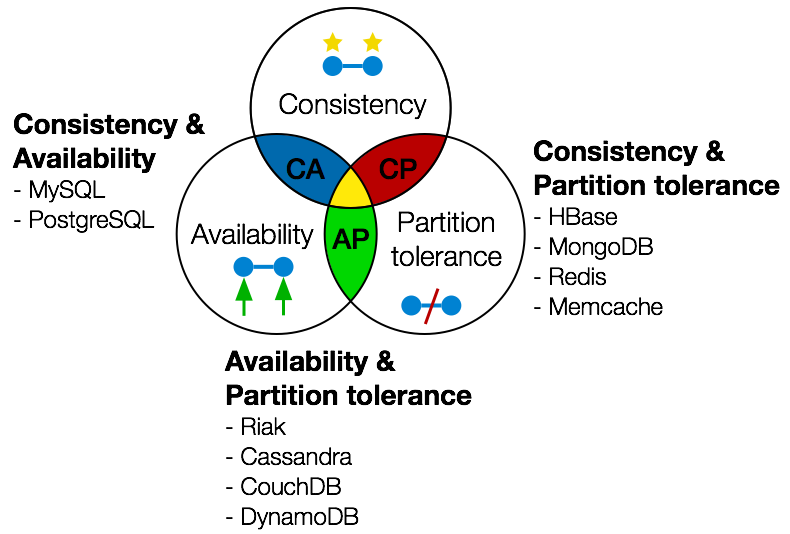
\includegraphics[width=0.9\textwidth]{gfx/CAPTheorem.png}
  \caption{\label{fig:captheorem}Clasificación de bases de datos mediante el teorema de CAP.}
\end{figure}

\section{Tipos de bases de datos NoSQL}

En esta sección vamos a caracterizar las bases de datos NoSQL según la forma en la que almacenan los datos. Podemos clasificar la mayoría de bases de datos NoSQL en alguna de las siguientes 4 categorías, como se describe en la propia documentación de MongoDB \cite{mongoclassification}.

\begin{itemize}
    \item \texttt{Almacenamiento clave-valor}: Son grandes tablas que almacenan la información en forma de clave-valor. Las bases de datos de este tipo más populares son: RedisDB, Riak y Voldemort.
    \item \texttt{Almacenamiento basado en documentos}: Es este tipo de bases de datos, los datos se almacenan en forma de documentos. El concepto de documento depende de la definición de la base de datos, normalmente son grandes conjuntos de claves-valor codificados o encapsulados como un tipo de documento. En esta categoría, MongoDB es el más popular y más usado, pero existen otros como CouchDB.
    \item \texttt{Almacenamiento basado en grafos}: Estas bases de datos almacenan relaciones en forma de grafos. Algunas de las bases de datos más populares son: Neo4j y FlockDB.
    \item \texttt{Almacenamiento en columnas}: En este tipo de bases de datos, se almacenan columnas en lugar de filas como en el resto de tipos. Está optimizado para grandes volúmenes de datos. Las bases de datos más populares de este tipo son: Cassandra y HBase. 
\end{itemize}

En el artículo \cite{nosqlcomparativas}, puede verse una comparativa entre distintas bases de datos NoSQL sobre lenguaje en el que están escritas, ternologías que utilizan, tipo de base de datos, etc.

\section{Comparativa NoSQL con SGBDR}

En esta sección vamos a realizar una comparativa entre las bases de datos SQL y NoSQL.

En primer lugar, además de las dos diferencias comentadas anteriormente, es de destacar, que las bases de datos NoSQL son libres de esquema, esto es, que no necesitan una planificación antes de empezar a almacenar datos a nivel de relaciones, tablas, etc. Los datos almacenados son independientes entre ellos y pueden ser totalmente distintos. Esto aporta un gran valor en el sentido de adaptabilidad a nuevos cambios.

\subsection{Sistemas de Gestión de Bases de Datos Relacionales}

Vamos a dar algunas características que caracterizan a Sistemas de Gestión de Bases de Datos Relacionales (SGBDR), para comenzar veremos algunos de las ventajas que presentan de este tipo de base de datos:

\begin{itemize}
    \item Mayor soporte y herramientas debido a su amplia presencia en el mercado.
    \item Permiten combinar diferentes tablas eficientemente para obtener información relacionada.
    \item Los datos siguen una estructura predefinida en los esquemas.
    \item Proporcionan atomicidad en las operaciones y transaccionalidad entre tablas, esto evita que queden datos inconsistentes si se produce un error en cualquier punto de una operación.
\end{itemize}

Como inconvenientes señalar:

\begin{itemize}
    \item No son flexibles, en el sentido de que los datos tienen que seguir el esquema definido y tienen que estar correctamente validados.
    \item Incremento del procesamiento con el incremento de la complejidad en las relaciones.
    \item Dificultad para escalar, habitualmente necesitan de ampliaciones costosas de hardware.
\end{itemize}

\subsection{Bases de Datos NoSQL}

Una de las principales características que tendría el conjunto de bases de datos NoSQL, es que proporcionan una manera alternativa de almacenar la información y muy diversa por los tipos que comentamos anteriormente, por tanto, ya nos proporcionan una cierta ventaja de flexibilidad que no tenemos con los sistemas SGBDR tradicionales. Veamos ahora algunas características favorables que poseen las bases de datos NoSQL:

\begin{itemize}
    \item Escalabilidad. En general, tienen buen escalamiento horizontal.
    \item Soporte para modelos flexibles, libres de esquemas, tipos y validaciones.
    \item Optimizadas para grandes volúmenes de datos.
    \item Precisan de menos recursos para su funcionamiento.
\end{itemize}

Por contra:

\begin{itemize}
    \item No todas garantizan la atomicidad y consistencia en los datos.
    \item Falta de estandarización. No existe lenguaje un estándar para estas bases de datos, al contrario que ocurre con las BD Relacionales que todas usan SQL.
    \item Falta de herramientas de gestión. Muchas de ellas solo son accesibles por consola.
\end{itemize}

\section{MongoDB}

En esta sección vamos a centrarnos en la base de datos NoSQL más popular hasta el momento, MongoDB es una base de datos orientada a documentos muy usada para técnicas de Big Data. Toda esta sección está extraida de la documentación oficial de MongoDB \cite{mongodb}.

Las principales características son:

\begin{itemize}
    \item MongoDB es una base de datos \textit{open source}, escrita en C++, lo que favorece su rapidez y le proporciona un buen rendimiento.
    \item Es una base de datos distribuida en su núcleo, por lo que se escala horizontalmente de forma fácil, permite la distribución geográfica y una alta disponibilidad.
    \item Almacenamiento de modelo de datos flexibles. Basada en documentos en forma de JSON, permite indexación y operaciones de agregación.
    \item Garantiza transacciones ACID (atomicidad, consistencia, aislamiento y durabilidad) en multidocumentos. Esta reciente característica ha sido integrada en la versión 4.0 de MongoDB.
\end{itemize}

\subsection{Modelo de datos}\label{datamodelmongo}

MongoDB nos provee de un modelo de datos flexible, esto nos permite almacenar desde un documento simple de parejas clave-valor, hasta un documento con subdocumentos embebidos y/o arrays complejos a varios niveles de profundidad.

Posee una sintaxis para realizar consultas muy variada, nos permite hacer consultas simples, con un lenguaje muy descriptivo, sofisticados \textit{pipeline} para consulta, transformación y explotación de datos, búsquedas facetadas, etc.

MongoDB almacena los datos en formato BSON \cite{bsonspec} que es una extensión de los objetos nativos de JavaScript (JSON) a los que añade algunos tipos de datos extra. Estos tipos de datos, se asemejan a los objetos que encontramos en los distintos lenguajes de programación, lo que hace que se produzca una rápida adaptación y una fácil integración con el modelo de datos de MongoDB.

Una de las principales diferencias con las bases de datos relacionales a la hora de modelizar, es que, mientras que en las bases de datos relaciones es habitual crear distintas tablas para trabajar mediante JOINs, en MongoDB es habitual tener todos los datos necesarios para un registro en un mismo documento, lo que reduce la complejidad de tener que realizar JOINs entre tablas y ayuda a la mejora del rendimiento de las consultas.

\subsection{Tipos de consultas}

MongoDB tiene distintos métodos para la consulta y explotación de los datos almacenados:

\begin{itemize}
    \item Clave-valor: Búsquedas simples en cualquier campo del documento.
    \item Rangos: Es posible utilizar los operadores de desigualdades (mayor que, menor que...) para hacer búsquedas por rango y obtener un subconjunto de documentos que satisfagan las condiciones.
    \item Búsquedas Geoespaciales: Devuelven resultados basados en proximidad a ciertos criterios.
    \item Búsquedas de resutlados en un orden relevante, o en búsquedas facetadas. Es posible utilizar operadores lógicos (and, or...), agrupar, contar resultados, etc.
    \item Operadores de agregación: Permite hacer consultas y transformaciones de los datos almacenados. Provee una interfaz completa de operadores dedicados (operaciones lógicas, desigualdades, proyecciones...). En este trabajo, veremos la implementación de consultas de bases de conjuntos difusos sobre este operador de agregación.
    \item JOINs y grafos: con el operador \textit{lookup} podemos hacer JOIN entre colecciones, y con el operador \textit{graphLookup} mongo provee una forma nativa de procesar grafos, árboles y estructuras jerárquicas.
\end{itemize}


\subsection{Indexación}

Según se define en la propia documentación de MongoDB \cite{mongodb}, <<\textit{la indexación es un mecanismo crucial para la optimización del rendimiento y escalabilidad del sistema mientras provee un acceso flexible a tus datos}>>. Mongo permite la indexación en cualquier campo del documento, incluso en los campos de un array.

Mongo provee la facilidad para crear índices compuestos, únicos, array, índices geoespaciales, hash y texto.

Además, la intersección de índices permite a MongoDB usar más de un índice para la optimización de las consultas.

\subsection{Agregación}

Una de las características más importantes de MongoDB a la hora de explotar y transformar datos son las agregaciones. Esta base de datos nos provee dos formas de realizarla, mediante \textit{map-reduce} y mediante \textit{pipeline}.

\subsubsection{Map-Reduce}\label{mapreduce}

Map-Reduce es un modelo de programación general muy utilizado para trabajar con grandes volúmenes de datos y poder introducir paralelismo. MongoDB provee un comando para utilizarlo directamente sobre la base de datos de forma nativa.

El modelo map-reduce, consiste en generar un subconjunto de documentos útiles preprocesando un conjunto más amplio previamente y agrupando en una última etapa. Puede encontrarse más información de este comando y sus usos en \href{https://docs.mongodb.com/manual/core/map-reduce/}{la documentación oficial}.

\subsubsection{Pipeline}\label{pipeline}

La segunda forma para implementar operaciones de agregación es mediante el framework \textit{pipeline}. Con este comando los documentos son procesados mediante una secuencia ordenada de etapas, donde cada etapa recibe una colección de documentos procesados por la etapa anterior, los procesa y los envía como entrada de la siguiente etapa, así hasta producir el resultado final. Mediante este operador, el filtrado de documentos sobre una colección de documentos se haría usando el operador \textit{match} en la etapa correspondiente del \textit{pipeline} de agregación.

Las etapas permitidas para este operador se pueden encontrar en la \href{https://docs.mongodb.com/manual/reference/operator/aggregation-pipeline/}{documentación del operador}. En nuestra propuesta se proporciona una serie de operadores adicionales que se pueden utilizar en las etapas de \textit{match} y \textit{projection}.

La etapa \textbf{match}, como se describe en su propia documentación, sirve para filtrar los documentos que van a pasar a la siguiente etapa. Selecciona aquellos que cumplan ciertas condiciones descritas mediante los operadores\footnote{https://docs.mongodb.com/manual/reference/operator/aggregation/} permitidos para esta etapa. Los operadores que hemos extendido para trabajar con datos difusos son:

\begin{itemize}\label{mongooperators}
    \item \textbf{\$eq}: selecciona los documentos cuyo valor coincida con el especificado.
    \item \textbf{\$gt}: selecciona los documentos cuyo valor sea mayor que el especificado.
    \item \textbf{\$gte}: selecciona los documentos cuyo valor sea mayor o igual que el especificado.
    \item \textbf{\$lt}: selecciona los documentos cuyo valor sea menor que el especificado.
    \item \textbf{\$lte}: selecciona los documentos cuyo valor sea menor o igual que el especificado.
\end{itemize}

Además de estos, vamos a ver los que nos serán de utilidad para su implementación:

\begin{itemize}
    \item \textbf{\$and}: Operador lógico, recibe una lista de expresión y filtra aquellos documentos que cumplan con todas ellas.
    \item \textbf{\$or}: Operador lógico, recibe una lista de expresión y filtra aquellos documentos que cumplan al menos una de ellas.
    \item \textbf{\$add}: Operador aritmético, recibe una lista de expresiones, que deben de ser evaluadas como un número, y suma todas ellas.
    \item \textbf{\$substract}: Operador aritmético, recibe una lista de expresiones, que deben de ser evaluadas como un número, y resta todas ellas.
    \item \textbf{\$multiply}: Operador aritmético, recibe una lista de expresiones, que deben de ser evaluadas como un número, y multiplica todas ellas.
    \item \textbf{\$divide}: Operador binario aritmético, recibe una lista de 2 expresiones y devuelve la división del primero de ellos entre el segundo.
    \item \textbf{\$cond}: Operador ternario condicional, recibe una lista de 3 expresiones y permite evalua la segunda o la tercera en función del resultado obtenido en la primera. Este operador nos permite realizar los clásicos \textit{if-else} de cualquier lenguaje de programación.
    \item \textbf{\$arrayElemAt}: Operador para expresiones con arrays. Recibe una lista de 2 expresiones, donde el primer parámetro es el campo que corresponde con el array y la segunda es el índice del array que se quiere obtener. Devuelve el valor que se encuentre en la posición solicitada del array.
    \item \textbf{\$expr}\footnote{\url{https://docs.mongodb.com/manual/reference/operator/query/expr/}}: El operador ``expr'' es un operador de consultas, permite el uso\footnote{Uso de operador expr con expresiones condicionales: \url{https://docs.mongodb.com/manual/reference/operator/query/expr/\#using-expr-with-conditional-statements}} de expresiones de agregación en el lenguaje de consultas. El uso que nos interesa es el combinado con el operador ``\$cond''.
\end{itemize}

La etapa \textbf{projection} sirve para establecer que campos mostrar de la colección resultante. Nos permite tanto eliminar campos del propio documento, como generar y visualizar campos nuevos. En esta parte nos hemos centrado en ampliar la posibilidad de proyectar el grado de cumplimiento para los campos difusos.

En el capítulo \ref{propuesta} veremos estos operadores y la propuesta realizada para ampliar estas etapas.


\chapter{Conjuntos Difusos}
En este capítulo, haremos una introducción a la teoría de conjuntos difusos. Veremos qué son y las principales operaciones con estos conjuntos. Esta permite nos permite modelar matemáticamente información imperfecta, que es usada frecuentemente por los humanos en su comunicación y razonamiento.

Vamos a ver que bases de datos difusas existen y sus principales características para adentrarnos en el mundo de la representación difusa en base de datos. El objetivo de esta es dotar a los sistemas automáticos de una poderosa forma de toma de decisiones, similares a las que tomamos las personas, basada en información que no pretende ser del todo exacta.

Por último, terminaremos el capítulo definiendo los operadores difusos que utilizaremos en nuestra propuesta en el capítulo \ref{propuesta}.

\section{Teoría de conjuntos difusa}

La principal teoría para hablar de datos imprecisos fue introducida por L.A Zadeh \cite{fuzzysetszadeh} en 1965. Vamos a basarnos en ella para explicar los conjuntos difusos.

La teoría de conjuntos difusos (\textit{fuzzy sets}) hace una generalización de la teoría de conjuntos clásica, en la que se define un conjunto como un grupo de elementos que pertenecen o no a este conjunto. En la teoría de conjuntos difusa, se añade un elemento más a tener en cuenta, el grado de pertenencia al conjunto, esto es, cada elemento pertenece a un conjunto con un grado de pertenencia determinado que suele representarse con un número $x \in [0,1]$. Haciendo una analogía, en la teoría de conjuntos clásica, los elementos pertenecen con solo dos posibles valores $0$ ó $1$, que indicarían si pertenece o no al conjunto.

Basándonos en los descrito anteriormente, vamos a dar una definición de conjunto difuso.

\begin{definition}[Conjunto difuso]
Sea $\Omega$ un dominio (de objetos), denotemos a los elementos de $\Omega$ por $x$. Sea $f: \Omega \longrightarrow [0,1]$ una función. Definimos un \textbf{conjunto difuso} $F$ como:

\begin{equation*}
    F = \left\{ f(x)/x \enspace | \enspace x\in\Omega, f(x) \in [0,1] \right\}
\end{equation*}
\end{definition}

Es común no dar una lista exhaustiva de elementos del conjunto difuso, basta con dar una definición de la función $f$, a la que denominamos \textbf{función de pertenencia}.

Estos conceptos suelen ser muy subjetivos y en la práctica, suelen depender del contexto en el que se encuentren, esto es, un mismo valor, depende del contexto, puede pertenecer a un conjunto u otro. Veamos un mismo ejemplo en dos contextos distintos para ilustrarlo, aprovecharemos el ejemplo para afianzar la definición de conjunto difuso.

\begin{example}
Supongamos que tenemos los datos de la tabla \ref{datatable} con la altura de 5 personas:

\begin{table}[h]
\centering
\begin{tabular}{|l|l|}
\hline
\textbf{Nombre} & \textbf{Altura} \\ \hline
Juan            & 175             \\ \hline
Pepe            & 195             \\ \hline
Marco           & 170             \\ \hline
Felipe          & 180             \\ \hline
Antonio         & 185             \\ \hline
\end{tabular}
\caption{Datos de altura}
\label{datatable}
\end{table}

Vamos a definir el conjunto difuso que representa a los jugadores \textit{altos} en dos deportes distintos:

Supongamos como primer deporte el baloncesto, y podríamos tener una estimación del conjunto difuso como sigue:

\begin{equation*}
    altos = \{ \num{0.8}/195, \num{0.3}/180, \num{0.35}/185\}
\end{equation*}

sin embargo, para un deporte como el fútbol, podríamos tener el siguiente conjunto:

\begin{equation*}
    altos = \{\num{0.2}/175, \num{0.1}/170, 1/195, \num{0.7}/180, \num{0.82}/185\}
\end{equation*}

\end{example}

Aprovechando el ejemplo previo, vamos a introducir un nuevo concepto:

\begin{definition}[Etiqueta lingüística]
Llamamos \textbf{etiqueta lingüística} a aquella palabra en lenguaje natural que describe un conjunto difuso.
\end{definition}

\subsection{Conceptos sobre conjuntos difusos}

Similar a los conceptos de la teoría clásica de conjuntos, vamos a dar una introducción a los conceptos sobre conceptos difusos, veremos como todos ellos dependen de la función de pertenencia.

Sean $\Omega$ un dominio, y sean $F_1$ y $F_2$ dos conjuntos difusos con $f_1$ y $f_2$ sus funciones de pertenencia, respectivamente. Entonces, se tiene:

\begin{itemize}
    \item $F_1$ y $F_2$ son \textbf{iguales} si, y solo si, las funciones de pertenencia son iguales. Esto es, $F_1 = F_2 \Leftrightarrow f_1(x) = f_2(x) \quad \forall x \in \Omega$.
    \item $F_1$ está \textbf{incluido} en $F_2$ si, y solo si, $f_1$ es menor o igual que $f_2$. Esto es, $F_1 \subseteq F_2 \Leftrightarrow f_1(x) \leq f_2(x) \quad \forall x \in \Omega$.
    \item Se define el \textbf{soporte} de $F_1$ como el subconjunto de valores de $\Omega$ tal que la función de pertenencia es mayor que cero. Esto es, $sop(F_1) = \{ x \in \Omega \enspace | \enspace f_1(x) > 0 \}$
    \item Se define el \textbf{$\alpha$-corte} de $F_{1_\alpha}$ como el subconjunto de $\Omega$ tal que la función de pertenencia es mayor o igual que un valor dado, $\alpha$. Esto es, $F_{1_\alpha} = \{ x \in \Omega \enspace | \enspace f_1(x) \geq \alpha \}$.
    \item Se define el \textbf{núcleo} de $F_1$ como el subconjunto de $\Omega$ tal que el grado de pertenencia es 1. Esto es, $ker(F_1) = \{ x\in \Omega \enspace | \enspace f_1(x) = 1 \}$.
    \item Se define la \textbf{altura} de $F_1$ como el supremo de todos los grados de pertenencia. Esto es, $hgt(F_1) = \sup_{x\in \Omega} f_1(x)$.
    \item Se dice que un conjunto $F_1$ difuso está \textbf{normalizado} si, y solo si, la altura es igual a 1. Esto es, $\exists x \in \Omega$ tal que $f_1(x) = 1$.
\end{itemize}

\subsection{Números difusos}\label{fuzzynumbers}

Los números difusos fueron introducidos por Zadeh \cite{fuzzynumberszadeh} para poder trabajar con información imprecisa de forma práctica, posteriormente, otros trabajos han ido refinando y redefiniendo este concepto. En esta sección, vamos a definirlos y vamos a ver cómo trabajar con ellos. Es una sección muy importante para nuestro trabajo, ya que será con números difusos como representaremos la información en la base de datos. 

\begin{definition}[Número difuso]
Sea $F$ un conjunto difuso en $\Omega$ con $f$ su función de pertenencia. Diremos que $F$ es un \textbf{número difuso} si cumple:

\begin{enumerate}
    \item $f$ es convexa
    \item $f$ es semi-continua superiormente
    \item El soporte de $F$ está acotado 
\end{enumerate}
\end{definition}

Veamos ahora la forma general de un número difuso. Sea $\Omega$ un dominio ordenado y sean $\alpha, \beta, \gamma, \delta \in \Omega$ con $\alpha \leq \beta \leq \gamma \leq \delta$, entonces la \textbf{forma de pertenencia general de un número difuso} es:

\begin{equation*}
    f(x) = \left\{ { \begin{array}{cc}
                    0 & x < \alpha \\ 
                    r(x) & x\in [\alpha,\beta) \\
                    h & x\in [\beta,\gamma] \\
                    s(x) & x\in (\gamma,\delta] \\
                    0 & x > \delta \\ 
                    \end{array}  } \right.
\end{equation*}

donde $r: \Omega \longrightarrow [0,1]$ es no decreciente, $s: \Omega \longrightarrow [0,1]$ es no creciente y $h \in (0,1]$ con $r(\beta) = h = s(\gamma)$. Véase la figura \ref{fig:generaltrapezoid}.

\begin{figure}[h]
  \centering
  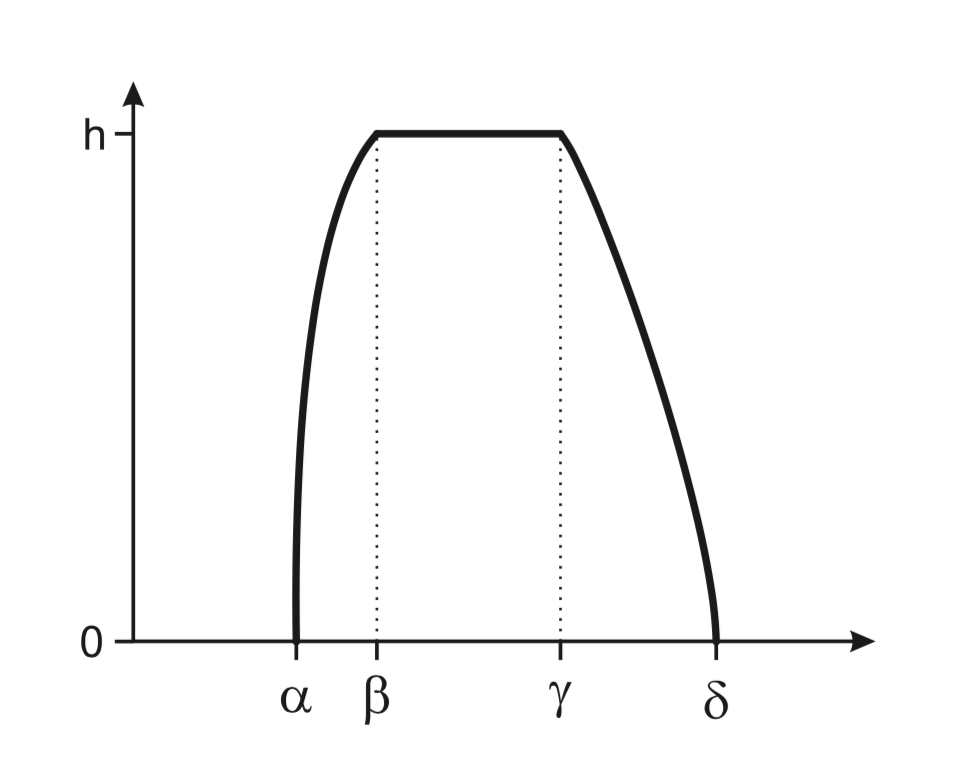
\includegraphics[width=0.9\textwidth]{gfx/fuzzynumber.png}
  \caption{\label{fig:generaltrapezoid}Número difuso generalizado.}
\end{figure}

Los números difusos que nos interesan a nosotros especialmente, y que utilizaremos para dar nuestra solución, son aquellos en los que las funciones $r$ y $s$ son lineales. Estos son llamados los \textbf{trapezoides}, veáse figura \ref{fig:trapezoid}, y tienen la siguiente forma de pertenencia de número difuso.

\begin{equation}\label{trapezoidrepresentation}
    f(x) = \left\{ { \begin{array}{cc}
                    0 & x < \alpha \\ 
                    h + \frac{(x-\beta)h}{\beta-\alpha} & x\in [\alpha,\beta) \\
                    h & x\in [\beta,\gamma] \\
                    h + \frac{(x-\gamma)h}{\delta-\gamma} & x\in (\gamma,\delta] \\
                    0 & x > \delta \\ 
                    \end{array}  } \right.
\end{equation}

\begin{figure}[h]
  \centering
  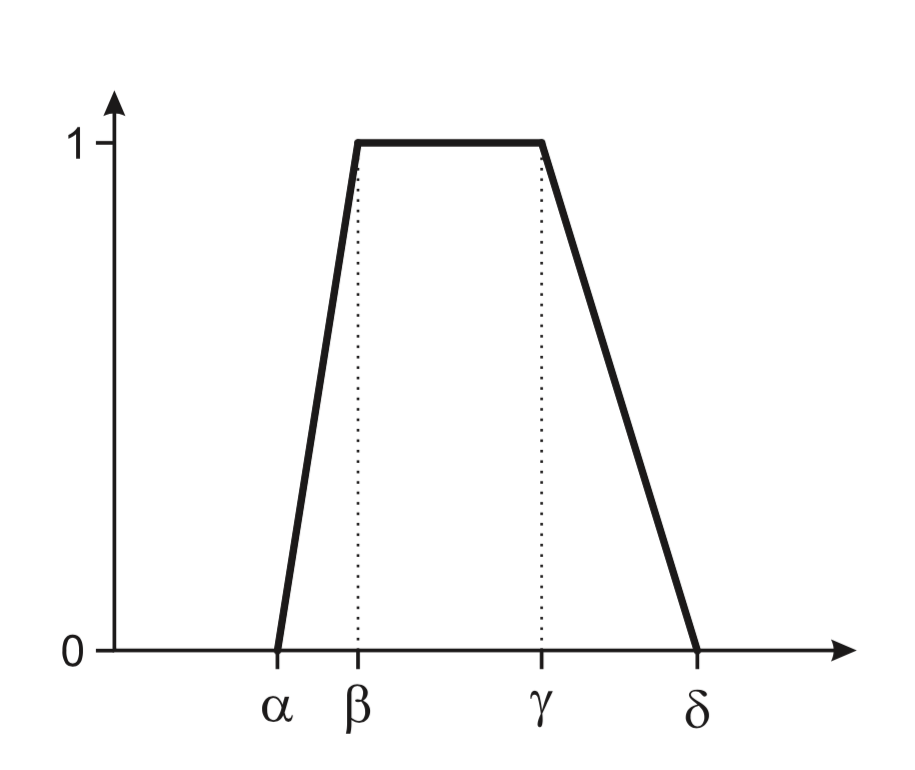
\includegraphics[width=0.9\textwidth]{gfx/trapezoid.png}
  \caption{\label{fig:trapezoid}Número difuso trapezoidal.}
\end{figure}

Además, habitualmente estará normalizado ($h=1$) y por tanto nos basta con una tupla $(\alpha, \beta, \gamma, \delta)$ para definir un número difuso.

\begin{remark}\label{notaciontrapezoide}
Notemos que esta representación nos vale incluso cuando se tengan solo 1,2 ó 3 valores. Estos serán llamados \textit{crisp}, \textit{intervalo} y \textit{triangulares} respectivamente. Con un valor $a$, tendremos $\alpha = \beta = \gamma = \delta = a$, con dos valores, $a,b$ tendremos $\alpha = \beta = a$ y $\gamma = \delta = b$ y con tres valores, $a,b,c$ tendremos $\beta = \gamma = b$. Veáse un ejemplo de ello para el caso triangular en \ref{fig:trapezoid3}
\end{remark}

\begin{figure}[h]
  \centering
  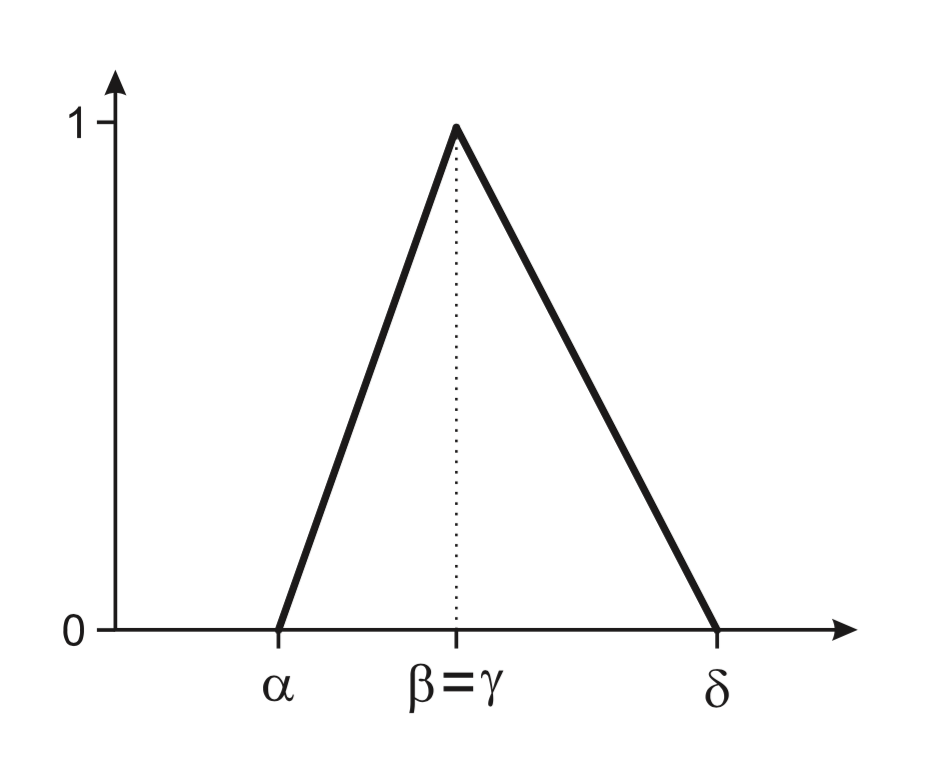
\includegraphics[width=0.9\textwidth]{gfx/trapezoid3.png}
  \caption{\label{fig:trapezoid3}Trapezoide con 3 valores.}
\end{figure}

\section{Información Imprecisa en bases de datos}

Vamos a introducir los precedentes existentes en el área de representación y tratamiento de información imprecisa en bases de datos. Se pueden encontrar referencias de un amplio abanico para dar solución al desafío que nos enfrentamos.

Además, el término ``imprecisa'', referida a la información, engloba varios significados que podemos distinguir \cite{fuzzynotion}:

\begin{itemize}
    \item Incompletitud: Información incompleta, es decir, no tenemos toda la información posible.
    \item Incertidumbre: No se sabe si la información es cierta o no.
    \item Desconocimiento: No se tiene información.
    \item Inaplicabilidad: La información de la que se dispone no es aplicable a ninguna entidad.
\end{itemize}

Podemos clasificar los distintos tipos de modelos en dos categorías según el uso o no de la lógica difusa. Dentro de las propuestas que utilizan lógica difusa, nos centraremos en el modelo GEFRED, en el que nos hemos basado para realizar la propuesta sobre MongoDB. Podemos obtener una visión conjunta de todas las propuestas que se van a mencionar a lo largo de esta sección en \cite{tesismedina, tesisbarranco, tesispepe}.

\subsection{Aproximaciones sin emplear lógica difusa}

Vamos a resumir las distintas propuestas que se han realizado sin utilizar la teoría de conjuntos difusos vista en este mismo capítulo, agrupadas por la técnica utilizada para llevar a cabo el propósito:

\begin{itemize}
    \item \textbf{Valores nulos}: E. Codd realizó la primera propuesta en \cite{codd} y fue evolucionándola en \cite{codd1, codd2, codd3}. Consiste en utilizar el valor \texttt{NULL} en todo el dominio disponible de la base de datos. Este valor indicaba que no se conocía el valor del atributo.
    \item \textbf{Valores por defecto}: Esta propuesta, publicada en \cite{date} surge por la idea del autor de que los valores nulos no habían sido tratados correctamente, y propone sustituirlos por un valor por defecto del dominio. Así, en caso de no conocer la información de un atributo, se asignaría el valor por defecto seleccionado para dicho atributo.
    \item \textbf{Rangos de valores}: Propuesta realizada por Grant en \cite{grant}, realizó una extensión del modelo relacional para almacenar un rango de valores posibles y la redefinición de los operadores para que en su evaluación se pudiese obtener el rango de valores \textit{verdadero}, \textit{falso} y \textit{quizás}.
     \item \textbf{Bases de datos estadísticas y probabilísticas}: En \cite{wong} se da una propuesta de bases de datos estadísticas, esto es, cada consulta resuelve la incertidumbre como un experimento estadístico obtiendo como resultado la tupla que minimice el error estadístico. En \cite{dbprobabilistic} se obtiene una propuesta para base de datos probabilística, asociando probabilidades a los valores de los atributos tratando a cada atributo como una distribución de probabilidad discreta.
\end{itemize}

\subsection{Bases de datos difusas}

Veamos ahora las propuestas que se han realizado para bases de datos utilizando la lógica difusa y teoría de conjuntos difusos. Estas propuestas se centran en añadir a cada tupla un \textit{grado}, normalmente en el intervalo $[0,1]$, a cada tupla.

Las distintas propuestas son las dadas por Buckles y Petry en \cite{buckles, buckles2, buckles3} basado en el concepto de relación de similitud, Prade y Testemale en \cite{prade, prade2, prade3, prade4} basada en la teoría de posibilidad, Umano y Fukami en \cite{fukami, fukami2, fukami3, fukami4} basado también en la teoría de la posibilidad, el modelo propuesto por Zemankova y Kaendel en \cite{zemankova, zemankova2} que realiza una representación imperfecta similar a los modelos posibilísticos, pero que adicionalmente desarrolla un lenguaje de manipulación de datos que analiza las relaciones entre posibilidad y certeza. Por último, la propuesta de Medina, Pons y Vila \cite{gefred}, el modelo GEFRED, que pretende unificar todas las propuestas anteriores y dar una solución completa al tratamiento de información imprecisa en base de datos relacional, se basa en lo que llaman \textit{Dominio difuso generalizado} y \textit{relación difusa generalizada}, a través de los cuales, GEFRED redefine los operadores del algebra relacional en el llamado \textit{Álgebra relacional difuso generalizado}. No entramos en detalle de estos operadores pues se trata de lenguaje SQL que no utilizaremos en este trabajo, pero puede verse en \cite{gefred}.

\subsection{Operadores difusos}

Para el tratamiento de información difusa, es necesario definir ciertos operadores para poder ejecutar consultas sobre la base de datos. En esta sección veremos los operadores que hemos utilizado para trabajar con esta información y el cómo obtener cada uno de ellos.

Cuando queremos comparar dos atributos difusos de una base de datos, dotamos a los valores de un grado de cumplimiento, al que llamaremos \textbf{cdeg}. Este grado de depende de la medida de posibilidad que estemos utilizando, en nuestro caso, vamos a considerar dos medidas de posibilidad distintas, las que llamaremos como \textit{necesidad} y \textit{posibilidad}.

\subsubsection{Operadores de igualdad difusos}

Sean $A$ y $B$ dos distribuciones de posibilidad trapezoidales, y sean $f_A$ y $f_B$ sus funciones de pertenencia, respectivamente, definidas sobre un dominio ordenado $\Omega$. Para calcular el grado de igualdad dependiendo de la medida, utilizamos las siguientes definiciones \cite{tesispepe}:

\begin{definition}[Operador FEQ]
Para comparar ambas distribuciones y obtener el grado de compatibilidad entre ellas, esto es, en qué medida son \texttt{posiblemente} iguales, se usa la ecuación:

\begin{equation}
    feq(A,B) = \sup_{x \in \Omega} \min (f_A(x), f_B(x))
\end{equation}
\end{definition}

\begin{definition}[Operador NFEQ]
Para comparar ambas distribuciones y obtener el grado de compatibilidad entre ellas, esto es, en qué medida son \texttt{necesariamente} iguales, se usa la ecuación:

\begin{equation}
    nfeq(A,B) = \inf_{x \in \Omega} \max (1-f_A(x), f_B(x))
\end{equation}
\end{definition}


\subsubsection{Operadores relacionales difusos}

Sean $A$ y $B$ dos distribuciones de posibilidad trapezoidales definidas sobre un dominio ordenado $\Omega$, con $A = \trapezoidA$ y $B=\trapezoidB$. Para calcular el grado de relación dependiendo de la medida, utilizamos las siguientes definiciones \cite{tesispepe}:

\begin{definition}[Operador FGT]
Para obtener el grado en que $A$ es \texttt{posiblemente} mayor que $B$, se usa la ecuación:

\begin{equation}
    fgt(A,B) = \left\{ { \begin{array}{ll}
                    1 & \text{si}\, \gamma_A \geq \delta_B \\ 
                    \frac{\delta_A - \gamma_B}{(\delta_B - \gamma_B)-(\gamma_A - \delta_A)} & \text{si}\, \gamma_A < \delta_B \, \text{y} \, \delta_A > \gamma_B \\
                    0 & \text{en otro caso} \\ 
                    \end{array}  } \right.
\end{equation}
\end{definition}

\begin{definition}[Operador NFGT]
Para obtener el grado en que $A$ es \texttt{necesariamente} mayor que $B$, se usa la ecuación:

\begin{equation}
    nfgt(A,B) = \left\{ { \begin{array}{ll}
                    1 & \text{si}\, \alpha_A \geq \delta_B \\ 
                    \frac{\beta_A - \gamma_B}{(\delta_B - \gamma_B)-(\alpha_A - \beta_A)} & \text{si}\, \alpha_A < \delta_B \, \text{y} \, \beta_A > \gamma_B \\
                    0 & \text{en otro caso} \\ 
                    \end{array}  } \right.
\end{equation}
\end{definition}

\begin{definition}[Operador FGTE]
Para obtener el grado en que $A$ es \texttt{posiblemente} mayor o igual que $B$, se usa la ecuación:

\begin{equation}
    fgte(A,B) = \left\{ { \begin{array}{ll}
                    1 & \text{si}\, \gamma_A \geq \beta_B \\ 
                    \frac{\delta_A - \alpha_B}{(\beta_B - \alpha_B)-(\gamma_A - \delta_A)} & \text{si}\, \gamma_A < \beta_B \, \text{y} \, \delta_A > \alpha_B \\
                    0 & \text{en otro caso} \\ 
                    \end{array}  } \right.
\end{equation}
\end{definition}

\begin{definition}[Operador NFGTE]
Para obtener el grado en que $A$ es \texttt{necesariamente} mayor o igual que $B$, se usa la ecuación:

\begin{equation}
    nfgte(A,B) = \left\{ { \begin{array}{ll}
                    1 & \text{si}\, \alpha_A \geq \beta_B \\ 
                    \frac{\beta_A - \alpha_B}{(\beta_B - \alpha_B)-(\alpha_A - \beta_A)} & \text{si}\, \alpha_A < \beta_B \, \text{y} \, \beta_A > \alpha_B \\
                    0 & \text{en otro caso} \\ 
                    \end{array}  } \right.
\end{equation}
\end{definition}

\begin{definition}[Operador FLT]
Para obtener el grado en que $A$ es \texttt{posiblemente} menor que $B$, se usa la ecuación:

\begin{equation}
    flt(A,B) = \left\{ { \begin{array}{ll}
                    1 & \text{si}\, \beta_A \leq \alpha_B \\ 
                    \frac{\alpha_A - \beta_B}{(\alpha_B - \beta_B)-(\beta_A - \alpha_A)} & \text{si}\, \beta_A > \alpha_B \, \text{y} \, \alpha_A < \beta_B \\
                    0 & \text{en otro caso} \\ 
                    \end{array}  } \right.
\end{equation}
\end{definition}

\begin{definition}[Operador NFLT]
Para obtener el grado en que $A$ es \texttt{necesariamente} menor que $B$, se usa la ecuación:

\begin{equation}
    nflt(A,B) = \left\{ { \begin{array}{ll}
                    1 & \text{si}\, \delta_A \leq \alpha_B \\ 
                    \frac{\gamma_A - \beta_B}{(\alpha_B - \beta_B)-(\delta_A - \gamma_A)} & \text{si}\, \delta_A > \alpha_B \, \text{y} \, \gamma_A < \beta_B \\
                    0 & \text{en otro caso} \\ 
                    \end{array}  } \right.
\end{equation}
\end{definition}

\begin{definition}[Operador FLTE]
Para obtener el grado en que $A$ es \texttt{posiblemente} menor o igual que $B$, se usa la ecuación:

\begin{equation}
    flte(A,B) = \left\{ { \begin{array}{ll}
                    1 & \text{si}\, \beta_A \leq \gamma_B \\ 
                    \frac{\delta_B - \alpha_A}{(\beta_A-\alpha_A)-(\gamma_B - \delta_B)} & \text{si}\, \beta_A > \gamma_B \, \text{y} \, \alpha_A < \delta_B \\
                    0 & \text{en otro caso} \\ 
                    \end{array}  } \right.
\end{equation}
\end{definition}

\begin{definition}[Operador NFLTE]
Para obtener el grado en que $A$ es \texttt{necesariamente} menor o igual que $B$, se usa la ecuación:

\begin{equation}
    nflte(A,B) = \left\{ { \begin{array}{ll}
                    1 & \text{si}\, \delta_A \leq \gamma_B \\ 
                    \frac{\gamma_A - \delta_B}{(\gamma_B - \delta_B)-(\delta_A - \gamma_A)} & \text{si}\, \delta_A > \gamma_B \, \text{y} \, \gamma_A < \delta_B \\
                    0 & \text{en otro caso} \\ 
                    \end{array}  } \right.
\end{equation}
\end{definition}


\chapter{Propuesta difusa en MongoDB}
\label{propuesta}
Una vez introducida la teoría de conjuntos difusos en el capítulo previo y de dar una introducción a las bases de datos no relacionales, vamos a realizar una propuesta para la base de datos NoSQL, MongoDB, para dotarla de capacidad para la el manejo de datos difusos.

En la literatura podemos encontrar trabajos con propuestas para bases de datos NoSQL, véase \cite{fuzzyquerygraph, fuzzyquerygraph2, fuzzyquerygraph3}, donde se pueden encontrar propuestas para bases de datos basadas en grafos o \cite{fuzzyqueryhbase} donde se habla de modelado de conjuntos difusos en la base de datos HBase. En \cite{fuzzyquerymongo} podemos encontrar una propuesta para realizar consultas difusas en la base de datos MongoDB, el cuál hemos utilizado para sacar algunas ideas sobre las que se basan nuestra propuesta.

El objetivo de la propuesta que se presenta en este trabajo es mantener la compatibilidad con el funcionamiento estándar de MongoDB, mediante el uso del lenguaje proporcionado y de los mecanismos para representar datos que éste proporciona, para representar los tipos de datos difusos considerados e implementar los mecanismos para la elaboración de las consultas difusas sobre los mismos.

\section{Representación de información en MongoDB}

Dependiendo del tipo de dato, acordamos su representación como sigue:

\begin{itemize}
    \item Datos precisos: Hacen referencia a los datos comunes de MongoDB, enteros, fechas, cadenas de texto, arrays, documentos... Estos datos se seguirán representando con el tipo de dato correspondiente y se trabajará con ellos de forma nativa.
    \item Datos difusos: Como ya adelantamos en los capítulos previos, la forma de trabajar con datos difusos que hemos utilizado es mediante los números difusos \ref{fuzzynumbers} de tipo \textbf{trapezoides} \ref{trapezoidrepresentation}. Para representar esto en MongoDB hemos utilizado \texttt{arrays} con cuatro elementos de tipo numérico.
\end{itemize}

\begin{example}
Vamos a introducir una colección que nos valdrá de ejemplo a lo largo del capítulo para afianzar los conceptos y hacer las demostraciones de las implementaciones que se irán viendo.

El problema que nos planteamos es una base de datos con viviendas. La motivación de este tipo de datos es que algunos de los atributos que utiliza, pueden tratarse fácilmente como difusos, por ejemplo, cuando hablamos del precio o de la superficie de una vivienda, habitualmente en el lenguaje oral es fácil definirlo con un rango de valores o una expresión imprecisa: ``...quiero gastarme entre $110000$€ y $120000$€...'', ``...me gustaría una casa que tenga alrededor de $100m^2$...''.

Un ejemplo de un documento de esta colección quedaría:

\begin{lstlisting}[numbers=none]
{
    _id: ObjectId("5b2501805d492f2c6f51a79e"),
    id_inm: 318.0,
    tipo: "PISO",
    precio: [116625.0, 129218.0, 131771.0, 137828.0],
    habitaciones: [2.0, 2.0, 3.0, 3.0],
    superficie: [60.0, 60.0, 60.0, 60.0],
    descripcion: "* CHURRIANA DE LA VEGA, 60 m2 utiles, 2 habitaciones, 1 bano, cocina amueblada, salon, suelos marmol, ascensor, puerta blindada, climalit, exterior, garaje. Ano 2005. Oportunidad!!! Precio: 129.217,60 euros (21.500.000 pts) Ref. 00232 Inm. Aqaba Tlf. 958 26 53 63 / 669 45 41 76."
}
\end{lstlisting}

donde los campos \texttt{precio},  \texttt{superficie} y \texttt{habitaciones} son campos difusos. Nótese, que para que el campo siempre se represente como un trapezoide de cuatro posiciones, hemos utilizado la notación descrita en \ref{notaciontrapezoide}.
\end{example}

\section{Fuzzy Find}

En \cite{tesismedina} se expuso un módulo para permitir extender la capacidad de un SGBDR clásico para que pueda representar y manipular información imprecisa. En este trabajo se ha realizado una prueba de concepto sobre MongoDB mediante la implementación del comando \textbf{fuzzy\_find}, que nos permitirá realizar consultas sobre una base de datos que contenga datos de tipo difuso.

Para llevar a cabo esto, la utilidad que nos provee MongoDB para \href{https://docs.mongodb.com/manual/tutorial/store-javascript-function-on-server/}{almacenar funciones javascript en el servidor de MongoDB}, nos permite su uso en cualquier contexto javascript.

Consideramos una primera alternativa de implementación para esa función basada en el uso del operador de agregación \texttt{map-reduce} descrito en \ref{mapreduce}, pero tras unas pruebas con una cantidad de datos relativamente grande, no obteníamos el rendimiento que esperábamos, las consultas eran demasiado lentas y descartamos esta opción en favor de utilizar el operador de agregación \texttt{pipeline}, véase la sección \ref{pipeline}. Este operador proporciona más opciones de utilidad para nuestro propósito, nos permite utilizar índices y nos ofrece un rendimiento muy superior a la opción basada en el uso de \texttt{map-reduce}.

\texttt{Fuzzy\_find} es un comando de consulta generalizado, en el sentido de que permite expresar consultas clásicas, véase ejemplo~\ref{example:viviendasqueries}, sin cláusulas difusas, y consultas que combinen cláusulas clásicas con cláusulas difusas. De este modo no solo no pierde la funcionalidad de la que mongo provee inicialmente sino que la extiende.

\subsection{Sintaxis del comando \texttt{fuzzy\_find}}

La cabecera de la función \texttt{fuzzy\_find} es la siguiente:

\begin{verbatim}
fuzzy_find(collection, filter, projection, count_name=null)
\end{verbatim}
%
donde los parámetros son:

\begin{itemize}
    \item \textbf{collection}: Nombre de la colección sobre la que se va a ejecutar la consulta.
    \item \textbf{filter}: JSON con la consulta que se va a realizar. Utiliza el formato estándar de MongoDB para especificar las condiciones sobre los documentos a recuperar, incluyendo todos los operadores estándar junto con los operadores que introducimos en nuestra propuesta destinados a expresar condiciones de consulta difusas. Estos operadores los describiremos en la próxima sección.
    \item \textbf{projection}: JSON para la etapa de proyección. Además de usan el formato estándar de MongoDB incorpora operadores específicos para la visualización de datos difusos.
    \item \textbf{count\_name}: Campo opcional. Si se especifica una cadena de texto se añade la etapa \textit{count}\footnote{\url{https://docs.mongodb.com/manual/reference/operator/aggregation/count/}} para devolver la cantidad de documentos recuperados en lugar de los propios documentos.
\end{itemize}

Veamos la sintaxis propuesta mediante un ejemplo.

\begin{example}\label{example:viviendasqueries}

Supongamos una colección \texttt{viviendas} conteniendo los siguientes documentos:

\begin{lstlisting}[numbers=none]
{
    _id: ObjectId("5b2501805d492f2c6f51a79e"),
    id_inm: 318.0,
    tipo: "PISO",
    precio: [116625.0,129218.0,131771.0,137828.0],
    habitaciones: [2.0,2.0,3.0,3.0],
    superficie: [60.0,60.0,60.0,60.0],
    descripcion: "* CHURRIANA DE LA VEGA, 60 m2 utiles, 2 habitaciones, 1 bano, cocina amueblada, salon, suelos marmol, ascensor, puerta blindada, climalit, exterior, garaje. Ano 2005. Oportunidad!!! Precio: 129.217,60 euros (21.500.000 pts) Ref. 00232 Inm. Aqaba Tlf. 958 26 53 63 / 669 45 41 76."
}
{
    _id: ObjectId("5b2501805d492f2c6f51a79f"),
    id_inm: 319.0,
    tipo: "PAREADO",
    precio: [131760.0,132000.0,136674.0,139381.0],
    habitaciones: [2.0,2.0,3.0,3.0],
    superficie: [75.0,75.0,75.0,75.0],
    descripcion: "* CHURRIANA DE LA VEGA, 75 m2. 2 dormitorios, bano, cocina y salon. Plaza de garaje. Nuevo a estrenar. Buenas calidades. Precio 132.000 euros. Inm. Alhamar Tlf. 958 26 68 90."
}
{
    _id: ObjectId("5b2501805d492f2c6f51a7a0"),
    id_inm: 321.0,
    tipo: "PISO",
    precio: [136568.0,138000.0,138900.0,139268.0],
    habitaciones: [2.0,2.0,3.0,3.0],
    superficie: [78.0,78.0,78.0,78.0],
    descripcion: "* CHURRIANA DE LA VEGA, C/Habana Piso  en construccion de 78 m2,  2 habitaciones,  1 bano, cocina americana, comedor de 21 m2, terraza 6 m2, ,suelos de tarima flotante, pintura lisa, calefaccion totalmente instalada de calor azul.  garaje y trastero, En Construccion, le queda menos de 1 ano. Precio: 138.000,00 euros (22.962.952 pts) Ref:  40323. Inm. Tres Plazas Tlf. 958 25 06 46 / 677 40 97 28."
}
\end{lstlisting}
%
si queremos obtener los documentos que cumplen que el campo \texttt{tipo} es igual a \texttt{``PISO"}, podríamos usar la función \texttt{fuzzy\_find} para ejecutar esa consulta como sigue:
%
\begin{verbatim}
fuzzy_find("viviendas", {tipo: "PISO"}, {})
\end{verbatim}
%
obteniendo el siguiente resultado:
%
\begin{lstlisting}[numbers=none]
{
    _id: ObjectId("5b2501805d492f2c6f51a79e"),
    id_inm: 318.0,
    tipo: "PISO",
    precio: [116625.0,129218.0,131771.0,137828.0],
    habitaciones: [2.0,2.0,3.0,3.0],
    superficie: [60.0,60.0,60.0,60.0],
    descripcion: "* CHURRIANA DE LA VEGA, 60 m2 utiles, 2 habitaciones, 1 bano, cocina amueblada, salon, suelos marmol, ascensor, puerta blindada, climalit, exterior, garaje. Ano 2005. Oportunidad!!! Precio: 129.217,60 euros (21.500.000 pts) Ref. 00232 Inm. Aqaba Tlf. 958 26 53 63 / 669 45 41 76."
}
{
    _id: ObjectId("5b2501805d492f2c6f51a7a0"),
    id_inm: 321.0,
    tipo: "PISO",
    precio: [136568.0,138000.0,138900.0,139268.0],
    habitaciones: [2.0,2.0,3.0,3.0],
    superficie: [78.0,78.0,78.0,78.0],
    descripcion: "* CHURRIANA DE LA VEGA, C/Habana Piso  en construccion de 78 m2,  2 habitaciones,  1 bano, cocina americana, comedor de 21 m2, terraza 6 m2, ,suelos de tarima flotante, pintura lisa, calefaccion totalmente instalada de calor azul.  garaje y trastero, En Construccion, le queda menos de 1 ano. Precio: 138.000,00 euros (22.962.952 pts) Ref:  40323. Inm. Tres Plazas Tlf. 958 25 06 46 / 677 40 97 28."
}
\end{lstlisting}
%
si añadimos una proyección a la función:
%
\begin{verbatim}
fuzzy_find("viviendas", {tipo: "PISO"}, {_id:0, id_inm:1})
\end{verbatim}
%
obtendríamos:
%
\begin{lstlisting}[numbers=none]
{id_inm: 318.0}
{id_inm: 321.0}
\end{lstlisting}

\end{example}

\section{Implementación}

En esta sección se va a detallar la implementación de los algoritmos necesarios para implementar el comando $fuzzy\_find$. Se va a hacer referencia a las líneas del código incluido en el apéndice \ref{appendix:code}.

La implementación se ha realizado en lenguaje Javascript, el motivo principal es preparar scripts que son ejecutables directamente con el comando ``mongo'' especificando la conexión con la base de datos y la ruta al script.
%
\begin{verbatim}
    mongo localhost/mydb fuzzy_find.js
\end{verbatim}
%
de esta forma facilitamos la integración del comando al usuario final.

Para optimizar la búsqueda utilizando el comando \texttt{aggregate}, necesitamos hacer primero una etapa \texttt{match} que filtre lo máximo posible, pues recordemos que esta etapa es la única que aprovechará la indexación para optimizar la búsqueda. Es por esto que no podemos aprovechar directamente las fórmulas para obtener el grado de pertenencia de cada tupla \ref{cdeg} y después evaluar con el umbral deseado, ya que esto obligaría a recorrer todos los documentos de la base de datos antes de filtrar y no sería eficiente. 

Vamos a utilizar las técnicas de \textbf{preselección} y \textbf{selección} basadas en las estudiadas en \cite{indexingstrategies}. La técnica de preselección consiste en calcular los cortes superior, \texttt{U\_CT}, e inferior, \texttt{L\_CT}, sobre el trapezoide que se pretende comparar con los de la base de datos, para calcular estos cortes, es necesario el umbral mínimo (grado de pertenencia) que se quiere considerar, veremos como calcular cada uno de ellos dependiendo del operador en cuestión en las secciones posteriores. La técnica de selección, consistirá en evaluar y comparar los mismos cortes calculados sobre los trapezoides restante y comparar directamente con los cortes obtenidos en la etapa de preselección. Véase la figura~\ref{fig:preselection} obtenida de \cite{indexingstrategies} que ilustra cómo funcionan ambas etapas.

\begin{figure}[h]
  \centering
  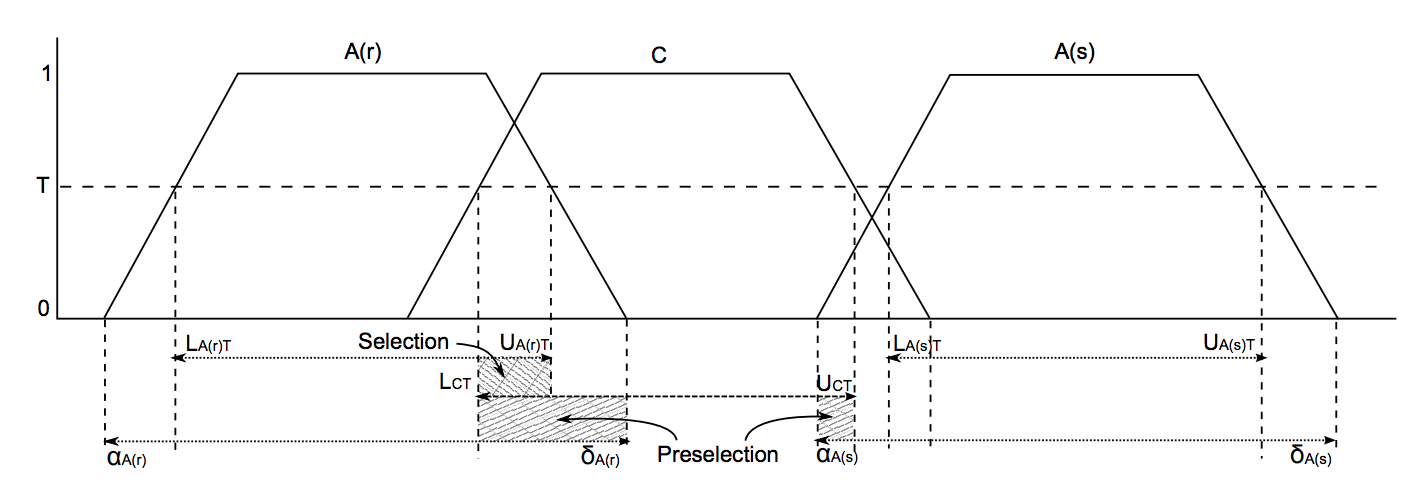
\includegraphics[width=0.9\textwidth]{gfx/preselection.png}
  \caption{\label{fig:preselection}Ejemplo de preselección y selección.}
\end{figure}

\subsection{Implementación de operadores difusos}

Para poder trabajar con cláusulas difusas, se han realizado extensiones de los operados descritos en \ref{mongooperators} para las medidas de posibilidad y necesidad.

Los operadores difusos son operadores ternarios que reciben los siguientes parámetros:

\begin{itemize}
    \item \textbf{field\_name}: Nombre del campo a evaluar. El campo tiene que corresponder con un atributo difuso cuyo valor debe ser un array de cuatro posiciones. 
    \item \textbf{value}: Trapezoide de referencia que estamos comparando.
    \item \textbf{threshold}: Grado mínimo pertenencia que debe cumplir el trapezoide a evaluar para superar el mínimo pedido.
\end{itemize}

Para la etapa de preselección debemos de calcular los cortes inferior y superior, L\_CT y U\_CT, respectivamente con respecto al trapezoide de referencia (el que se pretende comparar con los de la base de datos) y dar ciertas condiciones que deben de verificar alguno de los valores del array de la base de datos con respecto a estos cortes. La etapa de selección consiste en comparar los cortes calculados previamente con los cortes calculados sobre cada uno de los trapezoides almacenados en la base de datos. 

Sean $A$ y $B$ dos distribuciones de posibilidad trapezoidales definidas sobre un dominio ordenado $\Omega$, con $A = \trapezoidA$ y $B=\trapezoidB$ y $T \in [0,1]$ el parámetro \textit{threshold}. Vamos a definir los distintos operadores difusos dependiende del tipo de medida para posibilidad y necesidad.

\subsection{Operador THOLD}

El operador \texttt{\$thold} es un operador que aceptaremos como parámetro extra para todos los operadores difusos, será opcional y en caso de especificarse deberá contener un número entre $0$ y $1$. Será el grado de pertenencia mínimo que esperamos para el valor especificado. Si no se especifica, se tomará por defecto el valor $0$.

\subsection{Operador FEQ}

El operador \texttt{\$feq(A,T)} filtra los documentos $B$ que son \textit{posiblemente} iguales que $A$ para el umbral $T$.

Se calculan los cortes inferior y superior para el trapezoide $A$ \cite{indexingstrategies}:
%
\begin{align*}
    L_{CT} &= T * \beta_A + (1-T)\alpha_A \\
    U_{CT} &= T * \gamma_A + (1-T)\delta_A \\
\end{align*}
%
La etapa de preselección se calcula evaluando:
%
\begin{align*}
    \alpha_B &\leq U_{CT} \\
    \delta_B &\geq L_{CT} \\
\end{align*}
%
Y los elementos seleccionados finalmente son los que cumplan:
%
\begin{align*}
    L_B &\leq U_{CT} \\
    U_B &\geq L_{CT} \\
\end{align*}
%
donde $L_B$ y $U_B$ son los cortes inferior y superior respectivamente para cada documento de la base de datos calculados con las mismas ecuaciones que han calculado $U_{CT}$ y $L_{CT}$ pero con los valores de $B$.
La implementación de este operador puede verse en el apéndice \ref{appendix:code} entre las líneas \ref{code:feq:start} y \ref{code:feq:end}.

\begin{example}
Veamos un ejemplo de una consulta utilizando el operador \texttt{\$feq}:
%
\begin{verbatim}
{"superficie": {"$feq": [80,90,110,120]}}
\end{verbatim}
%
Especificando un umbral mínimo de 0.6:
%
\begin{verbatim}         
{"superficie": {"$feq": [80,90,110,120], "$thold": 0.6}}
\end{verbatim}

\end{example}

\subsection{Operador NFEQ}

El operador \texttt{\$nfeq(A,T)} filtra los documentos $B$ que son \textit{necesariamente} iguales que $A$ para el umbral $T$.

Se calculan los cortes inferior y superior para el trapezoide $A$ \cite{indexingneccesary}:
%
\begin{align*}
    L_{CT} &= T * \beta_A + (1-T)\alpha_A \\
    U_{CT} &= T * \gamma_A + (1-T)\delta_A \\
\end{align*}
%
La etapa de preselección se calcula evaluando:
%
\begin{align*}
    \beta_B &\geq L_{CT} \\
    \gamma_B &\leq U_{CT} \\
\end{align*}
%
Y los elementos seleccionados finalmente son los que cumplan:
%
\begin{align*}
    U_B &\leq U_{CT} \\
    L_B &\geq L_{CT} \\
\end{align*}
%
donde $L_B$ y $U_B$ son los cortes inferior y superior respectivamente para cada documento de la base de datos dado por:
%
\begin{align*}
    L_B &= T * \alpha_B + (1-T)\beta_B \\
    U_B &= T * \delta_B + (1-T)\gamma_B \\
\end{align*}
%
La implementación de este operador puede verse en el apéndice \ref{appendix:code} entre las líneas \ref{code:nfeq:start} y \ref{code:nfeq:end}.

\begin{example}
Veamos un ejemplo de una consulta utilizando el operador \texttt{\$nfeq}:
%
\begin{verbatim}
{"superficie": {"$nfeq": [80,90,110,120]}}
\end{verbatim}
%
Especificando un umbral mínimo de 0.4:
%
\begin{verbatim}         
{"superficie": {"$nfeq": [80,90,110,120], "$thold": 0.4}}
\end{verbatim}

\end{example}

\subsection{Operador FGT}

El operador \texttt{\$fgt(A,T)} filtra los documentos $B$ que son \textit{posiblemente} mayores que $A$ para el umbral $T$.

En este caso, no hay corte superior, por lo que solo calculamos el inferior:
%
\begin{align*}
    L_{CT} &= T * \delta_A + (1-T)\gamma_A \\
\end{align*}
%
La etapa de preselección se calcula evaluando:
%
\begin{align*}
    \delta_B \geq L_{CT}
\end{align*}
%
Y los elementos seleccionados finalmente son los que cumplan:
%
\begin{align*}
    L_B \geq L_{CT} \\
\end{align*}
%
donde $L_B$ es el corte inferior para cada documento de la base de datos dado por:
%
\begin{align*}
    L_B &= T * \gamma_B + (1-T)\delta_B
\end{align*}
%
La implementación de este operador puede verse en el apéndice \ref{appendix:code} entre las líneas \ref{code:fgt:start} y \ref{code:fgt:end}.

\begin{example}
Veamos un ejemplo de una consulta utilizando el operador \texttt{\$fgt}:
%
\begin{verbatim}
{"superficie": {"$fgt": [80,90,110,120]}}
\end{verbatim}

\end{example}

\subsection{Operador NFGT}

El operador \texttt{\$nfgt(A,T)} filtra los documentos $B$ que son \textit{necesariamente} mayores que $A$ para el umbral $T$.

En este caso, no hay corte superior, por lo que solo calculamos el inferior:
%
\begin{align*}
    L_{CT} &= T * \delta_A + (1-T)\gamma_A \\
\end{align*}
%
La etapa de preselección se calcula evaluando:
%
\begin{align*}
    \beta_B \geq L_{CT}
\end{align*}
%
Y los elementos seleccionados finalmente son los que cumplan:
%
\begin{align*}
    L_B \geq L_{CT} \\
\end{align*}
%
donde $L_B$ es el corte inferior para cada documento de la base de datos dado por:
%
\begin{align*}
    L_B &= T * \alpha_B + (1-T)\beta_B
\end{align*}
%
La implementación de este operador puede verse en el apéndice \ref{appendix:code} entre las líneas \ref{code:nfgt:start} y \ref{code:nfgt:end}.

\begin{example}
Veamos un ejemplo de una consulta utilizando el operador \texttt{\$nfgt}:
%
\begin{verbatim}
{"superficie": {"$nfgt": [80,90,110,120]}}
\end{verbatim}

\end{example}

\subsection{Operador FGTE}

El operador \texttt{\$fgte(A,T)} filtra los documentos $B$ que son \textit{posiblemente} mayores o iguales que $A$ para el umbral $T$.

En este caso, no hay corte superior, por lo que solo calculamos el inferior:
%
\begin{align*}
    L_{CT} &= T * \beta_A + (1-T)\alpha_A \\
\end{align*}
%
La etapa de preselección se calcula evaluando:
%
\begin{align*}
    \delta_B \geq L_{CT}
\end{align*}
%
Y los elementos seleccionados finalmente son los que cumplan:
%
\begin{align*}
    L_B \geq L_{CT} \\
\end{align*}
%
donde $L_B$ es el corte inferior para cada documento de la base de datos dado por:
%
\begin{align*}
    L_B &= T * \gamma_B + (1-T)\delta_B
\end{align*}
%
La implementación de este operador puede verse en el apéndice \ref{appendix:code} entre las líneas \ref{code:fgte:start} y \ref{code:fgte:end}.

\begin{example}
Veamos un ejemplo de una consulta utilizando el operador \texttt{\$fgte}:
%
\begin{verbatim}
{"superficie": {"$fgte": [80,90,110,120]}}
\end{verbatim}

\end{example}

\subsection{Operador NFGTE}

El operador \texttt{\$nfgte(A,T)} filtra los documentos $B$ que son \textit{necesariamente} mayores o iguales que $A$ para el umbral $T$.

En este caso, no hay corte superior, por lo que solo calculamos el inferior:
%
\begin{align*}
    L_{CT} &= T * \beta_A + (1-T)\alpha_A \\
\end{align*}
%
La etapa de preselección se calcula evaluando:
%
\begin{align*}
    \beta_B \geq L_{CT}
\end{align*}
%
Y los elementos seleccionados finalmente son los que cumplan:
%
\begin{align*}
    L_B \geq L_{CT} \\
\end{align*}
%
donde $L_B$ es el corte inferior para cada documento de la base de datos dado por:
%
\begin{align*}
    L_B &= T * \alpha_B + (1-T)\beta_B
\end{align*}
%
La implementación de este operador puede verse en el apéndice \ref{appendix:code} entre las líneas \ref{code:nfgte:start} y \ref{code:nfgte:end}.

\begin{example}
Veamos un ejemplo de una consulta utilizando el operador \texttt{\$nfgte}:
%
\begin{verbatim}
{"superficie": {"$nfgte": [80,90,110,120]}}
\end{verbatim}

\end{example}

\subsection{Operador FLT}

El operador \texttt{\$flt(A,T)} filtra los documentos $B$ que son \textit{posiblemente} menores que $A$ para el umbral $T$.

En este caso, no hay corte inferior, por lo que solo calculamos el superior:
%
\begin{align*}
    U_{CT} &= T * \alpha_A + (1-T)\beta_A \\
\end{align*}
%
La etapa de preselección se calcula evaluando:
%
\begin{align*}
    \alpha_B \leq U_{CT}
\end{align*}
%
Y los elementos seleccionados finalmente son los que cumplan:
%
\begin{align*}
    U_B \leq U_{CT} \\
\end{align*}
%
donde $U_B$ es el corte inferior para cada documento de la base de datos dado por:
%
\begin{align*}
    U_B &= T * \beta_B + (1-T)\alpha_B
\end{align*}
%
La implementación de este operador puede verse en el apéndice \ref{appendix:code} entre las líneas \ref{code:flt:start} y \ref{code:flt:end}.

\begin{example}
Veamos un ejemplo de una consulta utilizando el operador \texttt{\$flt}:
%
\begin{verbatim}
{"superficie": {"$flt": [80,90,110,120]}}
\end{verbatim}

\end{example}

\subsection{Operador NFLT}

El operador \texttt{\$nflt(A,T)} filtra los documentos $B$ que son \textit{necesariamente} menores que $A$ para el umbral $T$.

En este caso, no hay corte inferior, por lo que solo calculamos el superior:
%
\begin{align*}
    U_{CT} &= T * \alpha_A + (1-T)\beta_A \\
\end{align*}
%
La etapa de preselección se calcula evaluando:
%
\begin{align*}
    \gamma_B \leq U_{CT}
\end{align*}
%
Y los elementos seleccionados finalmente son los que cumplan:
%
\begin{align*}
    U_B \leq U_{CT} \\
\end{align*}
%
donde $U_B$ es el corte inferior para cada documento de la base de datos dado por:
%
\begin{align*}
    U_B &= T * \delta_B + (1-T)\gamma_B
\end{align*}
%
La implementación de este operador puede verse en el apéndice \ref{appendix:code} entre las líneas \ref{code:nflt:start} y \ref{code:nflt:end}.

\begin{example}
Veamos un ejemplo de una consulta utilizando el operador \texttt{\$nflt}:
%
\begin{verbatim}
{"superficie": {"$nflt": [80,90,110,120]}}
\end{verbatim}

\end{example}

\subsection{Operador FLTE}

El operador \texttt{\$flte(A,T)} filtra los documentos $B$ que son \textit{posiblemente} menores o iguales que $A$ para el umbral $T$.

En este caso, no hay corte inferior, por lo que solo calculamos el superior:
%
\begin{align*}
    U_{CT} &= T * \gamma_A + (1-T)\delta_A \\
\end{align*}
%
La etapa de preselección se calcula evaluando:
%
\begin{align*}
    \alpha_B \leq U_{CT}
\end{align*}
%
Y los elementos seleccionados finalmente son los que cumplan:
%
\begin{align*}
    U_B \leq U_{CT} \\
\end{align*}
%
donde $U_B$ es el corte inferior para cada documento de la base de datos dado por:
%
\begin{align*}
    U_B &= T * \beta_B + (1-T)\alpha_B
\end{align*}
%
La implementación de este operador puede verse en el apéndice \ref{appendix:code} entre las líneas \ref{code:flte:start} y \ref{code:flte:end}.

\begin{example}
Veamos un ejemplo de una consulta utilizando el operador \texttt{\$flte}:
%
\begin{verbatim}
{"superficie": {"$flte": [80,90,110,120]}}
\end{verbatim}

\end{example}

\subsection{Operador NFLTE}

El operador \texttt{\$nflte(A,T)} filtra los documentos $B$ que son \textit{necesariamente} menores o iguales que $A$ para el umbral $T$.

En este caso, no hay corte inferior, por lo que solo calculamos el superior:
%
\begin{align*}
    U_{CT} &= T * \gamma_A + (1-T)\delta_A \\
\end{align*}
%
La etapa de preselección se calcula evaluando:
%
\begin{align*}
    \gamma_B \leq U_{CT}
\end{align*}
%
Y los elementos seleccionados finalmente son los que cumplan:
%
\begin{align*}
    U_B \leq U_{CT} \\
\end{align*}
%
donde $U_B$ es el corte inferior para cada documento de la base de datos dado por:
%
\begin{align*}
    U_B &= T * \delta_B + (1-T)\gamma_B
\end{align*}
%
La implementación de este operador puede verse en el apéndice \ref{appendix:code} entre las líneas \ref{code:nflte:start} y \ref{code:nflte:end}.

\begin{example}
Veamos un ejemplo de una consulta utilizando el operador \texttt{\$nflte}:
%
\begin{verbatim}
{"superficie": {"$nflte": [80,90,110,120]}}
\end{verbatim}

\end{example}


\chapter{Conclusiones y vías futuras}
\section{Conclusiones y vías futuras}

En conclusión, hemos visto como se puede extender la funcionalidad de MongoDB para trabajar con conjuntos difusos. Se ha dado una solución con la implementación de la función \texttt{fuzzy\_find} que permite realizar consultas con cláusulas difusas y proyectar el grado de pertenencia a la consulta pedida, pero aún con ciertas limitaciones.

Esta versión de \texttt{fuzzy\_find} solo acepta una cláusula difusa por atributo, además no se pueden combinar cláusulas difusas para el mismo atributo.

Las vías futuras para extender esta funcionalidad pueden resumirse:

\begin{itemize}
    \item Mejorar restricciones: Hay que ampliar la funcionalidad de la función \texttt{fuzzy\_find} para permitir varias cláusulas difusas para un mismo atributo. Además, si se consigue esto, hay que modificar la proyección para poder seleccionar cuales de las condiciones difusas se quiere proyectar.
    \item Implementación de operadores lógicos: Hay que implementar los operadores lógicos para utilizar con cláusulas difusas.
    \item Mejorar indexación: MongoDB permite la indexación en campos de tipo array, un posible estudio de la indexación podría mejorar los tiempos de consulta.
    \item Extender funcionalidad en clientes MongoDB: Ahora mismo, la función \texttt{fuzzy\_find} está probada desde la shell de MongoDB. Un posible trabajo futuro sería extender esta funcionalidad a las librerías para los distintos lenguajes de programación.
    \item Aumentar funcionalidad MongoDB: En esta propuesta nos hemos centrado en el operador de agregación \textit{pipeline}. Se podría estudiar para implementar el trabajo con información imprecisa con el resto de operadores.
\end{itemize}

% ********************************************************************
% Backmatter
%*******************************************************
%\renewcommand{\thechapter}{\alph{chapter}}
\appendix
\part*{Anexo}
\chapter{Implementación Fuzzy Find}
\label{appendix:code}
\begin{lstlisting}[language=java, escapechar=|]
/////////////////////////
//                     //
//  MATCHES functions  //
//                     //
/////////////////////////

function feq(field_name, value, threshold) { |\label{code:feq:start}|
  let field_0 = field_name + '.0';
  let field_3 = field_name + '.3';
  let one_thold = 1 - threshold;
  let L_CT = threshold * value[1] + one_thold * value[0];
  let U_CT = threshold * value[2] + one_thold * value[3];

  return {
    [field_0]: {$lte: U_CT},
    [field_3]: {$gte: L_CT},
    $expr: {
      $and: [
        {
          $lte: [
            {
              $add: [
                {$multiply: [{$arrayElemAt: ['$' + field_name, 1]}, threshold]},
                {$multiply: [{$arrayElemAt: ['$' + field_name, 0]}, one_thold]}
              ]
            },
            U_CT
          ]
        },
        {
          $gte: [
            {
              $add: [
                {$multiply: [{$arrayElemAt: ['$' + field_name, 2]}, threshold]},
                {$multiply: [{$arrayElemAt: ['$' + field_name, 3]}, one_thold]}
              ]
            },
            L_CT
          ]
        }
      ]
    }
  };
} |\label{code:feq:end}|

function fgt(field_name, value, threshold) { |\label{code:fgt:start}|
  let field_3 = field_name + '.3';
  let one_thold = 1 - threshold;
  let L_CT = threshold * value[3] + one_thold * value[2];

  return {
    [field_3]: {$gte: L_CT},
    $expr: {
      $gte: [
        {
          $add: [
            {$multiply: [{$arrayElemAt: ['$' + field_name, 2]}, threshold]},
            {$multiply: [{$arrayElemAt: ['$' + field_name, 3]}, one_thold]}
          ]
        },
        L_CT
      ]
    }
  }
} |\label{code:fgt:end}|

function fgte(field_name, value, threshold) { |\label{code:fgte:start}|
  let field_3 = field_name + '.3';
  let one_thold = 1 - threshold;
  let L_CT = threshold * value[1] + one_thold * value[0];

  return {
    [field_3]: {$gte: L_CT},
    $expr: {
      $gte: [
        {
          $add: [
            {$multiply: [{$arrayElemAt: ['$' + field_name, 2]}, threshold]},
            {$multiply: [{$arrayElemAt: ['$' + field_name, 3]}, one_thold]}
          ]
        },
        L_CT
      ]
    }
  }
} |\label{code:fgte:end}|

function flt(field_name, value, threshold) { |\label{code:flt:start}|
  let field_0 = field_name + '.0';
  let one_thold = 1 - threshold;
  let U_CT = threshold * value[0] + one_thold * value[1];

  return {
    [field_0]: {$lte: U_CT},
    $expr: {
      $lte: [
        {
          $add: [
            {$multiply: [{$arrayElemAt: ['$' + field_name, 1]}, threshold]},
            {$multiply: [{$arrayElemAt: ['$' + field_name, 0]}, one_thold]}
          ]
        },
        U_CT
      ]
    }
  }
} |\label{code:flt:end}|

function flte(field_name, value, threshold) { |\label{code:flte:start}|
  let field_0 = field_name + '.0';
  let one_thold = 1 - threshold;
  let U_CT = threshold * value[2] + one_thold * value[3];

  return {
    [field_0]: {$lte: U_CT},
    $expr: {
      $lte: [
        {
          $add: [
            {$multiply: [{$arrayElemAt: ['$' + field_name, 1]}, threshold]},
            {$multiply: [{$arrayElemAt: ['$' + field_name, 0]}, one_thold]}
          ]
        },
        U_CT
      ]
    }
  }
} |\label{code:flte:end}|

function nfeq(field_name, value, threshold) { |\label{code:nfeq:start}|
  let field_1 = field_name + '.1';
  let field_2 = field_name + '.2';
  let one_thold = 1 - threshold;
  let L_CT = threshold * value[1] + one_thold * value[0];
  let U_CT = threshold * value[2] + one_thold * value[3];

  return {
    [field_1]: {$gte: L_CT},
    [field_2]: {$lte: U_CT},
    $expr: {
      $and: [
        {
          $lte: [
            {
              $add: [
                {$multiply: [{$arrayElemAt: ['$' + field_name, 3]}, threshold]},
                {$multiply: [{$arrayElemAt: ['$' + field_name, 2]}, one_thold]}
              ]
            },
            U_CT
          ]
        },
        {
          $gte: [
            {
              $add: [
                {$multiply: [{$arrayElemAt: ['$' + field_name, 0]}, threshold]},
                {$multiply: [{$arrayElemAt: ['$' + field_name, 1]}, one_thold]}
              ]
            },
            L_CT
          ]
        }
      ]
    }
  };
} |\label{code:nfeq:end}|

function nfgt(field_name, value, threshold) { |\label{code:nfgt:start}|
  let field_1 = field_name + '.1';
  let one_thold = 1 - threshold;
  let L_CT = threshold * value[3] + one_thold * value[2];

  return {
    [field_1]: {$gte: L_CT},
    $expr: {
      $gte: [
        {
          $add: [
            {$multiply: [{$arrayElemAt: ['$' + field_name, 0]}, threshold]},
            {$multiply: [{$arrayElemAt: ['$' + field_name, 1]}, one_thold]}
          ]
        },
        L_CT
      ]
    }
  }
} |\label{code:nfgt:end}|

function nfgte(field_name, value, threshold) { |\label{code:nfgte:start}|
  let field_1 = field_name + '.1';
  let one_thold = 1 - threshold;
  let L_CT = threshold * value[1] + one_thold * value[0];

  return {
    [field_1]: {$gte: L_CT},
    $expr: {
      $gte: [
        {
          $add: [
            {$multiply: [{$arrayElemAt: ['$' + field_name, 0]}, threshold]},
            {$multiply: [{$arrayElemAt: ['$' + field_name, 1]}, one_thold]}
          ]
        },
        L_CT
      ]
    }
  }
} |\label{code:nfgte:end}|

function nflt(field_name, value, threshold) { |\label{code:nflt:start}|
  let field_2 = field_name + '.2';
  let one_thold = 1 - threshold;
  let U_CT = threshold * value[0] + one_thold * value[1];

  return {
    [field_2]: {$lte: U_CT},
    $expr: {
      $lte: [
        {
          $add: [
            {$multiply: [{$arrayElemAt: ['$' + field_name, 3]}, threshold]},
            {$multiply: [{$arrayElemAt: ['$' + field_name, 2]}, one_thold]}
          ]
        },
        U_CT
      ]
    }
  }
} |\label{code:nflt:end}|

function nflte(field_name, value, threshold) { |\label{code:nflte:start}|
  let field_2 = field_name + '.2';
  let one_thold = 1 - threshold;
  let U_CT = threshold * value[2] + one_thold * value[3];

  return {
    [field_2]: {$lte: U_CT},
    $expr: {
      $lte: [
        {
          $add: [
            {$multiply: [{$arrayElemAt: ['$' + field_name, 3]}, threshold]},
            {$multiply: [{$arrayElemAt: ['$' + field_name, 2]}, one_thold]}
          ]
        },
        U_CT
      ]
    }
  }
} |\label{code:nflte:end}|

/////////////////////////////
//                         //
//  end MATCHES functions  //
//                         //
/////////////////////////////

/////////////////////////////
//                         //
//  PROJECTION functions   //
//                         //
/////////////////////////////

function feq_cdeg(field_name, value) {
  return {
    $cond: [
      {
        $and: [
          {$gte: [{$arrayElemAt: ['$' + field_name, 2]}, value[1]]},
          {$lte: [{$arrayElemAt: ['$' + field_name, 1]}, value[2]]}
        ]
      },
      1,
      {
        $cond: [
          {
            $or: [
              {$lte: [{$arrayElemAt: ['$' + field_name, 3]}, value[0]]},
              {$gte: [{$arrayElemAt: ['$' + field_name, 0]}, value[3]]}
            ]
          },
          0,
          {
            $cond: [
              {
                $and: [
                  {$gt: [{$arrayElemAt: ['$' + field_name, 3]}, value[0]]},
                  {$lt: [{$arrayElemAt: ['$' + field_name, 2]}, value[1]]}
                ]
              },
              {
                $divide: [
                  {
                    $subtract: [
                      {$arrayElemAt: ['$' + field_name, 3]},
                      value[0]
                    ]
                  },
                  {
                    $subtract: [
                      {
                        $subtract: [
                          value[1],
                          value[0]
                        ]
                      },
                      {
                        $subtract: [
                          {$arrayElemAt: ['$' + field_name, 2]},
                          {$arrayElemAt: ['$' + field_name, 3]}
                        ]
                      }
                    ]
                  }
                ]
              },
              {
                $divide: [
                  {
                    $subtract: [
                      value[3],
                      {$arrayElemAt: ['$' + field_name, 0]}
                    ]
                  },
                  {
                    $subtract: [
                      {
                        $subtract: [
                          {$arrayElemAt: ['$' + field_name, 1]},
                          {$arrayElemAt: ['$' + field_name, 0]}
                        ]
                      },
                      {
                        $subtract: [
                          value[2],
                          value[3]
                        ]
                      }
                    ]
                  }
                ]
              }
            ]
          }
        ]
      }
    ]
  };
}

function fgt_cdeg(field_name, value) {
  return {
    $cond: [
      {$gte: [{$arrayElemAt: ['$' + field_name, 2]}, value[3]]},
      1,
      {
        $cond: [
          {$lte: [{$arrayElemAt: ['$' + field_name, 3]}, value[2]]},
          0,
          {
            $divide: [
              {
                $subtract: [
                  {$arrayElemAt: ['$' + field_name, 3]},
                  value[2]
                ]
              },
              {
                $subtract: [
                  {
                    $subtract: [
                      value[3],
                      value[2]
                    ]
                  },
                  {
                    $subtract: [
                      {$arrayElemAt: ['$' + field_name, 2]},
                      {$arrayElemAt: ['$' + field_name, 3]}
                    ]
                  }
                ]
              }
            ]
          }
        ]
      }
    ]
  };
}

function flt_cdeg(field_name, value) {
  return {
    $cond: [
      {$lte: [{$arrayElemAt: ['$' + field_name, 1]}, value[0]]},
      1,
      {
        $cond: [
          {$gte: [{$arrayElemAt: ['$' + field_name, 0]}, value[1]]},
          0,
          {
            $divide: [
              {
                $subtract: [
                  {$arrayElemAt: ['$' + field_name, 0]},
                  value[1]
                ]
              },
              {
                $subtract: [
                  {
                    $subtract: [
                      value[0],
                      value[1]
                    ]
                  },
                  {
                    $subtract: [
                      {$arrayElemAt: ['$' + field_name, 1]},
                      {$arrayElemAt: ['$' + field_name, 0]}
                    ]
                  }
                ]
              }
            ]
          }
        ]
      }
    ]
  };
}

function fgte_cdeg(field_name, value) {
  return {
    $cond: [
      {$gte: [{$arrayElemAt: ['$' + field_name, 2]}, value[1]]},
      1,
      {
        $cond: [
          {$lte: [{$arrayElemAt: ['$' + field_name, 3]}, value[0]]},
          0,
          {
            $divide: [
              {
                $subtract: [
                  {$arrayElemAt: ['$' + field_name, 3]},
                  value[0]
                ]
              },
              {
                $subtract: [
                  {
                    $subtract: [
                      value[1],
                      value[0]
                    ]
                  },
                  {
                    $subtract: [
                      {$arrayElemAt: ['$' + field_name, 2]},
                      {$arrayElemAt: ['$' + field_name, 3]}
                    ]
                  }
                ]
              }
            ]
          }
        ]
      }
    ]
  };
}

function flte_cdeg(field_name, value) {
  return {
    $cond: [
      {$lte: [{$arrayElemAt: ['$' + field_name, 1]}, value[2]]},
      1,
      {
        $cond: [
          {$gte: [{$arrayElemAt: ['$' + field_name, 0]}, value[3]]},
          0,
          {
            $divide: [
              {
                $subtract: [
                  value[3],
                  {$arrayElemAt: ['$' + field_name, 0]}
                ]
              },
              {
                $subtract: [
                  {
                    $subtract: [
                      {$arrayElemAt: ['$' + field_name, 1]},
                      {$arrayElemAt: ['$' + field_name, 0]}
                    ]
                  },
                  {
                    $subtract: [
                      value[2],
                      value[3]
                    ]
                  }
                ]
              }
            ]
          }
        ]
      }
    ]
  };
}

function nfeq_cdeg(field_name, value) {
  return {
    $cond: [
      {
        $or: [
          {
            $and: [
              {$lte: [{$arrayElemAt: ['$' + field_name, 1]}, value[0]]},
              {$eq: [{$arrayElemAt: ['$' + field_name, 0]}, value[1]]}
            ]
          },
          {
            $and: [
              {$gte: [{$arrayElemAt: ['$' + field_name, 2]}, value[3]]},
              {$eq: [{$arrayElemAt: ['$' + field_name, 3]}, value[2]]}
            ]
          }
        ]
      },
      0,
      {
        $cond: [
          {$lt: [{$arrayElemAt: ['$' + field_name, 0]}, value[1]]},
          {
            $cond: [
              {$gt: [{$arrayElemAt: ['$' + field_name, 3]}, value[2]]},
              {
                $min: [
                  {
                    $divide: [
                      {
                        $subtract: [
                          {$arrayElemAt: ['$' + field_name, 1]},
                          value[0]
                        ]
                      },
                      {
                        $subtract: [
                          {
                            $subtract: [
                              value[1],
                              value[0]
                            ]
                          },
                          {
                            $subtract: [
                              {$arrayElemAt: ['$' + field_name, 0]},
                              {$arrayElemAt: ['$' + field_name, 1]}
                            ]
                          }
                        ]
                      }
                    ]
                  },
                  {
                    $divide: [
                      {
                        $subtract: [
                          {$arrayElemAt: ['$' + field_name, 2]},
                          value[3]
                        ]
                      },
                      {
                        $subtract: [
                          {
                            $subtract: [
                              value[2],
                              value[3]
                            ]
                          },
                          {
                            $subtract: [
                              {$arrayElemAt: ['$' + field_name, 3]},
                              {$arrayElemAt: ['$' + field_name, 2]}
                            ]
                          }
                        ]
                      }
                    ]
                  }
                ]
              },
              {
                $divide: [
                  {
                    $subtract: [
                      {$arrayElemAt: ['$' + field_name, 1]},
                      value[0]
                    ]
                  },
                  {
                    $subtract: [
                      {
                        $subtract: [
                          value[1],
                          value[0]
                        ]
                      },
                      {
                        $subtract: [
                          {$arrayElemAt: ['$' + field_name, 0]},
                          {$arrayElemAt: ['$' + field_name, 1]}
                        ]
                      }
                    ]
                  }
                ]
              }
            ]
          },
          {
            $cond: [
              {$gt: [{$arrayElemAt: ['$' + field_name, 3]}, value[2]]},
              {
                $divide: [
                  {
                    $subtract: [
                      {$arrayElemAt: ['$' + field_name, 2]},
                      value[3]
                    ]
                  },
                  {
                    $subtract: [
                      {
                        $subtract: [
                          value[2],
                          value[3]
                        ]
                      },
                      {
                        $subtract: [
                          {$arrayElemAt: ['$' + field_name, 3]},
                          {$arrayElemAt: ['$' + field_name, 2]}
                        ]
                      }
                    ]
                  }
                ]
              },
              1
            ]
          }
        ]
      }
    ]
  };
}

function nfgt_cdeg(field_name, value) {
  return {
    $cond: [
      {$gte: [{$arrayElemAt: ['$' + field_name, 0]}, value[3]]},
      1,
      {
        $cond: [
          {$lte: [{$arrayElemAt: ['$' + field_name, 1]}, value[2]]},
          0,
          {
            $divide: [
              {
                $subtract: [
                  {$arrayElemAt: ['$' + field_name, 1]},
                  value[2]
                ]
              },
              {
                $subtract: [
                  {
                    $subtract: [
                      value[3],
                      value[2]
                    ]
                  },
                  {
                    $subtract: [
                      {$arrayElemAt: ['$' + field_name, 0]},
                      {$arrayElemAt: ['$' + field_name, 1]}
                    ]
                  }
                ]
              }
            ]
          }
        ]
      }
    ]
  };
}

function nfgte_cdeg(field_name, value) {
  return {
    $cond: [
      {$gte: [{$arrayElemAt: ['$' + field_name, 0]}, value[1]]},
      1,
      {
        $cond: [
          {$lte: [{$arrayElemAt: ['$' + field_name, 1]}, value[0]]},
          0,
          {
            $divide: [
              {
                $subtract: [
                  {$arrayElemAt: ['$' + field_name, 1]},
                  value[0]
                ]
              },
              {
                $subtract: [
                  {
                    $subtract: [
                      value[1],
                      value[0]
                    ]
                  },
                  {
                    $subtract: [
                      {$arrayElemAt: ['$' + field_name, 0]},
                      {$arrayElemAt: ['$' + field_name, 1]}
                    ]
                  }
                ]
              }
            ]
          }
        ]
      }
    ]
  };
}

function nflt_cdeg(field_name, value) {
  return {
    $cond: [
      {$lte: [{$arrayElemAt: ['$' + field_name, 3]}, value[0]]},
      1,
      {
        $cond: [
          {$gte: [{$arrayElemAt: ['$' + field_name, 2]}, value[1]]},
          0,
          {
            $divide: [
              {
                $subtract: [
                  {$arrayElemAt: ['$' + field_name, 2]},
                  value[1]
                ]
              },
              {
                $subtract: [
                  {
                    $subtract: [
                      value[0],
                      value[1]
                    ]
                  },
                  {
                    $subtract: [
                      {$arrayElemAt: ['$' + field_name, 3]},
                      {$arrayElemAt: ['$' + field_name, 2]}
                    ]
                  }
                ]
              }
            ]
          }
        ]
      }
    ]
  };
}

function nflte_cdeg(field_name, value) {
  return {
    $cond: [
      {$lte: [{$arrayElemAt: ['$' + field_name, 3]}, value[2]]},
      1,
      {
        $cond: [
          {$gte: [{$arrayElemAt: ['$' + field_name, 2]}, value[3]]},
          0,
          {
            $divide: [
              {
                $subtract: [
                  value[3],
                  {$arrayElemAt: ['$' + field_name, 2]}
                ]
              },
              {
                $subtract: [
                  {
                    $subtract: [
                      {$arrayElemAt: ['$' + field_name, 3]},
                      {$arrayElemAt: ['$' + field_name, 2]}
                    ]
                  },
                  {
                    $subtract: [
                      value[2],
                      value[3]
                    ]
                  }
                ]
              }
            ]
          }
        ]
      }
    ]
  };
}

////////////////////////////////
//                            //
//  end PROJECTION functions  //
//                            //
////////////////////////////////

function split_queries(query) {
  // remove all fuzzy properties
  let fuzzy_operators = ['$feq', '$fgt', '$fgte', '$flt', '$flte', '$nfeq', '$nfgt', '$nfgte', '$nflt', '$nflte'];
  let fquery = {};
  for (let property in query) {
    let prop_query = query[property];
    if (Object.prototype.toString.call(prop_query) === '[object Object]'
      || Object.prototype.toString.call(prop_query) === '[object BSON]') {
      let is_fuzzy = false;
      for (let i = 0; i < fuzzy_operators.length && !is_fuzzy; i++) {
        if (prop_query.hasOwnProperty(fuzzy_operators[i]))
          is_fuzzy = true;
      }

      if (is_fuzzy) {
        fquery[property] = prop_query;
        delete query[property]
      }
    }
  }

  return [query, fquery];
}

function trapezoid(x) {
  if (Object.prototype.toString.call(x) !== '[object Array]' &&
    Object.prototype.toString.call(x) !== '[object Number]')
    throw 'Incompatible type: ' + x + ' ' + Object.prototype.toString.call(x);

  if (Object.prototype.toString.call(x) === '[object Array]') {
    for (let i = 0; i < x.length; i++) {
      if (Object.prototype.toString.call(x[i]) !== '[object Number]')
        throw 'Incompatible type';
    }
  }

  let v = x;
  if (Object.prototype.toString.call(x) === '[object Number]')
    v = [x];

  v = v.sort();
  switch (v.length) {
    case 1:
      return [v[0], v[0], v[0], v[0]];
    case 2:
      return [v[0], v[0], v[1], v[1]];
    case 3:
      return [v[0], v[1], v[1], v[2]];
    case 4:
      return v;
    default:
      throw 'Length must be smaller than 4';
  }
}

function parse_fuzzy(fquery) {
  let fuzzy_operators = ['$feq', '$fgt', '$fgte', '$flt', '$flte', '$nfeq', '$nfgt', '$nfgte', '$nflt', '$nflte'];
  let query = {};
  let foperators = {};

  for (let fproperty in fquery) {
    let fsubquery = fquery[fproperty];

    for (let i = 0; i < fuzzy_operators.length; i++) {
      let operator = fuzzy_operators[i];

      if (fsubquery.hasOwnProperty(operator)) {

        if (foperators.hasOwnProperty(fproperty))
          foperators[fproperty].push(operator);
        else
          foperators[fproperty] = [operator];

        let func = operator.toString().substring(1);
        let value = trapezoid(fsubquery[operator]);
        let threshold = fsubquery.hasOwnProperty('$thold') ? fsubquery['$thold'] : 0;
        let to_eval = func + '("' + fproperty + '", [' + value + '], ' + threshold + ')';
        let match = eval(to_eval);
        for (let property in match) {
          query[property] = match[property];
        }
      }
    }
  }

  return [query, foperators];
}

function get_match(query, fquery) {
  let match_stage = {$match: {}};

  for (let property in query) {
    match_stage['$match'][property] = query[property];
  }
  for (let property in fquery) {
    match_stage['$match'][property] = fquery[property];
  }

  return match_stage;
}

function get_projection(fquery, foperators, projection) {
  let stage = {$project: {}};

  for (let property in projection) {
    if (property.includes('_cdeg') && projection[property] === 1) {
      let fproperty = property.replace('_cdeg', '');

      if (foperators[fproperty].length !== 1)
        throw 'Projection failed';

      let operator = foperators[fproperty][0];
      let func = operator.toString().substring(1);
      let value = trapezoid(fquery[fproperty][operator]);
      let to_eval = func + '_cdeg("' + fproperty + '", [' + value + '])';
      stage['$project'][property] = eval(to_eval);
    }
    else {
      stage['$project'][property] = projection[property];
    }
  }

  return stage;
}

function fuzzy_find(collection, filter, projection, count_name = null) {
  // 1. Check types
  if ((Object.prototype.toString.call(filter) !== '[object Object]' && Object.prototype.toString.call(filter) !== '[object BSON]') ||
    (Object.prototype.toString.call(projection) !== '[object Object]' && Object.prototype.toString.call(filter) !== '[object BSON]') ||
    (Object.prototype.toString.call(collection) !== '[object String]' && Object.prototype.toString.call(filter) !== '[object BSON]') ||
    (count_name !== null && Object.prototype.toString.call(count_name) !== '[object String]'))
    throw 'Incompatible type';

  let stages = [];
  let queries = split_queries(filter);
  let query = queries[0];
  let fuzzy = parse_fuzzy(queries[1]);
  let fquery = fuzzy[0];
  let foperators = fuzzy[1];

  stages.push(get_match(query, fquery));

  if (Object.keys(projection).length !== 0)  // check for empty object
    stages.push(get_projection(queries[1], foperators, projection));

  if (count_name !== null)
    stages.push({'$count': count_name});

  return db[collection].aggregate(stages);
}

// matches functions
db.system.js.save({_id: 'feq', value: feq});
db.system.js.save({_id: 'fgt', value: fgt});
db.system.js.save({_id: 'fgte', value: fgte});
db.system.js.save({_id: 'flt', value: flt});
db.system.js.save({_id: 'flte', value: flte});

db.system.js.save({_id: 'nfeq', value: nfeq});
db.system.js.save({_id: 'nfgt', value: nfgt});
db.system.js.save({_id: 'nfgte', value: nfgte});
db.system.js.save({_id: 'nflt', value: nflt});
db.system.js.save({_id: 'nflte', value: nflte});

// projection functions
db.system.js.save({_id: 'feq_cdeg', value: feq_cdeg});
db.system.js.save({_id: 'nfeq_cdeg', value: nfeq_cdeg});
db.system.js.save({_id: 'fgt_cdeg', value: fgt_cdeg});
db.system.js.save({_id: 'nfgt_cdeg', value: nfgt_cdeg});
db.system.js.save({_id: 'flt_cdeg', value: flt_cdeg});
db.system.js.save({_id: 'nflt_cdeg', value: nflt_cdeg});
db.system.js.save({_id: 'fgte_cdeg', value: fgte_cdeg});
db.system.js.save({_id: 'nfgte_cdeg', value: nfgte_cdeg});
db.system.js.save({_id: 'flte_cdeg', value: flte_cdeg});
db.system.js.save({_id: 'nflte_cdeg', value: nflte_cdeg});

// functions
db.system.js.save({_id: 'split_queries', value: split_queries});
db.system.js.save({_id: 'parse_fuzzy', value: parse_fuzzy});
db.system.js.save({_id: 'trapezoid', value: trapezoid});
db.system.js.save({_id: 'get_match', value: get_match});
db.system.js.save({_id: 'get_projection', value: get_projection});
db.system.js.save({_id: 'fuzzy_find', value: fuzzy_find});
\end{lstlisting}

%********************************************************************
% Other Stuff in the Back
%*******************************************************
\cleardoublepage%********************************************************************
% Bibliography
%*******************************************************
% work-around to have small caps also here in the headline
\manualmark
\markboth{\spacedlowsmallcaps{\bibname}}{\spacedlowsmallcaps{\bibname}} % work-around to have small caps also
%\phantomsection 
\refstepcounter{dummy}
\addtocontents{toc}{\protect\vspace{\beforebibskip}} % to have the bib a bit from the rest in the toc
\addcontentsline{toc}{chapter}{\tocEntry{\bibname}}
\label{app:bibliography}
\printbibliography

%\cleardoublepage%*******************************************************
% Declaration
%*******************************************************
\refstepcounter{dummy}
\pdfbookmark[0]{Declaration}{declaration}
\chapter*{Declaración}
\thispagestyle{empty}

% TODO - DNI
Yo, \myName, alumno de la titulación \emph{\myDegree} de la \emph{\myFaculty} y de la \emph{\myOtherFaculty} de la \emph{\myUni}, con DNI XXXXXXXXX, asumo la originalidad de este trabajo, entendida en el sentido de que no se han utilizado fuentes sin citarlas debídamente.

Y para que conste, expido y firmo la presente declaración.

\bigskip
 
\noindent\textit{\myLocation, } %TODO - DATE

\smallskip

\begin{flushright}
    \begin{tabular}{m{5cm}}
        \\ \hline
        \centering\myName \\
    \end{tabular}
\end{flushright}
%\cleardoublepage\pagestyle{empty}

\hfill

\vfill


\pdfbookmark[0]{Colophon}{colophon}
\section*{Colophon}
This document was typeset using the typographical look-and-feel \texttt{classicthesis} developed by Andr\'e Miede. 
The style was inspired by Robert Bringhurst's seminal book on typography ``\emph{The Elements of Typographic Style}''. 
\texttt{classicthesis} is available for both \LaTeX\ and \mLyX: 
\begin{center}
\url{https://bitbucket.org/amiede/classicthesis/}
\end{center}
Happy users of \texttt{classicthesis} usually send a real postcard to the author, a collection of postcards received so far is featured here: 
\begin{center}
\url{http://postcards.miede.de/}
\end{center}
 
\bigskip

\noindent\finalVersionString

%Hermann Zapf's \emph{Palatino} and \emph{Euler} type faces (Type~1 PostScript fonts \emph{URW
%Palladio L} and \emph{FPL}) are used. The ``typewriter'' text is typeset in \emph{Bera Mono}, 
%originally developed by Bitstream, Inc. as ``Bitstream Vera''. (Type~1 PostScript fonts were made 
%available by Malte Rosenau and
%Ulrich Dirr.)

%\paragraph{note:} The custom size of the textblock was calculated
%using the directions given by Mr. Bringhurst (pages 26--29 and
%175/176). 10~pt Palatino needs  133.21~pt for the string
%``abcdefghijklmnopqrstuvwxyz''. This yields a good line length between
%24--26~pc (288--312~pt). Using a ``\emph{double square textblock}''
%with a 1:2 ratio this results in a textblock of 312:624~pt (which
%includes the headline in this design). A good alternative would be the
%``\emph{golden section textblock}'' with a ratio of 1:1.62, here
%312:505.44~pt. For comparison, \texttt{DIV9} of the \texttt{typearea}
%package results in a line length of 389~pt (32.4~pc), which is by far
%too long. However, this information will only be of interest for
%hardcore pseudo-typographers like me.%
%
%To make your own calculations, use the following commands and look up
%the corresponding lengths in the book:
%\begin{verbatim}
%    \settowidth{\abcd}{abcdefghijklmnopqrstuvwxyz}
%    \the\abcd\ % prints the value of the length
%\end{verbatim}
%Please see the file \texttt{classicthesis.sty} for some precalculated 
%values for Palatino and Minion.
%
%    \settowidth{\abcd}{abcdefghijklmnopqrstuvwxyz}
%    \the\abcd\ % prints the value of the length
% ********************************************************************
% Game Over: Restore, Restart, or Quit?
%*******************************************************
\end{document}
% ********************************************************************